\documentclass[a4paper]{book}
\usepackage{a4wide}
\usepackage{makeidx}
\usepackage{graphicx}
\usepackage{multicol}
\usepackage{float}
\usepackage{listings}
\usepackage{color}
\usepackage{textcomp}
\usepackage{alltt}
\usepackage{times}
\usepackage{ifpdf}
\ifpdf
\usepackage[pdftex,
            pagebackref=true,
            colorlinks=true,
            linkcolor=blue,
            unicode
           ]{hyperref}
\else
\usepackage[ps2pdf,
            pagebackref=true,
            colorlinks=true,
            linkcolor=blue,
            unicode
           ]{hyperref}
\usepackage{pspicture}
\fi
\usepackage[utf8]{inputenc}
\usepackage{doxygen}
\lstset{language=C++,inputencoding=utf8,basicstyle=\footnotesize,breaklines=true,breakatwhitespace=true,tabsize=8,numbers=left }
\makeindex
\setcounter{tocdepth}{3}
\renewcommand{\footrulewidth}{0.4pt}
\begin{document}
\hypersetup{pageanchor=false}
\begin{titlepage}
\vspace*{7cm}
\begin{center}
{\Large PhysGameEngine \\[1ex]\large .01 }\\
\vspace*{1cm}
{\large Generated by Doxygen 1.6.3}\\
\vspace*{0.5cm}
{\small Sun May 9 13:59:14 2010}\\
\end{center}
\end{titlepage}
\clearemptydoublepage
\pagenumbering{roman}
\tableofcontents
\clearemptydoublepage
\pagenumbering{arabic}
\hypersetup{pageanchor=true}
\chapter{Physgame}
\label{index}\hypertarget{index}{}The Physgame engine is an abstraction layer between less portable, less user friendly, more sophistciated libraries and the game you want to make. If we do our jobs right this will save time and effort making and porting games between a variety of platforms. If you link only against this library, not a single line of your Standard compliant C++ code should need to change between platforms. At this early stage we are proving the concept with \char`\"{}Catch!\char`\"{} our first sample game. It Currently runs on Linux and Windows with an Identical codebase, when we are done with \char`\"{}Catch!\char`\"{} We want it to have one codebase, and downloadable in the Iphone app store, the Xbox store, on the PS3, on Steam, and in a variety of linux repositories.

To get the latest news on development checkout: \href{http://gitorious.org/physgame}{\tt http://gitorious.org/physgame} The wiki Which acts as our current Knowledge base: \href{http://gitorious.org/physgame/pages/Home}{\tt http://gitorious.org/physgame/pages/Home}\hypertarget{index_Engine}{}\section{Structure}\label{index_Engine}
\hyperlink{mainloop1}{Main Loop Flow}

Call Back Manager

Event Manager

Items in the world -\/ Actor Class \hypertarget{index_Data}{}\section{Types}\label{index_Data}
\hyperlink{classPhysVector3}{PhysVector3}

\hyperlink{classPhysEvent}{PhysEvent} 
\chapter{Main Loop Structure and Flow}
\label{mainloop1}
\hypertarget{mainloop1}{}
\begin{Desc}
\item[\hyperlink{todo__todo000032}{Todo}]create a lighting manager and put this in there \end{Desc}


The MainLoop is heart of most video games and simulations.\hypertarget{mainloop1_mainloopoverview1}{}\subsection{Main loop Overview}\label{mainloop1_mainloopoverview1}
The Main loop runs in \hyperlink{classMezzanine_1_1World_a7c19ed5889b3de00a6f475b5922f9545}{World.MainLoop()} which is called by default from \hyperlink{classMezzanine_1_1World_a72d6d82926bfbfca96c246f109f0fc58}{World::GameInit()}. By default this Method also starts the render, the physics andthe input systems. It does very little on it's own. The main loop then calls the PreMainLoopItems(), DoMainLoopItems and PreMainLoopItems(), for each manager in the order of their priority from Lowest to Highest. \par
 Here is a listing of default priorities for each of the managers the a world intantiates by default: -\/50 User Input and events -\/40 Actors -\/30 Physics -\/20 \hyperlink{classMezzanine_1_1Camera}{Camera} -\/10 Lighting (Not yet implemented) 0 Graphics 10 Sound 20 Resources 
\chapter{Todo List}
\label{todo}
\hypertarget{todo}{}
\label{todo__todo000003}
\hypertarget{todo__todo000003}{}
 
\begin{DoxyDescription}
\item[Page \hyperlink{MainLoop}{} ]actually document the gameloop 
\end{DoxyDescription}
\chapter{Namespace Index}
\section{Namespace List}
Here is a list of all namespaces with brief descriptions:\begin{DoxyCompactList}
\item\contentsline{section}{\hyperlink{namespaceOgre}{Ogre} }{\pageref{d1/ddd/namespaceOgre}}{}
\end{DoxyCompactList}

\chapter{Class Index}
\section{Class Hierarchy}
This inheritance list is sorted roughly, but not completely, alphabetically:\begin{DoxyCompactList}
\item \contentsline{section}{ActorBase}{\pageref{dd/d7b/classActorBase}}{}
\begin{DoxyCompactList}
\item \contentsline{section}{ActorDynRigid}{\pageref{d4/d0e/classActorDynRigid}}{}
\item \contentsline{section}{ActorDynSoft}{\pageref{dc/de0/classActorDynSoft}}{}
\item \contentsline{section}{ActorSta}{\pageref{d3/daf/classActorSta}}{}
\end{DoxyCompactList}
\item \contentsline{section}{MetaCode}{\pageref{d7/d72/classMetaCode}}{}
\item \contentsline{section}{PhysEvent}{\pageref{d9/dc2/classPhysEvent}}{}
\begin{DoxyCompactList}
\item \contentsline{section}{PhysEventRenderTime}{\pageref{d4/d83/classPhysEventRenderTime}}{}
\item \contentsline{section}{PhysEventUserInput}{\pageref{dc/d0e/classPhysEventUserInput}}{}
\end{DoxyCompactList}
\item \contentsline{section}{PhysEventManager}{\pageref{d5/dd7/classPhysEventManager}}{}
\item \contentsline{section}{PhysMotionState}{\pageref{d2/d14/classPhysMotionState}}{}
\item \contentsline{section}{PhysQuaternion}{\pageref{d5/d19/classPhysQuaternion}}{}
\item \contentsline{section}{PhysVector3}{\pageref{da/d11/classPhysVector3}}{}
\item \contentsline{section}{PhysWorld}{\pageref{db/df5/classPhysWorld}}{}
\item \contentsline{section}{PhysWorldCallBackManager}{\pageref{d4/d84/classPhysWorldCallBackManager}}{}
\item \contentsline{section}{Settings}{\pageref{df/d9a/classSettings}}{}
\end{DoxyCompactList}

\chapter{Class Index}
\section{Class List}
Here are the classes, structs, unions and interfaces with brief descriptions:\begin{DoxyCompactList}
\item\contentsline{section}{\hyperlink{classActorBase}{ActorBase} (This is the header file for the Actor class hierarchy )}{\pageref{dd/d7b/classActorBase}}{}
\item\contentsline{section}{\hyperlink{classActorDynRigid}{ActorDynRigid} (This is the actor class for Dynamic Rigid Objects )}{\pageref{d4/d0e/classActorDynRigid}}{}
\item\contentsline{section}{\hyperlink{classActorDynSoft}{ActorDynSoft} (This is the actor class for Dynamic Soft Objects )}{\pageref{dc/de0/classActorDynSoft}}{}
\item\contentsline{section}{\hyperlink{classActorSta}{ActorSta} (This is the actor class for Static and Kinematic Objects )}{\pageref{d3/daf/classActorSta}}{}
\item\contentsline{section}{\hyperlink{classMetaCode}{MetaCode} (This Determines the kind of user input )}{\pageref{d7/d72/classMetaCode}}{}
\item\contentsline{section}{\hyperlink{classPhysEvent}{PhysEvent} }{\pageref{d9/dc2/classPhysEvent}}{}
\item\contentsline{section}{\hyperlink{classPhysEventManager}{PhysEventManager} (This is a container for Events and facilitates the transfer of data )}{\pageref{d5/dd7/classPhysEventManager}}{}
\item\contentsline{section}{\hyperlink{classPhysEventRenderTime}{PhysEventRenderTime} }{\pageref{d4/d83/classPhysEventRenderTime}}{}
\item\contentsline{section}{\hyperlink{classPhysEventUserInput}{PhysEventUserInput} (This is a container for MetaCodes that is used in the physEventManager )}{\pageref{dc/d0e/classPhysEventUserInput}}{}
\item\contentsline{section}{\hyperlink{classPhysMotionState}{PhysMotionState} }{\pageref{d2/d14/classPhysMotionState}}{}
\item\contentsline{section}{\hyperlink{classPhysQuaternion}{PhysQuaternion} }{\pageref{d5/d19/classPhysQuaternion}}{}
\item\contentsline{section}{\hyperlink{classPhysVector3}{PhysVector3} }{\pageref{da/d11/classPhysVector3}}{}
\item\contentsline{section}{\hyperlink{classPhysWorld}{PhysWorld} (This is the main entry point for the entire library )}{\pageref{db/df5/classPhysWorld}}{}
\item\contentsline{section}{\hyperlink{classPhysWorldCallBackManager}{PhysWorldCallBackManager} }{\pageref{d4/d84/classPhysWorldCallBackManager}}{}
\item\contentsline{section}{\hyperlink{classSettings}{Settings} }{\pageref{df/d9a/classSettings}}{}
\end{DoxyCompactList}

\chapter{Namespace Documentation}
\hypertarget{namespacephys_1_1crossplatform}{
\section{phys::crossplatform Namespace Reference}
\label{d4/d59/namespacephys_1_1crossplatform}\index{phys::crossplatform@{phys::crossplatform}}
}


All functionality that needs different implemenations per platform will go in here.  


\subsection*{Functions}
\begin{DoxyCompactItemize}
\item 
string \hyperlink{namespacephys_1_1crossplatform_a8f7321f409f1f2a5fa07881ae22fcc2d}{GetPluginsDotCFG} ()
\begin{DoxyCompactList}\small\item\em Returns a string with a path/filename to the default Plugins config file. \item\end{DoxyCompactList}\item 
string \hyperlink{namespacephys_1_1crossplatform_a2d43f3aa5a485564c3f375b36a08152f}{GetSettingsDotCFG} ()
\begin{DoxyCompactList}\small\item\em Returns a string with a path/filename to the default Graphics Subsytem settings file. \item\end{DoxyCompactList}\item 
string \hyperlink{namespacephys_1_1crossplatform_ae7b1d4b6dac634392c6224f26ab85001}{GetDataDirectory} ()
\begin{DoxyCompactList}\small\item\em Gets the Default Data Directory. \item\end{DoxyCompactList}\item 
void $\ast$ \hyperlink{namespacephys_1_1crossplatform_ae7aee515262e81cb9c1cfad652c86044}{GetSDLOgreBinder} (SDL\_\-Window $\ast$window, size\_\-t \&winGlContext)
\begin{DoxyCompactList}\small\item\em This creates a data structure that can help SDL(User Input Subsystem) with Ogre(graphics subsystem). \item\end{DoxyCompactList}\item 
void \hyperlink{namespacephys_1_1crossplatform_ab525e3abf3625b83954e2d55a5869d18}{WaitMilliseconds} (const \hyperlink{namespacephys_a460f6bc24c8dd347b05e0366ae34f34a}{Whole} \&WaitTime)
\begin{DoxyCompactList}\small\item\em Pauses the program for a given period of time. \item\end{DoxyCompactList}\item 
void \hyperlink{namespacephys_1_1crossplatform_a858c6c4155c4315d6eafb18cc30ce434}{RenderPhysWorld} (Ogre::RenderWindow $\ast$TheOgreWindow, SDL\_\-Window $\ast$SDLWindow)
\begin{DoxyCompactList}\small\item\em Renders the current world contents to the screen. \item\end{DoxyCompactList}\item 
\hyperlink{namespacephys_aa03900411993de7fbfec4789bc1d392e}{String} \hyperlink{namespacephys_1_1crossplatform_af34fd6dc13360417a87c579744932dce}{GetPlatform} ()
\begin{DoxyCompactList}\small\item\em Gets the platform currently being run on. \item\end{DoxyCompactList}\item 
void \hyperlink{namespacephys_1_1crossplatform_ab8bf982a60b008f32c91c90354efc162}{SanitizeWindowedRes} (const \hyperlink{namespacephys_a460f6bc24c8dd347b05e0366ae34f34a}{Whole} \&Width, const \hyperlink{namespacephys_a460f6bc24c8dd347b05e0366ae34f34a}{Whole} \&Height, \hyperlink{namespacephys_a460f6bc24c8dd347b05e0366ae34f34a}{Whole} \&ActualWidth, \hyperlink{namespacephys_a460f6bc24c8dd347b05e0366ae34f34a}{Whole} \&ActualHeight)
\begin{DoxyCompactList}\small\item\em Gets cleaned dimensions for a game window. \item\end{DoxyCompactList}\item 
\hyperlink{namespacephys_aa03900411993de7fbfec4789bc1d392e}{String} \hyperlink{namespacephys_1_1crossplatform_aa13f8bf79ac9313095e9a1b935ef3a10}{GetWorkingDir} ()
\begin{DoxyCompactList}\small\item\em Get the working directory as a \hyperlink{namespacephys_aa03900411993de7fbfec4789bc1d392e}{phys::String}. \item\end{DoxyCompactList}\end{DoxyCompactItemize}


\subsection{Detailed Description}
All functionality that needs different implemenations per platform will go in here. If we did our jobs right You not need to change anything to compile on different platforms exvept the build target. If you want, the platform can be manually defined in this section and this should be the only place that you need to change to compile this on a supported platform. Just remark all the lines that are not your platform using \char`\"{}//\char`\"{} and unremark your platform. \par
\par
 Should you choose to port this to your platform, make sure that all the required libraries are installed, then make sure to write an implementation for each of the functions in \hyperlink{crossplatform_8cpp_source}{crossplatform.cpp}, then you should get to the nitty gritty of making the minor platforms inconsistencies work. \par
\par
 For most games there will be no need to directly call these functions, however if you decide you game is an exception, there is one key thing to remember about all of these functions. All of these may perform/behave slightly differently. 

\subsection{Function Documentation}
\hypertarget{namespacephys_1_1crossplatform_ae7b1d4b6dac634392c6224f26ab85001}{
\index{phys::crossplatform@{phys::crossplatform}!GetDataDirectory@{GetDataDirectory}}
\index{GetDataDirectory@{GetDataDirectory}!phys::crossplatform@{phys::crossplatform}}
\subsubsection[{GetDataDirectory}]{\setlength{\rightskip}{0pt plus 5cm}string PHYS\_\-LIB phys::crossplatform::GetDataDirectory (
\begin{DoxyParamCaption}
{}
\end{DoxyParamCaption}
)}}
\label{d4/d59/namespacephys_1_1crossplatform_ae7b1d4b6dac634392c6224f26ab85001}


Gets the Default Data Directory. 

The directory returned by this function can be used to easily graphics objects. In general the Graphics subsystem can easily open files in this location with just their filename \begin{DoxyReturn}{Returns}
A string containing the path to the default Data Directory. 
\end{DoxyReturn}
\hypertarget{namespacephys_1_1crossplatform_af34fd6dc13360417a87c579744932dce}{
\index{phys::crossplatform@{phys::crossplatform}!GetPlatform@{GetPlatform}}
\index{GetPlatform@{GetPlatform}!phys::crossplatform@{phys::crossplatform}}
\subsubsection[{GetPlatform}]{\setlength{\rightskip}{0pt plus 5cm}{\bf String} PHYS\_\-LIB phys::crossplatform::GetPlatform (
\begin{DoxyParamCaption}
{}
\end{DoxyParamCaption}
)}}
\label{d4/d59/namespacephys_1_1crossplatform_af34fd6dc13360417a87c579744932dce}


Gets the platform currently being run on. 

\begin{DoxyReturn}{Returns}
Returns a string based on the platform. \char`\"{}Windows\char`\"{}, \char`\"{}Linux\char`\"{}, or \char`\"{}MacOSX\char`\"{}. 
\end{DoxyReturn}
\hypertarget{namespacephys_1_1crossplatform_a8f7321f409f1f2a5fa07881ae22fcc2d}{
\index{phys::crossplatform@{phys::crossplatform}!GetPluginsDotCFG@{GetPluginsDotCFG}}
\index{GetPluginsDotCFG@{GetPluginsDotCFG}!phys::crossplatform@{phys::crossplatform}}
\subsubsection[{GetPluginsDotCFG}]{\setlength{\rightskip}{0pt plus 5cm}string phys::crossplatform::GetPluginsDotCFG (
\begin{DoxyParamCaption}
{}
\end{DoxyParamCaption}
)}}
\label{d4/d59/namespacephys_1_1crossplatform_a8f7321f409f1f2a5fa07881ae22fcc2d}


Returns a string with a path/filename to the default Plugins config file. 

\begin{DoxyInternal}{For internal use only.}
Plugins.cfg is the file that determines which graphics plugins are loaded. This is a feature of the graphics subsystem and is generally not needed outside of engine code. \begin{DoxyReturn}{Returns}
A string which contains the path and filename of the plugins file 
\end{DoxyReturn}
\end{DoxyInternal}
\hypertarget{namespacephys_1_1crossplatform_ae7aee515262e81cb9c1cfad652c86044}{
\index{phys::crossplatform@{phys::crossplatform}!GetSDLOgreBinder@{GetSDLOgreBinder}}
\index{GetSDLOgreBinder@{GetSDLOgreBinder}!phys::crossplatform@{phys::crossplatform}}
\subsubsection[{GetSDLOgreBinder}]{\setlength{\rightskip}{0pt plus 5cm}void $\ast$ phys::crossplatform::GetSDLOgreBinder (
\begin{DoxyParamCaption}
\item[{SDL\_\-Window $\ast$}]{ window, }
\item[{size\_\-t \&}]{ winGlContext}
\end{DoxyParamCaption}
)}}
\label{d4/d59/namespacephys_1_1crossplatform_ae7aee515262e81cb9c1cfad652c86044}


This creates a data structure that can help SDL(User Input Subsystem) with Ogre(graphics subsystem). 

\begin{DoxyInternal}{For internal use only.}
This creates a data structure that can help SDL(User Input Subsystem) with Ogre(graphics subsystem) This returns a named parameter list with valid settings to use Ogre rendering on a pre-\/existing SDL context \begin{DoxyWarning}{Warning}
This is an engine internal, and shouldn't be used anywhere else. For all practical purposes is return gibberish 
\end{DoxyWarning}
\end{DoxyInternal}
\hypertarget{namespacephys_1_1crossplatform_a2d43f3aa5a485564c3f375b36a08152f}{
\index{phys::crossplatform@{phys::crossplatform}!GetSettingsDotCFG@{GetSettingsDotCFG}}
\index{GetSettingsDotCFG@{GetSettingsDotCFG}!phys::crossplatform@{phys::crossplatform}}
\subsubsection[{GetSettingsDotCFG}]{\setlength{\rightskip}{0pt plus 5cm}string phys::crossplatform::GetSettingsDotCFG (
\begin{DoxyParamCaption}
{}
\end{DoxyParamCaption}
)}}
\label{d4/d59/namespacephys_1_1crossplatform_a2d43f3aa5a485564c3f375b36a08152f}


Returns a string with a path/filename to the default Graphics Subsytem settings file. 

\begin{DoxyInternal}{For internal use only.}
Settings.cfg is the file that determines how graphics settings are configured by default. This is a feature of the graphics subsystem and is generally not needed outside of engine code. \begin{DoxyReturn}{Returns}
A string which contains the path and filename of the graphics setts file 
\end{DoxyReturn}
\end{DoxyInternal}
\hypertarget{namespacephys_1_1crossplatform_aa13f8bf79ac9313095e9a1b935ef3a10}{
\index{phys::crossplatform@{phys::crossplatform}!GetWorkingDir@{GetWorkingDir}}
\index{GetWorkingDir@{GetWorkingDir}!phys::crossplatform@{phys::crossplatform}}
\subsubsection[{GetWorkingDir}]{\setlength{\rightskip}{0pt plus 5cm}{\bf String} PHYS\_\-LIB phys::crossplatform::GetWorkingDir (
\begin{DoxyParamCaption}
{}
\end{DoxyParamCaption}
)}}
\label{d4/d59/namespacephys_1_1crossplatform_aa13f8bf79ac9313095e9a1b935ef3a10}


Get the working directory as a \hyperlink{namespacephys_aa03900411993de7fbfec4789bc1d392e}{phys::String}. 

\begin{DoxyReturn}{Returns}
The Directory the game was called from (not nescessarilly the location of the executable), as a \hyperlink{namespacephys_aa03900411993de7fbfec4789bc1d392e}{phys::String} 
\end{DoxyReturn}
\hypertarget{namespacephys_1_1crossplatform_a858c6c4155c4315d6eafb18cc30ce434}{
\index{phys::crossplatform@{phys::crossplatform}!RenderPhysWorld@{RenderPhysWorld}}
\index{RenderPhysWorld@{RenderPhysWorld}!phys::crossplatform@{phys::crossplatform}}
\subsubsection[{RenderPhysWorld}]{\setlength{\rightskip}{0pt plus 5cm}void PHYS\_\-LIB phys::crossplatform::RenderPhysWorld (
\begin{DoxyParamCaption}
\item[{Ogre::RenderWindow $\ast$}]{ TheOgreWindow, }
\item[{SDL\_\-Window $\ast$}]{ SDLWindow}
\end{DoxyParamCaption}
)}}
\label{d4/d59/namespacephys_1_1crossplatform_a858c6c4155c4315d6eafb18cc30ce434}


Renders the current world contents to the screen. 

This makes use of \hyperlink{classphys_1_1World}{World} internals to Render to the screen, So it is advised against calling this directly. Currently there is no known issue with calling this directly, but it is not thread safe and is run during the main loop at the aproppriate times. Currently this references Ogre systems, that makes this internal Handles the actual cross platform swapping of graphics buffers. 
\begin{DoxyParams}{Parameters}
\item[{\em TheOgreWindow}]A pointer to the game window to be update to be rendered. This is considered an internal component \item[{\em SDLWindow}]A pointer to the game window to be update to be rendered. This is considered an internal component \end{DoxyParams}
\hypertarget{namespacephys_1_1crossplatform_ab8bf982a60b008f32c91c90354efc162}{
\index{phys::crossplatform@{phys::crossplatform}!SanitizeWindowedRes@{SanitizeWindowedRes}}
\index{SanitizeWindowedRes@{SanitizeWindowedRes}!phys::crossplatform@{phys::crossplatform}}
\subsubsection[{SanitizeWindowedRes}]{\setlength{\rightskip}{0pt plus 5cm}void PHYS\_\-LIB phys::crossplatform::SanitizeWindowedRes (
\begin{DoxyParamCaption}
\item[{const Whole \&}]{ Width, }
\item[{const Whole \&}]{ Height, }
\item[{Whole \&}]{ ActualWidth, }
\item[{Whole \&}]{ ActualHeight}
\end{DoxyParamCaption}
)}}
\label{d4/d59/namespacephys_1_1crossplatform_ab8bf982a60b008f32c91c90354efc162}


Gets cleaned dimensions for a game window. 


\begin{DoxyParams}{Parameters}
\item[{\em Width}]The desired width of the window area. \item[{\em Height}]The desired height of the window area. \item[{\em ActualWidth}]The modified value of the rendering width, after window decorations have been taken into account. \item[{\em ActualHeight}]The modified value of the rendering height, after window decorations have been taken into account. \end{DoxyParams}
\hypertarget{namespacephys_1_1crossplatform_ab525e3abf3625b83954e2d55a5869d18}{
\index{phys::crossplatform@{phys::crossplatform}!WaitMilliseconds@{WaitMilliseconds}}
\index{WaitMilliseconds@{WaitMilliseconds}!phys::crossplatform@{phys::crossplatform}}
\subsubsection[{WaitMilliseconds}]{\setlength{\rightskip}{0pt plus 5cm}void PHYS\_\-LIB phys::crossplatform::WaitMilliseconds (
\begin{DoxyParamCaption}
\item[{const Whole \&}]{ WaitTime}
\end{DoxyParamCaption}
)}}
\label{d4/d59/namespacephys_1_1crossplatform_ab525e3abf3625b83954e2d55a5869d18}


Pauses the program for a given period of time. 

Pauses the program for a given period of time. 
\begin{DoxyParams}{Parameters}
\item[{\em WaitTime}]The amount of time in milliseconds to wait \end{DoxyParams}

\chapter{Class Documentation}
\hypertarget{classActorBase}{
\section{ActorBase Class Reference}
\label{dd/d7b/classActorBase}\index{ActorBase@{ActorBase}}
}


This is the header file for the Actor class hierarchy.  


{\ttfamily \#include $<$physactor.h$>$}Inheritance diagram for ActorBase::\begin{figure}[H]
\begin{center}
\leavevmode
\includegraphics[height=2cm]{dd/d7b/classActorBase}
\end{center}
\end{figure}
\subsection*{Public Member Functions}
\begin{DoxyCompactItemize}
\item 
virtual \hyperlink{classActorBase_a6fd984c46b3232c2522adb44be4dedb7}{$\sim$ActorBase} ()
\begin{DoxyCompactList}\small\item\em Destructor. \item\end{DoxyCompactList}\item 
\hyperlink{classActorBase_a673d963aa7a99475cb03250c010dfa15}{ActorBase} (PhysString name, PhysString file, PhysString group, \hyperlink{classPhysWorld}{PhysWorld} $\ast$World)
\begin{DoxyCompactList}\small\item\em Descriptive constructor. \item\end{DoxyCompactList}\item 
void \hyperlink{classActorBase_a34848d620c5d9d2796999edbdcb77c9a}{SetLocation} (PhysReal x, PhysReal y, PhysReal z)
\begin{DoxyCompactList}\small\item\em Manually sets the location of the actor. \item\end{DoxyCompactList}\item 
void \hyperlink{classActorBase_a2a204add0b036de441ebd59d14939000}{SetLocation} (\hyperlink{classPhysVector3}{PhysVector3} Place)
\begin{DoxyCompactList}\small\item\em Manually sets the location of the actor. \item\end{DoxyCompactList}\item 
void \hyperlink{classActorBase_ac118fc21f89d067d987d511b444f7d55}{SetInitLocation} (\hyperlink{classPhysVector3}{PhysVector3} Location)
\begin{DoxyCompactList}\small\item\em Sets the starting location of the actor. \item\end{DoxyCompactList}\item 
void \hyperlink{classActorBase_a9777506815a9840552b30c65d5d70f8d}{SetOrientation} (PhysReal x, PhysReal y, PhysReal z, PhysReal w)
\begin{DoxyCompactList}\small\item\em Sets the orientation of the actor. \item\end{DoxyCompactList}\item 
void \hyperlink{classActorBase_a5fe558ca0a88061615cda52a4dc5bf66}{SetOrientation} (\hyperlink{classPhysQuaternion}{PhysQuaternion} Rotation)
\begin{DoxyCompactList}\small\item\em Sets the orientation of the actor. \item\end{DoxyCompactList}\end{DoxyCompactItemize}
\subsection*{Protected Member Functions}
\begin{DoxyCompactItemize}
\item 
virtual void \hyperlink{classActorBase_a1af82a2ed960fd114518fdf84d5ff146}{AddObjectToWorld} (\hyperlink{classPhysWorld}{PhysWorld} $\ast$TargetWorld, btSoftRigidDynamicsWorld $\ast$World)=0
\begin{DoxyCompactList}\small\item\em Adds the actor to the physics world. \item\end{DoxyCompactList}\item 
void \hyperlink{classActorBase_af7f0806222c79b5d5120dccefd93715e}{CreateTrimesh} ()
\begin{DoxyCompactList}\small\item\em Creates a trimesh shape from the mesh file. \item\end{DoxyCompactList}\item 
void \hyperlink{classActorBase_aa87583c47b8653e8ac7d96f1481b57fd}{CreateEntity} (PhysString name, PhysString file, PhysString group)
\begin{DoxyCompactList}\small\item\em Creates an entity for the mesh file to be placed on a scene node. \item\end{DoxyCompactList}\item 
void \hyperlink{classActorBase_a168cd57e20b2adfc5cae21627ddbae31}{CreateSceneNode} ()
\begin{DoxyCompactList}\small\item\em Creates a node for the entity in the graphical world. \item\end{DoxyCompactList}\item 
void \hyperlink{classActorBase_a3140cc5c1c630efc1c04c20ada319b8b}{SetOgreLocation} (\hyperlink{classPhysVector3}{PhysVector3} Place)
\begin{DoxyCompactList}\small\item\em Sets the location of the graphical body. \item\end{DoxyCompactList}\item 
void \hyperlink{classActorBase_a55f45703e3d9b8de0cd07b23bd9460bf}{SetOgreOrientation} (\hyperlink{classPhysQuaternion}{PhysQuaternion} Rotation)
\begin{DoxyCompactList}\small\item\em Sets the orientation of the graphical body. \item\end{DoxyCompactList}\item 
void \hyperlink{classActorBase_afab604970fede16ccde0c6b8e72d9ee0}{AttachToGraphics} ()
\begin{DoxyCompactList}\small\item\em Makes the actor visable. \item\end{DoxyCompactList}\item 
virtual void \hyperlink{classActorBase_af64a57138bbd32c52581a5c8d0d29a76}{SetBulletLocation} (\hyperlink{classPhysVector3}{PhysVector3} Location)
\begin{DoxyCompactList}\small\item\em Sets the location of the physics body. \item\end{DoxyCompactList}\item 
void \hyperlink{classActorBase_af52177760d530df2b0987ed8626a656d}{SetBulletInitLocation} (\hyperlink{classPhysVector3}{PhysVector3} Location)
\begin{DoxyCompactList}\small\item\em Sets the starting location of the physics body within the \hyperlink{classPhysMotionState}{PhysMotionState}. \item\end{DoxyCompactList}\item 
virtual void \hyperlink{classActorBase_adf817bd5a7c562f31f6724a06a3a0f79}{SetBulletOrientation} (\hyperlink{classPhysQuaternion}{PhysQuaternion} Rotation)
\begin{DoxyCompactList}\small\item\em Sets the orientation of the physics body. \item\end{DoxyCompactList}\end{DoxyCompactItemize}
\subsection*{Protected Attributes}
\begin{DoxyCompactItemize}
\item 
\hypertarget{classActorBase_a02a4306818777f7c2e5853e8babd485e}{
\hyperlink{classPhysWorld}{PhysWorld} $\ast$ {\bfseries GameWorld}}
\label{dd/d7b/classActorBase_a02a4306818777f7c2e5853e8babd485e}

\item 
\hypertarget{classActorBase_ada6ceb752605b29357b6c5d53c477696}{
Ogre::Entity $\ast$ {\bfseries entity}}
\label{dd/d7b/classActorBase_ada6ceb752605b29357b6c5d53c477696}

\item 
\hypertarget{classActorBase_affa8851ae622e1d420afa4770ab89ea4}{
Ogre::SceneNode $\ast$ {\bfseries node}}
\label{dd/d7b/classActorBase_affa8851ae622e1d420afa4770ab89ea4}

\item 
\hypertarget{classActorBase_aff0d385bc9d30cf053838fd61b32ebad}{
btCollisionShape $\ast$ {\bfseries Shape}}
\label{dd/d7b/classActorBase_aff0d385bc9d30cf053838fd61b32ebad}

\item 
\hypertarget{classActorBase_a4ae7c4fd3b9449771e1c1bbd09cf103e}{
\hyperlink{classPhysMotionState}{PhysMotionState} $\ast$ {\bfseries MotionState}}
\label{dd/d7b/classActorBase_a4ae7c4fd3b9449771e1c1bbd09cf103e}

\end{DoxyCompactItemize}
\subsection*{Friends}
\begin{DoxyCompactItemize}
\item 
\hypertarget{classActorBase_a375fd37c70c941f0442997a60fdb05c7}{
class \hyperlink{classActorBase_a375fd37c70c941f0442997a60fdb05c7}{PhysWorld}}
\label{dd/d7b/classActorBase_a375fd37c70c941f0442997a60fdb05c7}

\end{DoxyCompactItemize}


\subsection{Detailed Description}
This is the header file for the Actor class hierarchy. The actor classes store and manage all the relevant data regarding objects inside the \hyperlink{classPhysWorld}{PhysWorld}. They serve as a binder between the physics and graphics for objects and have functions that allow the manipulation of objects loaded into the \hyperlink{classPhysWorld}{PhysWorld}. Currently there are 4 actor classes: \hyperlink{classActorBase}{ActorBase}, \hyperlink{classActorDynRigid}{ActorDynRigid}, \hyperlink{classActorDynSoft}{ActorDynSoft}, and \hyperlink{classActorSta}{ActorSta}. \par
 \hyperlink{classActorBase}{ActorBase} is a base class that serves as a template for the other three actor classes. \par
 \hyperlink{classActorBase}{ActorBase} should never be created, as it lacks the functionality needed for most objects. 

Definition at line 84 of file physactor.h.

\subsection{Constructor \& Destructor Documentation}
\hypertarget{classActorBase_a6fd984c46b3232c2522adb44be4dedb7}{
\index{ActorBase@{ActorBase}!$\sim$ActorBase@{$\sim$ActorBase}}
\index{$\sim$ActorBase@{$\sim$ActorBase}!ActorBase@{ActorBase}}
\subsubsection[{$\sim$ActorBase}]{\setlength{\rightskip}{0pt plus 5cm}ActorBase::$\sim$ActorBase ()\hspace{0.3cm}{\ttfamily  \mbox{[}virtual\mbox{]}}}}
\label{dd/d7b/classActorBase_a6fd984c46b3232c2522adb44be4dedb7}


Destructor. The class destructor. 

Definition at line 79 of file physactor.cpp.\hypertarget{classActorBase_a673d963aa7a99475cb03250c010dfa15}{
\index{ActorBase@{ActorBase}!ActorBase@{ActorBase}}
\index{ActorBase@{ActorBase}!ActorBase@{ActorBase}}
\subsubsection[{ActorBase}]{\setlength{\rightskip}{0pt plus 5cm}ActorBase::ActorBase (PhysString {\em name}, \/  PhysString {\em file}, \/  PhysString {\em group}, \/  {\bf PhysWorld} $\ast$ {\em World})}}
\label{dd/d7b/classActorBase_a673d963aa7a99475cb03250c010dfa15}


Descriptive constructor. This constructor contains the basic information needed to make an actor. 
\begin{DoxyParams}{Parameters}
\item[{\em Name}]The name of the actor. \item[{\em File}]The 3d mesh file that contains the 3d model the actor will use. \item[{\em Group}]The resource group where the 3d mesh and other related files can be found. \item[{\em World}]Pointer to the \hyperlink{classPhysWorld}{PhysWorld} this object will be added to. \end{DoxyParams}


Definition at line 69 of file physactor.cpp.

\subsection{Member Function Documentation}
\hypertarget{classActorBase_a1af82a2ed960fd114518fdf84d5ff146}{
\index{ActorBase@{ActorBase}!AddObjectToWorld@{AddObjectToWorld}}
\index{AddObjectToWorld@{AddObjectToWorld}!ActorBase@{ActorBase}}
\subsubsection[{AddObjectToWorld}]{\setlength{\rightskip}{0pt plus 5cm}virtual void ActorBase::AddObjectToWorld ({\bf PhysWorld} $\ast$ {\em TargetWorld}, \/  btSoftRigidDynamicsWorld $\ast$ {\em World})\hspace{0.3cm}{\ttfamily  \mbox{[}protected, pure virtual\mbox{]}}}}
\label{dd/d7b/classActorBase_a1af82a2ed960fd114518fdf84d5ff146}


Adds the actor to the physics world. Adds the actor to the physics world. \par
 This is automaticly called by the PhysWorlds AddActor function and shouldn't be called manually. 
\begin{DoxyParams}{Parameters}
\item[{\em TargetWorld}]Pointer to the \hyperlink{classPhysWorld}{PhysWorld} class. \item[{\em World}]Pointer to the physics world. \end{DoxyParams}


Implemented in \hyperlink{classActorDynRigid_a45c054918362b86d829398384e316ed8}{ActorDynRigid}, \hyperlink{classActorDynSoft_ab56b961689401e16962d653b977e5fd6}{ActorDynSoft}, and \hyperlink{classActorSta_acd11f1ee404ab71d49d8fd4a810f2931}{ActorSta}.\hypertarget{classActorBase_afab604970fede16ccde0c6b8e72d9ee0}{
\index{ActorBase@{ActorBase}!AttachToGraphics@{AttachToGraphics}}
\index{AttachToGraphics@{AttachToGraphics}!ActorBase@{ActorBase}}
\subsubsection[{AttachToGraphics}]{\setlength{\rightskip}{0pt plus 5cm}void ActorBase::AttachToGraphics ()\hspace{0.3cm}{\ttfamily  \mbox{[}protected\mbox{]}}}}
\label{dd/d7b/classActorBase_afab604970fede16ccde0c6b8e72d9ee0}


Makes the actor visable. Adds the actor to all the nessessary graphics elements to make it visable on screen. \par
 This is automaticly called by the PhysWorlds AddActor function and shouldn't ever need to be called manually. 

Definition at line 258 of file physactor.cpp.\hypertarget{classActorBase_aa87583c47b8653e8ac7d96f1481b57fd}{
\index{ActorBase@{ActorBase}!CreateEntity@{CreateEntity}}
\index{CreateEntity@{CreateEntity}!ActorBase@{ActorBase}}
\subsubsection[{CreateEntity}]{\setlength{\rightskip}{0pt plus 5cm}void ActorBase::CreateEntity (PhysString {\em name}, \/  PhysString {\em file}, \/  PhysString {\em group})\hspace{0.3cm}{\ttfamily  \mbox{[}protected\mbox{]}}}}
\label{dd/d7b/classActorBase_aa87583c47b8653e8ac7d96f1481b57fd}


Creates an entity for the mesh file to be placed on a scene node. Creates an entity in the scene manager from the mesh file provided to be attached to a node in the graphical world. \par
 This function is called on by the Constructor, and shouldn't be called manually. 
\begin{DoxyParams}{Parameters}
\item[{\em Name}]Name of the actor. \item[{\em File}]File name of the graphical mesh to be used. \item[{\em Group}]Resource group where the graphical mesh can be found. \end{DoxyParams}


Definition at line 194 of file physactor.cpp.\hypertarget{classActorBase_a168cd57e20b2adfc5cae21627ddbae31}{
\index{ActorBase@{ActorBase}!CreateSceneNode@{CreateSceneNode}}
\index{CreateSceneNode@{CreateSceneNode}!ActorBase@{ActorBase}}
\subsubsection[{CreateSceneNode}]{\setlength{\rightskip}{0pt plus 5cm}void ActorBase::CreateSceneNode ()\hspace{0.3cm}{\ttfamily  \mbox{[}protected\mbox{]}}}}
\label{dd/d7b/classActorBase_a168cd57e20b2adfc5cae21627ddbae31}


Creates a node for the entity in the graphical world. Creates a node in the scene manager to attach the actor's entity to within the graphical world. \par
 This function is called on by the Constructor, and shouldn't be called manually. 

Definition at line 199 of file physactor.cpp.\hypertarget{classActorBase_af7f0806222c79b5d5120dccefd93715e}{
\index{ActorBase@{ActorBase}!CreateTrimesh@{CreateTrimesh}}
\index{CreateTrimesh@{CreateTrimesh}!ActorBase@{ActorBase}}
\subsubsection[{CreateTrimesh}]{\setlength{\rightskip}{0pt plus 5cm}void ActorBase::CreateTrimesh ()\hspace{0.3cm}{\ttfamily  \mbox{[}protected\mbox{]}}}}
\label{dd/d7b/classActorBase_af7f0806222c79b5d5120dccefd93715e}


Creates a trimesh shape from the mesh file. Makes a trimesh to be used as a collision shape in the physics world from a mesh file. \par
 This is automaticly called by the CreateShapeFromMesh function in child classes and shouldn't be called manually. 

TODO -\/ Check for thread safety 

Definition at line 85 of file physactor.cpp.\hypertarget{classActorBase_af52177760d530df2b0987ed8626a656d}{
\index{ActorBase@{ActorBase}!SetBulletInitLocation@{SetBulletInitLocation}}
\index{SetBulletInitLocation@{SetBulletInitLocation}!ActorBase@{ActorBase}}
\subsubsection[{SetBulletInitLocation}]{\setlength{\rightskip}{0pt plus 5cm}void ActorBase::SetBulletInitLocation ({\bf PhysVector3} {\em Location})\hspace{0.3cm}{\ttfamily  \mbox{[}protected\mbox{]}}}}
\label{dd/d7b/classActorBase_af52177760d530df2b0987ed8626a656d}


Sets the starting location of the physics body within the \hyperlink{classPhysMotionState}{PhysMotionState}. Sets the starting location of the physics body within the \hyperlink{classPhysMotionState}{PhysMotionState}. \par
 This function is called on by the SetInitLocation function, and shouldn't be called manually. 
\begin{DoxyParams}{Parameters}
\item[{\em Location}]The \hyperlink{classPhysVector3}{PhysVector3} representing the desired starting location for the actor. \end{DoxyParams}


Definition at line 214 of file physactor.cpp.\hypertarget{classActorBase_af64a57138bbd32c52581a5c8d0d29a76}{
\index{ActorBase@{ActorBase}!SetBulletLocation@{SetBulletLocation}}
\index{SetBulletLocation@{SetBulletLocation}!ActorBase@{ActorBase}}
\subsubsection[{SetBulletLocation}]{\setlength{\rightskip}{0pt plus 5cm}void ActorBase::SetBulletLocation ({\bf PhysVector3} {\em Location})\hspace{0.3cm}{\ttfamily  \mbox{[}protected, virtual\mbox{]}}}}
\label{dd/d7b/classActorBase_af64a57138bbd32c52581a5c8d0d29a76}


Sets the location of the physics body. This will take a \hyperlink{classPhysVector3}{PhysVector3} and set the location of the actor within the physics world. \par
 This function is called on by the SetLocation function, and shouldn't be called manually. 
\begin{DoxyParams}{Parameters}
\item[{\em Location}]The \hyperlink{classPhysVector3}{PhysVector3} representing the location. \end{DoxyParams}


Reimplemented in \hyperlink{classActorDynRigid_a3f0720ca18d04a1084207d474c3d7834}{ActorDynRigid}, \hyperlink{classActorDynSoft_aaf548f7849f59956c10d79420efafffb}{ActorDynSoft}, and \hyperlink{classActorSta_a472768e39d3ac67f35b9f74e5a679b99}{ActorSta}.

Definition at line 209 of file physactor.cpp.\hypertarget{classActorBase_adf817bd5a7c562f31f6724a06a3a0f79}{
\index{ActorBase@{ActorBase}!SetBulletOrientation@{SetBulletOrientation}}
\index{SetBulletOrientation@{SetBulletOrientation}!ActorBase@{ActorBase}}
\subsubsection[{SetBulletOrientation}]{\setlength{\rightskip}{0pt plus 5cm}void ActorBase::SetBulletOrientation ({\bf PhysQuaternion} {\em Rotation})\hspace{0.3cm}{\ttfamily  \mbox{[}protected, virtual\mbox{]}}}}
\label{dd/d7b/classActorBase_adf817bd5a7c562f31f6724a06a3a0f79}


Sets the orientation of the physics body. This will take a \hyperlink{classPhysQuaternion}{PhysQuaternion} and set the orientation of the actor within the physics world. \par
 This function is called on by the SetOrientation function, and shouldn't be called manually. 
\begin{DoxyParams}{Parameters}
\item[{\em Rotation}]The quaternion representing the rotation of the actor. \end{DoxyParams}


Reimplemented in \hyperlink{classActorDynRigid_ae471894081ae956dd79844a2f14fb1d9}{ActorDynRigid}, \hyperlink{classActorDynSoft_abbb2c795bd07b014239f157b440bc53d}{ActorDynSoft}, and \hyperlink{classActorSta_ab038b2ce4e25fa3441e9b081cef7879e}{ActorSta}.

Definition at line 224 of file physactor.cpp.\hypertarget{classActorBase_ac118fc21f89d067d987d511b444f7d55}{
\index{ActorBase@{ActorBase}!SetInitLocation@{SetInitLocation}}
\index{SetInitLocation@{SetInitLocation}!ActorBase@{ActorBase}}
\subsubsection[{SetInitLocation}]{\setlength{\rightskip}{0pt plus 5cm}void ActorBase::SetInitLocation ({\bf PhysVector3} {\em Location})}}
\label{dd/d7b/classActorBase_ac118fc21f89d067d987d511b444f7d55}


Sets the starting location of the actor. Calling this function after adding it to the \hyperlink{classPhysWorld}{PhysWorld} will have no effect. \par
 This function will set where the actor will be located in the \hyperlink{classPhysWorld}{PhysWorld} when it is first placed inside the world. 
\begin{DoxyParams}{Parameters}
\item[{\em Place}]The \hyperlink{classPhysVector3}{PhysVector3} representing the location. \end{DoxyParams}


Definition at line 241 of file physactor.cpp.\hypertarget{classActorBase_a2a204add0b036de441ebd59d14939000}{
\index{ActorBase@{ActorBase}!SetLocation@{SetLocation}}
\index{SetLocation@{SetLocation}!ActorBase@{ActorBase}}
\subsubsection[{SetLocation}]{\setlength{\rightskip}{0pt plus 5cm}void ActorBase::SetLocation ({\bf PhysVector3} {\em Place})}}
\label{dd/d7b/classActorBase_a2a204add0b036de441ebd59d14939000}


Manually sets the location of the actor. Calling this function prior to adding it to the \hyperlink{classPhysWorld}{PhysWorld} will have no effect. \par
 In most situations you won't want to use this function, and instead produce movement through physics functions. 
\begin{DoxyParams}{Parameters}
\item[{\em Place}]The \hyperlink{classPhysVector3}{PhysVector3} representing the location. \end{DoxyParams}


Definition at line 235 of file physactor.cpp.\hypertarget{classActorBase_a34848d620c5d9d2796999edbdcb77c9a}{
\index{ActorBase@{ActorBase}!SetLocation@{SetLocation}}
\index{SetLocation@{SetLocation}!ActorBase@{ActorBase}}
\subsubsection[{SetLocation}]{\setlength{\rightskip}{0pt plus 5cm}void ActorBase::SetLocation (PhysReal {\em x}, \/  PhysReal {\em y}, \/  PhysReal {\em z})}}
\label{dd/d7b/classActorBase_a34848d620c5d9d2796999edbdcb77c9a}


Manually sets the location of the actor. Calling this function prior to adding it to the \hyperlink{classPhysWorld}{PhysWorld} will have no effect. \par
 In most situations you won't want to use this function, and instead produce movement through physics functions. 
\begin{DoxyParams}{Parameters}
\item[{\em X}]Location on the X vector. \item[{\em Y}]Location on the Y vector. \item[{\em Z}]Location on the Z vector. \end{DoxyParams}


Definition at line 229 of file physactor.cpp.\hypertarget{classActorBase_a3140cc5c1c630efc1c04c20ada319b8b}{
\index{ActorBase@{ActorBase}!SetOgreLocation@{SetOgreLocation}}
\index{SetOgreLocation@{SetOgreLocation}!ActorBase@{ActorBase}}
\subsubsection[{SetOgreLocation}]{\setlength{\rightskip}{0pt plus 5cm}void ActorBase::SetOgreLocation ({\bf PhysVector3} {\em Place})\hspace{0.3cm}{\ttfamily  \mbox{[}protected\mbox{]}}}}
\label{dd/d7b/classActorBase_a3140cc5c1c630efc1c04c20ada319b8b}


Sets the location of the graphical body. This will take a \hyperlink{classPhysVector3}{PhysVector3} and set the location of the actor within the graphical world. \par
 This function is called on by the SetLocation function, and shouldn't be called manually. 
\begin{DoxyParams}{Parameters}
\item[{\em Location}]The \hyperlink{classPhysVector3}{PhysVector3} representing the location. \end{DoxyParams}


Definition at line 204 of file physactor.cpp.\hypertarget{classActorBase_a55f45703e3d9b8de0cd07b23bd9460bf}{
\index{ActorBase@{ActorBase}!SetOgreOrientation@{SetOgreOrientation}}
\index{SetOgreOrientation@{SetOgreOrientation}!ActorBase@{ActorBase}}
\subsubsection[{SetOgreOrientation}]{\setlength{\rightskip}{0pt plus 5cm}void ActorBase::SetOgreOrientation ({\bf PhysQuaternion} {\em Rotation})\hspace{0.3cm}{\ttfamily  \mbox{[}protected\mbox{]}}}}
\label{dd/d7b/classActorBase_a55f45703e3d9b8de0cd07b23bd9460bf}


Sets the orientation of the graphical body. This will take a \hyperlink{classPhysQuaternion}{PhysQuaternion} and set the orientation of the actor within the graphical world. \par
 This function is called on by the SetOrientation function, and shouldn't be called manually. 
\begin{DoxyParams}{Parameters}
\item[{\em Rotation}]The quaternion representing the rotation of the actor. \end{DoxyParams}


Definition at line 219 of file physactor.cpp.\hypertarget{classActorBase_a5fe558ca0a88061615cda52a4dc5bf66}{
\index{ActorBase@{ActorBase}!SetOrientation@{SetOrientation}}
\index{SetOrientation@{SetOrientation}!ActorBase@{ActorBase}}
\subsubsection[{SetOrientation}]{\setlength{\rightskip}{0pt plus 5cm}void ActorBase::SetOrientation ({\bf PhysQuaternion} {\em Rotation})}}
\label{dd/d7b/classActorBase_a5fe558ca0a88061615cda52a4dc5bf66}


Sets the orientation of the actor. Sets the orientation of the actor via a Quaternion. 
\begin{DoxyParams}{Parameters}
\item[{\em Rotation}]The Quaternion representing the Rotation. \end{DoxyParams}


Definition at line 252 of file physactor.cpp.\hypertarget{classActorBase_a9777506815a9840552b30c65d5d70f8d}{
\index{ActorBase@{ActorBase}!SetOrientation@{SetOrientation}}
\index{SetOrientation@{SetOrientation}!ActorBase@{ActorBase}}
\subsubsection[{SetOrientation}]{\setlength{\rightskip}{0pt plus 5cm}void ActorBase::SetOrientation (PhysReal {\em x}, \/  PhysReal {\em y}, \/  PhysReal {\em z}, \/  PhysReal {\em w})}}
\label{dd/d7b/classActorBase_a9777506815a9840552b30c65d5d70f8d}


Sets the orientation of the actor. Sets the orientation of the actor via Quaternion parameters. 

Definition at line 246 of file physactor.cpp.

The documentation for this class was generated from the following files:\begin{DoxyCompactItemize}
\item 
physactor.h\item 
physactor.cpp\end{DoxyCompactItemize}

\hypertarget{classActorRigid}{
\section{ActorRigid Class Reference}
\label{d5/d10/classActorRigid}\index{ActorRigid@{ActorRigid}}
}


This is the actor class for Rigid Objects.  


{\ttfamily \#include $<$physactor.h$>$}Inheritance diagram for ActorRigid::\begin{figure}[H]
\begin{center}
\leavevmode
\includegraphics[height=2cm]{d5/d10/classActorRigid}
\end{center}
\end{figure}
\subsection*{Public Member Functions}
\begin{DoxyCompactItemize}
\item 
\hyperlink{classActorRigid_a8313ce86811d7233b8672f562306976c}{ActorRigid} (PhysReal mass, PhysString name, PhysString file, PhysString group, \hyperlink{classPhysWorld}{PhysWorld} $\ast$World)
\begin{DoxyCompactList}\small\item\em Sets the location of the physics body. \item\end{DoxyCompactList}\item 
virtual \hyperlink{classActorRigid_a36b9eb18fc9e83769a48eb1c34312889}{$\sim$ActorRigid} ()
\begin{DoxyCompactList}\small\item\em Destructor. \item\end{DoxyCompactList}\item 
void \hyperlink{classActorRigid_a1a1b7ca97c69bb5420a76116c388b3d1}{CreateShapeFromMesh} ()
\begin{DoxyCompactList}\small\item\em Creates a collision shape from mesh file. \item\end{DoxyCompactList}\end{DoxyCompactItemize}
\subsection*{Protected Member Functions}
\begin{DoxyCompactItemize}
\item 
void \hyperlink{classActorRigid_ac651eed187c3cb912bc7f294f0b42ad1}{CreateRigidObject} (PhysReal pmass)
\begin{DoxyCompactList}\small\item\em Creates a rigid object for the actor. \item\end{DoxyCompactList}\item 
void \hyperlink{classActorRigid_ac6d7e05944623329f0c2140c19e2c49e}{AddObjectToWorld} (\hyperlink{classPhysWorld}{PhysWorld} $\ast$TargetWorld, btSoftRigidDynamicsWorld $\ast$World)
\begin{DoxyCompactList}\small\item\em Adds the actor to the physics world. \item\end{DoxyCompactList}\end{DoxyCompactItemize}
\subsection*{Protected Attributes}
\begin{DoxyCompactItemize}
\item 
\hypertarget{classActorRigid_a6942757e081b5261dbf266f197dc56ab}{
btRigidBody $\ast$ {\bfseries physrigidbody}}
\label{d5/d10/classActorRigid_a6942757e081b5261dbf266f197dc56ab}

\end{DoxyCompactItemize}


\subsection{Detailed Description}
This is the actor class for Rigid Objects. This class should be used to make any rigid object that can be moved as a result of force. Most objects will fall into this catagory. A few examples of a Rigid Object: Boxes, Car Frames, Chairs, etc. For Semi Rigid bodies that are deformable, like jello, it is better to use \hyperlink{classActorSoft}{ActorSoft}. 

Definition at line 227 of file physactor.h.

\subsection{Constructor \& Destructor Documentation}
\hypertarget{classActorRigid_a8313ce86811d7233b8672f562306976c}{
\index{ActorRigid@{ActorRigid}!ActorRigid@{ActorRigid}}
\index{ActorRigid@{ActorRigid}!ActorRigid@{ActorRigid}}
\subsubsection[{ActorRigid}]{\setlength{\rightskip}{0pt plus 5cm}ActorRigid::ActorRigid (PhysReal {\em mass}, \/  PhysString {\em name}, \/  PhysString {\em file}, \/  PhysString {\em group}, \/  {\bf PhysWorld} $\ast$ {\em World})}}
\label{d5/d10/classActorRigid_a8313ce86811d7233b8672f562306976c}


Sets the location of the physics body. This will take a \hyperlink{classPhysVector3}{PhysVector3} and set the location of the actor within the physics world. \par
 This function is called on by the SetLocation function, and shouldn't be called manually. Descriptive constructor.

This constructor contains the basic information needed to make a Rigid Object. \par
 This class inherits from \hyperlink{classActorBase}{ActorBase}. 
\begin{DoxyParams}{Parameters}
\item[{\em Mass}]The mass the object will have in the \hyperlink{classPhysWorld}{PhysWorld}. \item[{\em Name}]The name of the actor. \item[{\em File}]The 3d mesh file that contains the 3d model the actor will use. \item[{\em Group}]The resource group where the 3d mesh and other related files can be found. \item[{\em World}]Pointer to the \hyperlink{classPhysWorld}{PhysWorld} this object will be added to. \end{DoxyParams}


Definition at line 296 of file physactor.cpp.\hypertarget{classActorRigid_a36b9eb18fc9e83769a48eb1c34312889}{
\index{ActorRigid@{ActorRigid}!$\sim$ActorRigid@{$\sim$ActorRigid}}
\index{$\sim$ActorRigid@{$\sim$ActorRigid}!ActorRigid@{ActorRigid}}
\subsubsection[{$\sim$ActorRigid}]{\setlength{\rightskip}{0pt plus 5cm}ActorRigid::$\sim$ActorRigid ()\hspace{0.3cm}{\ttfamily  \mbox{[}virtual\mbox{]}}}}
\label{d5/d10/classActorRigid_a36b9eb18fc9e83769a48eb1c34312889}


Destructor. The class destructor. 

Definition at line 301 of file physactor.cpp.

\subsection{Member Function Documentation}
\hypertarget{classActorRigid_ac6d7e05944623329f0c2140c19e2c49e}{
\index{ActorRigid@{ActorRigid}!AddObjectToWorld@{AddObjectToWorld}}
\index{AddObjectToWorld@{AddObjectToWorld}!ActorRigid@{ActorRigid}}
\subsubsection[{AddObjectToWorld}]{\setlength{\rightskip}{0pt plus 5cm}void ActorRigid::AddObjectToWorld ({\bf PhysWorld} $\ast$ {\em TargetWorld}, \/  btSoftRigidDynamicsWorld $\ast$ {\em World})\hspace{0.3cm}{\ttfamily  \mbox{[}protected, virtual\mbox{]}}}}
\label{d5/d10/classActorRigid_ac6d7e05944623329f0c2140c19e2c49e}


Adds the actor to the physics world. Adds the actor to the physics world. \par
 This is automaticly called by the PhysWorlds AddActor function and shouldn't be called manually. 
\begin{DoxyParams}{Parameters}
\item[{\em TargetWorld}]Pointer to the \hyperlink{classPhysWorld}{PhysWorld} class. \item[{\em World}]Pointer to the physics world. \end{DoxyParams}


Implements \hyperlink{classActorBase_a1af82a2ed960fd114518fdf84d5ff146}{ActorBase}.

Definition at line 313 of file physactor.cpp.\hypertarget{classActorRigid_ac651eed187c3cb912bc7f294f0b42ad1}{
\index{ActorRigid@{ActorRigid}!CreateRigidObject@{CreateRigidObject}}
\index{CreateRigidObject@{CreateRigidObject}!ActorRigid@{ActorRigid}}
\subsubsection[{CreateRigidObject}]{\setlength{\rightskip}{0pt plus 5cm}void ActorRigid::CreateRigidObject (PhysReal {\em pmass})\hspace{0.3cm}{\ttfamily  \mbox{[}protected\mbox{]}}}}
\label{d5/d10/classActorRigid_ac651eed187c3cb912bc7f294f0b42ad1}


Creates a rigid object for the actor. Creates a rigid object to be placed in the physics world later. \par
 This is automaticly called by the Constructor and shouldn't be called manually. 
\begin{DoxyParams}{Parameters}
\item[{\em PMass}]\char`\"{}PhysReal Mass\char`\"{} The mass of the object. \end{DoxyParams}


Definition at line 306 of file physactor.cpp.\hypertarget{classActorRigid_a1a1b7ca97c69bb5420a76116c388b3d1}{
\index{ActorRigid@{ActorRigid}!CreateShapeFromMesh@{CreateShapeFromMesh}}
\index{CreateShapeFromMesh@{CreateShapeFromMesh}!ActorRigid@{ActorRigid}}
\subsubsection[{CreateShapeFromMesh}]{\setlength{\rightskip}{0pt plus 5cm}void ActorRigid::CreateShapeFromMesh ()}}
\label{d5/d10/classActorRigid_a1a1b7ca97c69bb5420a76116c388b3d1}


Creates a collision shape from mesh file. This function will read the location of every verticy in the mesh file and use that to construct a triangle mesh shape and attach it to this objects collision shape. 

Definition at line 319 of file physactor.cpp.

The documentation for this class was generated from the following files:\begin{DoxyCompactItemize}
\item 
physactor.h\item 
physactor.cpp\end{DoxyCompactItemize}

\hypertarget{classActorSoft}{
\section{ActorSoft Class Reference}
\label{d5/da4/classActorSoft}\index{ActorSoft@{ActorSoft}}
}


This is the actor class for Soft Objects.  


{\ttfamily \#include $<$physactor.h$>$}Inheritance diagram for ActorSoft::\begin{figure}[H]
\begin{center}
\leavevmode
\includegraphics[height=2cm]{d5/da4/classActorSoft}
\end{center}
\end{figure}
\subsection*{Public Member Functions}
\begin{DoxyCompactItemize}
\item 
virtual \hyperlink{classActorSoft_af58881c064fa2182a2347eb8755696b0}{$\sim$ActorSoft} ()
\begin{DoxyCompactList}\small\item\em Destructor. \item\end{DoxyCompactList}\item 
void \hyperlink{classActorSoft_a55ac461f317aed2b812f07eb384b2a6d}{CreateShapeFromMesh} ()
\begin{DoxyCompactList}\small\item\em Creates a collision shape from mesh file. \item\end{DoxyCompactList}\end{DoxyCompactItemize}
\subsection*{Protected Member Functions}
\begin{DoxyCompactItemize}
\item 
void \hyperlink{classActorSoft_a01a570c728d6cb96d1a40003d6b17e22}{CreateSoftObject} (btSoftBodyWorldInfo $\ast$softworldinfo, int nodecount, btVector3 $\ast$nodearray, btScalar $\ast$massarray)
\begin{DoxyCompactList}\small\item\em Creates a soft object for the actor. \item\end{DoxyCompactList}\item 
void \hyperlink{classActorSoft_a0def29f28ed4d126a0634ddc97e33e2f}{AddObjectToWorld} (\hyperlink{classPhysWorld}{PhysWorld} $\ast$TargetWorld, btSoftRigidDynamicsWorld $\ast$World)
\begin{DoxyCompactList}\small\item\em Adds the actor to the physics world. \item\end{DoxyCompactList}\end{DoxyCompactItemize}
\subsection*{Protected Attributes}
\begin{DoxyCompactItemize}
\item 
\hypertarget{classActorSoft_aa7d4efd5150008eecc54e070be075700}{
btSoftBody $\ast$ {\bfseries physsoftbody}}
\label{d5/da4/classActorSoft_aa7d4efd5150008eecc54e070be075700}

\end{DoxyCompactItemize}


\subsection{Detailed Description}
This is the actor class for Soft Objects. This class should be used to make any soft object that, like \hyperlink{classActorRigid}{ActorRigid}, can be moved or manipulated as a result of force. Examples of soft objects are: Paper, Rope, and Cloth. Semi Rigid bodies that are still somewhat deformable, like Jello, should be made as a soft object. 

Definition at line 280 of file physactor.h.

\subsection{Constructor \& Destructor Documentation}
\hypertarget{classActorSoft_af58881c064fa2182a2347eb8755696b0}{
\index{ActorSoft@{ActorSoft}!$\sim$ActorSoft@{$\sim$ActorSoft}}
\index{$\sim$ActorSoft@{$\sim$ActorSoft}!ActorSoft@{ActorSoft}}
\subsubsection[{$\sim$ActorSoft}]{\setlength{\rightskip}{0pt plus 5cm}ActorSoft::$\sim$ActorSoft ()\hspace{0.3cm}{\ttfamily  \mbox{[}virtual\mbox{]}}}}
\label{d5/da4/classActorSoft_af58881c064fa2182a2347eb8755696b0}


Destructor. The class destructor. 

Definition at line 372 of file physactor.cpp.

\subsection{Member Function Documentation}
\hypertarget{classActorSoft_a0def29f28ed4d126a0634ddc97e33e2f}{
\index{ActorSoft@{ActorSoft}!AddObjectToWorld@{AddObjectToWorld}}
\index{AddObjectToWorld@{AddObjectToWorld}!ActorSoft@{ActorSoft}}
\subsubsection[{AddObjectToWorld}]{\setlength{\rightskip}{0pt plus 5cm}void ActorSoft::AddObjectToWorld ({\bf PhysWorld} $\ast$ {\em TargetWorld}, \/  btSoftRigidDynamicsWorld $\ast$ {\em World})\hspace{0.3cm}{\ttfamily  \mbox{[}protected, virtual\mbox{]}}}}
\label{d5/da4/classActorSoft_a0def29f28ed4d126a0634ddc97e33e2f}


Adds the actor to the physics world. Adds the actor to the physics world. \par
 This is automaticly called by the PhysWorlds AddActor function and shouldn't be called manually. 
\begin{DoxyParams}{Parameters}
\item[{\em TargetWorld}]Pointer to the \hyperlink{classPhysWorld}{PhysWorld} class. \item[{\em World}]Pointer to the physics world. \end{DoxyParams}


Implements \hyperlink{classActorBase_a1af82a2ed960fd114518fdf84d5ff146}{ActorBase}.

Definition at line 383 of file physactor.cpp.\hypertarget{classActorSoft_a55ac461f317aed2b812f07eb384b2a6d}{
\index{ActorSoft@{ActorSoft}!CreateShapeFromMesh@{CreateShapeFromMesh}}
\index{CreateShapeFromMesh@{CreateShapeFromMesh}!ActorSoft@{ActorSoft}}
\subsubsection[{CreateShapeFromMesh}]{\setlength{\rightskip}{0pt plus 5cm}void ActorSoft::CreateShapeFromMesh ()}}
\label{d5/da4/classActorSoft_a55ac461f317aed2b812f07eb384b2a6d}


Creates a collision shape from mesh file. This function will read the location of every verticy in the mesh file and use that to construct a triangle mesh shape and attach it to this objects collision shape. 

Definition at line 388 of file physactor.cpp.\hypertarget{classActorSoft_a01a570c728d6cb96d1a40003d6b17e22}{
\index{ActorSoft@{ActorSoft}!CreateSoftObject@{CreateSoftObject}}
\index{CreateSoftObject@{CreateSoftObject}!ActorSoft@{ActorSoft}}
\subsubsection[{CreateSoftObject}]{\setlength{\rightskip}{0pt plus 5cm}void ActorSoft::CreateSoftObject (btSoftBodyWorldInfo $\ast$ {\em softworldinfo}, \/  int {\em nodecount}, \/  btVector3 $\ast$ {\em nodearray}, \/  btScalar $\ast$ {\em massarray})\hspace{0.3cm}{\ttfamily  \mbox{[}protected\mbox{]}}}}
\label{d5/da4/classActorSoft_a01a570c728d6cb96d1a40003d6b17e22}


Creates a soft object for the actor. Creates a soft object to be placed in the physics world later. \par
 This is automaticly called by the Constructor and shouldn't be called manually. 

Definition at line 377 of file physactor.cpp.

The documentation for this class was generated from the following files:\begin{DoxyCompactItemize}
\item 
physactor.h\item 
physactor.cpp\end{DoxyCompactItemize}

\hypertarget{classphys_1_1Event}{
\section{phys::Event Class Reference}
\label{d5/dcb/classphys_1_1Event}\index{phys::Event@{phys::Event}}
}


The base class for all events.  




{\ttfamily \#include $<$event.h$>$}

Inheritance diagram for phys::Event:\begin{figure}[H]
\begin{center}
\leavevmode
\includegraphics[height=2cm]{d5/dcb/classphys_1_1Event}
\end{center}
\end{figure}
\subsection*{Public Types}
\begin{DoxyCompactItemize}
\item 
enum \hyperlink{classphys_1_1Event_af5fdbb3e08d8e578d58770fbc606fda7}{EventType} \{ \par
\hyperlink{classphys_1_1Event_af5fdbb3e08d8e578d58770fbc606fda7a72c30ea5e5c4f5cb55382ad0d1317aa8}{RenderTime}, 
\hyperlink{classphys_1_1Event_af5fdbb3e08d8e578d58770fbc606fda7a91c3cf8e29385c1e10925d3bd4778cfc}{UserInput}, 
\hyperlink{classphys_1_1Event_af5fdbb3e08d8e578d58770fbc606fda7a085b70182742e0cc874f04f8aa615ff0}{QuitMessage}, 
\hyperlink{classphys_1_1Event_af5fdbb3e08d8e578d58770fbc606fda7a7558324b74ee7b6ec1e69d7ab1a13749}{SystemMessage}, 
\par
{\bfseries Other}
 \}
\end{DoxyCompactItemize}
\subsection*{Public Member Functions}
\begin{DoxyCompactItemize}
\item 
virtual \hyperlink{classphys_1_1Event_af5fdbb3e08d8e578d58770fbc606fda7}{Event::EventType} \hyperlink{classphys_1_1Event_ac2c0623a6bc399e62f4b9fb2c022ea73}{getEventType} () const =0
\begin{DoxyCompactList}\small\item\em This will aid in identifying all classes that inherit from this class. \item\end{DoxyCompactList}\end{DoxyCompactItemize}


\subsection{Detailed Description}
The base class for all events. All Events used in the \hyperlink{classphys_1_1Event}{Event} Manager, will inherit from this. While not absolutely required by the game programmer to write their own events, it it could be useful. Instances of this class cannot be made, and all classes that inherit from this are expected to implement \hyperlink{classphys_1_1Event_ac2c0623a6bc399e62f4b9fb2c022ea73}{getEventType()}. 

Definition at line 58 of file event.h.



\subsection{Member Enumeration Documentation}
\hypertarget{classphys_1_1Event_af5fdbb3e08d8e578d58770fbc606fda7}{
\index{phys::Event@{phys::Event}!EventType@{EventType}}
\index{EventType@{EventType}!phys::Event@{phys::Event}}
\subsubsection[{EventType}]{\setlength{\rightskip}{0pt plus 5cm}enum {\bf phys::Event::EventType}}}
\label{d5/dcb/classphys_1_1Event_af5fdbb3e08d8e578d58770fbc606fda7}
A listing of values that can be used to identify Events. \begin{Desc}
\item[Enumerator: ]\par
\begin{description}
\index{RenderTime@{RenderTime}!phys::Event@{phys::Event}}\index{phys::Event@{phys::Event}!RenderTime@{RenderTime}}\item[{\em 
\hypertarget{classphys_1_1Event_af5fdbb3e08d8e578d58770fbc606fda7a72c30ea5e5c4f5cb55382ad0d1317aa8}{
RenderTime}
\label{d5/dcb/classphys_1_1Event_af5fdbb3e08d8e578d58770fbc606fda7a72c30ea5e5c4f5cb55382ad0d1317aa8}
}]Indicates the \hyperlink{classphys_1_1Event}{Event} is a PhysEventRenderTime \index{UserInput@{UserInput}!phys::Event@{phys::Event}}\index{phys::Event@{phys::Event}!UserInput@{UserInput}}\item[{\em 
\hypertarget{classphys_1_1Event_af5fdbb3e08d8e578d58770fbc606fda7a91c3cf8e29385c1e10925d3bd4778cfc}{
UserInput}
\label{d5/dcb/classphys_1_1Event_af5fdbb3e08d8e578d58770fbc606fda7a91c3cf8e29385c1e10925d3bd4778cfc}
}]Indicates the \hyperlink{classphys_1_1Event}{Event} is a \hyperlink{classPhysEventUserInput}{PhysEventUserInput} \index{QuitMessage@{QuitMessage}!phys::Event@{phys::Event}}\index{phys::Event@{phys::Event}!QuitMessage@{QuitMessage}}\item[{\em 
\hypertarget{classphys_1_1Event_af5fdbb3e08d8e578d58770fbc606fda7a085b70182742e0cc874f04f8aa615ff0}{
QuitMessage}
\label{d5/dcb/classphys_1_1Event_af5fdbb3e08d8e578d58770fbc606fda7a085b70182742e0cc874f04f8aa615ff0}
}]Indicates the \hyperlink{classphys_1_1Event}{Event} is a \hyperlink{classphys_1_1EventQuit}{phys::EventQuit} \index{SystemMessage@{SystemMessage}!phys::Event@{phys::Event}}\index{phys::Event@{phys::Event}!SystemMessage@{SystemMessage}}\item[{\em 
\hypertarget{classphys_1_1Event_af5fdbb3e08d8e578d58770fbc606fda7a7558324b74ee7b6ec1e69d7ab1a13749}{
SystemMessage}
\label{d5/dcb/classphys_1_1Event_af5fdbb3e08d8e578d58770fbc606fda7a7558324b74ee7b6ec1e69d7ab1a13749}
}]Indicates the \hyperlink{classphys_1_1Event}{Event} has not been coded yet \end{description}
\end{Desc}



Definition at line 65 of file event.h.



\subsection{Member Function Documentation}
\hypertarget{classphys_1_1Event_ac2c0623a6bc399e62f4b9fb2c022ea73}{
\index{phys::Event@{phys::Event}!getEventType@{getEventType}}
\index{getEventType@{getEventType}!phys::Event@{phys::Event}}
\subsubsection[{getEventType}]{\setlength{\rightskip}{0pt plus 5cm}virtual {\bf Event::EventType} phys::Event::getEventType () const\hspace{0.3cm}{\ttfamily  \mbox{[}pure virtual\mbox{]}}}}
\label{d5/dcb/classphys_1_1Event_ac2c0623a6bc399e62f4b9fb2c022ea73}


This will aid in identifying all classes that inherit from this class. 

All Classes derived form this calls will return an \hyperlink{classphys_1_1Event_af5fdbb3e08d8e578d58770fbc606fda7}{Event::EventType} that correspond the the data/class type they actually are. \begin{DoxyReturn}{Returns}
This returns an eventype that will correspend with the actual event type. This can be used on all Phys game provided class to safely cast a pointer to the correct event type. 
\end{DoxyReturn}


Implemented in \hyperlink{classphys_1_1EventQuit_a4df44098d0ef838db55a8e2a016d0724}{phys::EventQuit}, \hyperlink{classphys_1_1EventRenderTime_a66918bf3793196899621e4442a6f7a57}{phys::EventRenderTime}, and \hyperlink{classPhysEventUserInput_a2a39643cd222f7af0db7b087e0441582}{PhysEventUserInput}.



The documentation for this class was generated from the following file:\begin{DoxyCompactItemize}
\item 
event.h\end{DoxyCompactItemize}

\hypertarget{classphys_1_1EventQuit}{
\section{phys::EventQuit Class Reference}
\label{dd/dea/classphys_1_1EventQuit}\index{phys::EventQuit@{phys::EventQuit}}
}


This is intended to convey the message that quitting needs to happen.  




{\ttfamily \#include $<$eventquit.h$>$}

Inheritance diagram for phys::EventQuit:\begin{figure}[H]
\begin{center}
\leavevmode
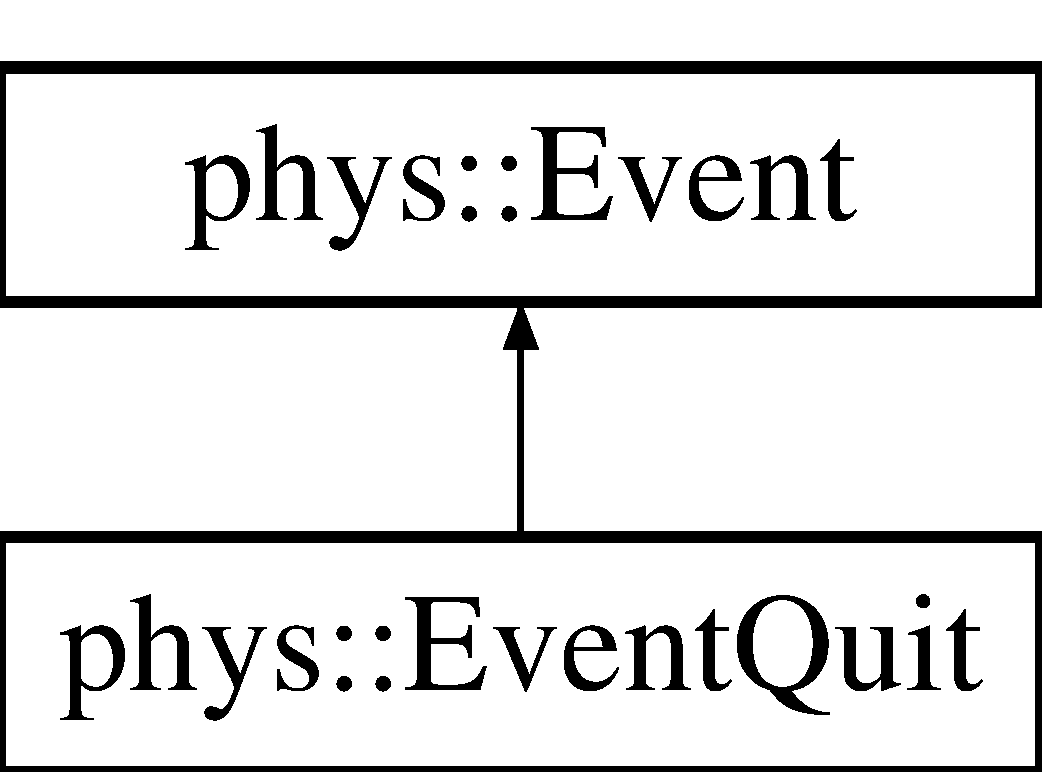
\includegraphics[height=2.000000cm]{dd/dea/classphys_1_1EventQuit}
\end{center}
\end{figure}
\subsection*{Public Member Functions}
\begin{DoxyCompactItemize}
\item 
virtual \hyperlink{classphys_1_1EventBase_a5e6a8564e127f654123f0bf6a2751923}{EventType} \hyperlink{classphys_1_1EventQuit_a3bfca875349e73dbda47c3c62a253e3b}{GetType} () const 
\begin{DoxyCompactList}\small\item\em This returns EventType::QuitMessage. \item\end{DoxyCompactList}\end{DoxyCompactItemize}


\subsection{Detailed Description}
This is intended to convey the message that quitting needs to happen. This stores not data other than the fact that this is a Quit event. This means that either an underlying system like the OS or a service has requested a quit, or the application has manually put a quit message in the queue to signal that a graceful shutdown needs to occur. 

Definition at line 63 of file eventquit.h.



\subsection{Member Function Documentation}
\hypertarget{classphys_1_1EventQuit_a3bfca875349e73dbda47c3c62a253e3b}{
\index{phys::EventQuit@{phys::EventQuit}!GetType@{GetType}}
\index{GetType@{GetType}!phys::EventQuit@{phys::EventQuit}}
\subsubsection[{GetType}]{\setlength{\rightskip}{0pt plus 5cm}{\bf EventBase::EventType} phys::EventQuit::GetType (
\begin{DoxyParamCaption}
{}
\end{DoxyParamCaption}
) const\hspace{0.3cm}{\ttfamily  \mbox{[}virtual\mbox{]}}}}
\label{dd/dea/classphys_1_1EventQuit_a3bfca875349e73dbda47c3c62a253e3b}


This returns EventType::QuitMessage. 

This returns the kind of message this is, specifcally EventType::QuitMessage . If this functions returns EventType::QuitMessage, then and event pointer can safely be cast to \hyperlink{classphys_1_1EventQuit}{phys::EventQuit} . This method is inherited from phys::Event . 

Implements \hyperlink{classphys_1_1EventBase_a1b3d29b6ecf30f18cc3e1825a515c508}{phys::EventBase}.



Definition at line 52 of file eventquit.cpp.



The documentation for this class was generated from the following files:\begin{DoxyCompactItemize}
\item 
eventquit.h\item 
eventquit.cpp\end{DoxyCompactItemize}

\hypertarget{classphys_1_1EventRenderTime}{
\section{phys::EventRenderTime Class Reference}
\label{d3/d8b/classphys_1_1EventRenderTime}\index{phys::EventRenderTime@{phys::EventRenderTime}}
}


This communicates the amount of time since the world was rendered.  




{\ttfamily \#include $<$eventrendertime.h$>$}

Inheritance diagram for phys::EventRenderTime:\begin{figure}[H]
\begin{center}
\leavevmode
\includegraphics[height=2cm]{d3/d8b/classphys_1_1EventRenderTime}
\end{center}
\end{figure}
\subsection*{Public Member Functions}
\begin{DoxyCompactItemize}
\item 
\hyperlink{classphys_1_1EventRenderTime_af2384f7b09bbea42dcd2539a9e1747fd}{EventRenderTime} (Whole Milliseconds)
\begin{DoxyCompactList}\small\item\em The Constructor. \item\end{DoxyCompactList}\item 
virtual \hyperlink{classphys_1_1Event_af5fdbb3e08d8e578d58770fbc606fda7}{EventType} \hyperlink{classphys_1_1EventRenderTime_a66918bf3793196899621e4442a6f7a57}{getEventType} () const 
\begin{DoxyCompactList}\small\item\em Returns that this event is a EventType::RenderTime. \item\end{DoxyCompactList}\item 
Whole \hyperlink{classphys_1_1EventRenderTime_ac9f20f13bf1f6e542151be2ce8ea2fa4}{getMilliSecondsSinceLastFrame} ()
\begin{DoxyCompactList}\small\item\em Returns the a floating point value with the amount of time. \item\end{DoxyCompactList}\end{DoxyCompactItemize}


\subsection{Detailed Description}
This communicates the amount of time since the world was rendered. This stores in milliseconds the amount of time since the last rendering of the world. 

Definition at line 59 of file eventrendertime.h.



\subsection{Constructor \& Destructor Documentation}
\hypertarget{classphys_1_1EventRenderTime_af2384f7b09bbea42dcd2539a9e1747fd}{
\index{phys::EventRenderTime@{phys::EventRenderTime}!EventRenderTime@{EventRenderTime}}
\index{EventRenderTime@{EventRenderTime}!phys::EventRenderTime@{phys::EventRenderTime}}
\subsubsection[{EventRenderTime}]{\setlength{\rightskip}{0pt plus 5cm}phys::EventRenderTime::EventRenderTime (Whole {\em Milliseconds})}}
\label{d3/d8b/classphys_1_1EventRenderTime_af2384f7b09bbea42dcd2539a9e1747fd}


The Constructor. 

This is the only way to set the time 
\begin{DoxyParams}{Parameters}
\item[{\em Milliseconds}]As it says, the amount of milliseconds since the last rendering \end{DoxyParams}


Definition at line 53 of file eventrendertime.cpp.



\subsection{Member Function Documentation}
\hypertarget{classphys_1_1EventRenderTime_a66918bf3793196899621e4442a6f7a57}{
\index{phys::EventRenderTime@{phys::EventRenderTime}!getEventType@{getEventType}}
\index{getEventType@{getEventType}!phys::EventRenderTime@{phys::EventRenderTime}}
\subsubsection[{getEventType}]{\setlength{\rightskip}{0pt plus 5cm}{\bf Event::EventType} phys::EventRenderTime::getEventType () const\hspace{0.3cm}{\ttfamily  \mbox{[}virtual\mbox{]}}}}
\label{d3/d8b/classphys_1_1EventRenderTime_a66918bf3793196899621e4442a6f7a57}


Returns that this event is a EventType::RenderTime. 

This is primarily for the benefit of sorting thorugh event pointers. If this functions returns EventType::RenderTime, then and event pointer can safely be cast to \hyperlink{classphys_1_1EventRenderTime}{phys::EventRenderTime} . This method is inherited from \hyperlink{classphys_1_1Event}{phys::Event} . 

Implements \hyperlink{classphys_1_1Event_ac2c0623a6bc399e62f4b9fb2c022ea73}{phys::Event}.



Definition at line 58 of file eventrendertime.cpp.

\hypertarget{classphys_1_1EventRenderTime_ac9f20f13bf1f6e542151be2ce8ea2fa4}{
\index{phys::EventRenderTime@{phys::EventRenderTime}!getMilliSecondsSinceLastFrame@{getMilliSecondsSinceLastFrame}}
\index{getMilliSecondsSinceLastFrame@{getMilliSecondsSinceLastFrame}!phys::EventRenderTime@{phys::EventRenderTime}}
\subsubsection[{getMilliSecondsSinceLastFrame}]{\setlength{\rightskip}{0pt plus 5cm}Whole phys::EventRenderTime::getMilliSecondsSinceLastFrame ()}}
\label{d3/d8b/classphys_1_1EventRenderTime_ac9f20f13bf1f6e542151be2ce8ea2fa4}


Returns the a floating point value with the amount of time. 

Returns the a floating point value with the amount of time. \begin{DoxyReturn}{Returns}
A floating point value with the amount of time. 
\end{DoxyReturn}


Definition at line 63 of file eventrendertime.cpp.



The documentation for this class was generated from the following files:\begin{DoxyCompactItemize}
\item 
eventrendertime.h\item 
eventrendertime.cpp\end{DoxyCompactItemize}

\hypertarget{classphys_1_1GraphicsSettings}{
\section{phys::GraphicsSettings Class Reference}
\label{dc/df1/classphys_1_1GraphicsSettings}\index{phys::GraphicsSettings@{phys::GraphicsSettings}}
}


This is intended to store basic graphics setting for the user.  




{\ttfamily \#include $<$graphicsettings.h$>$}

\subsection*{Public Member Functions}
\begin{DoxyCompactItemize}
\item 
\hyperlink{classphys_1_1GraphicsSettings_aceaaf53585413067adbf271e2c1e48fa}{GraphicsSettings} ()
\begin{DoxyCompactList}\small\item\em Default constructor. \item\end{DoxyCompactList}\item 
\hyperlink{classphys_1_1GraphicsSettings_a7cbb84f41101ef66a04e2a0990f796a2}{GraphicsSettings} (const \hyperlink{namespacephys_a460f6bc24c8dd347b05e0366ae34f34a}{Whole} \&Width\_\-, const \hyperlink{namespacephys_a460f6bc24c8dd347b05e0366ae34f34a}{Whole} \&Height\_\-, const bool \&FullScreen\_\-)
\begin{DoxyCompactList}\small\item\em Versatile Constructor. \item\end{DoxyCompactList}\item 
void \hyperlink{classphys_1_1GraphicsSettings_a63d41a500ee1ddf0ea9ffba5e353bae0}{Construct} (const \hyperlink{namespacephys_a460f6bc24c8dd347b05e0366ae34f34a}{Whole} \&Width\_\-, const \hyperlink{namespacephys_a460f6bc24c8dd347b05e0366ae34f34a}{Whole} \&Height\_\-, const bool \&FullScreen\_\-)
\begin{DoxyCompactList}\small\item\em Adjust all Settings. \item\end{DoxyCompactList}\item 
bool \hyperlink{classphys_1_1GraphicsSettings_a8871ea7d5c65c3b59d1d34b59531743f}{getFullscreen} () const 
\begin{DoxyCompactList}\small\item\em Gets the Fullscreen Setting. \item\end{DoxyCompactList}\item 
void \hyperlink{classphys_1_1GraphicsSettings_aba9e127ab2cf3f20604313e39d32f7a8}{setFullscreen} (const bool \&Fullscreen\_\-)
\begin{DoxyCompactList}\small\item\em Set the Fullscreen Setting. \item\end{DoxyCompactList}\item 
\hyperlink{namespacephys_a460f6bc24c8dd347b05e0366ae34f34a}{Whole} \hyperlink{classphys_1_1GraphicsSettings_a118171db4fc0a2b17da4284cc91fbeb4}{getRenderHeight} () const 
\begin{DoxyCompactList}\small\item\em Gets the Height of the Rendering Area. \item\end{DoxyCompactList}\item 
void \hyperlink{classphys_1_1GraphicsSettings_a1e6b11740f681beb4d64553656a760f1}{setRenderHeight} (const \hyperlink{namespacephys_a460f6bc24c8dd347b05e0366ae34f34a}{Whole} \&Height\_\-)
\begin{DoxyCompactList}\small\item\em Sets the Height. \item\end{DoxyCompactList}\item 
\hyperlink{namespacephys_a460f6bc24c8dd347b05e0366ae34f34a}{Whole} \hyperlink{classphys_1_1GraphicsSettings_aa8a8548afca8d3e127a1be69a2c1eba2}{getRenderWidth} () const 
\begin{DoxyCompactList}\small\item\em Gets the Width of the Rendering Area. \item\end{DoxyCompactList}\item 
void \hyperlink{classphys_1_1GraphicsSettings_a7cebb39f829f5e600231b4efc22b9ec3}{setRenderWidth} (const \hyperlink{namespacephys_a460f6bc24c8dd347b05e0366ae34f34a}{Whole} \&Width\_\-)
\begin{DoxyCompactList}\small\item\em Sets the Width. \item\end{DoxyCompactList}\end{DoxyCompactItemize}


\subsection{Detailed Description}
This is intended to store basic graphics setting for the user. This stores x/y resolution, fullscreen and in the future other settings. This is intended to make it easy for developers to pass/move around complex graphics settings. We hope to eventually include other items like shader settings, rendering API, and maybe other settings too. 

Definition at line 53 of file graphicsettings.h.



\subsection{Constructor \& Destructor Documentation}
\hypertarget{classphys_1_1GraphicsSettings_aceaaf53585413067adbf271e2c1e48fa}{
\index{phys::GraphicsSettings@{phys::GraphicsSettings}!GraphicsSettings@{GraphicsSettings}}
\index{GraphicsSettings@{GraphicsSettings}!phys::GraphicsSettings@{phys::GraphicsSettings}}
\subsubsection[{GraphicsSettings}]{\setlength{\rightskip}{0pt plus 5cm}phys::GraphicsSettings::GraphicsSettings ()}}
\label{dc/df1/classphys_1_1GraphicsSettings_aceaaf53585413067adbf271e2c1e48fa}


Default constructor. 

This creates a default Graphics Settings with resolution 640x480 with fullscreen set to false 

Definition at line 51 of file graphicsettings.cpp.

\hypertarget{classphys_1_1GraphicsSettings_a7cbb84f41101ef66a04e2a0990f796a2}{
\index{phys::GraphicsSettings@{phys::GraphicsSettings}!GraphicsSettings@{GraphicsSettings}}
\index{GraphicsSettings@{GraphicsSettings}!phys::GraphicsSettings@{phys::GraphicsSettings}}
\subsubsection[{GraphicsSettings}]{\setlength{\rightskip}{0pt plus 5cm}phys::GraphicsSettings::GraphicsSettings (const {\bf Whole} \& {\em Width\_\-}, \/  const {\bf Whole} \& {\em Height\_\-}, \/  const bool \& {\em FullScreen\_\-})}}
\label{dc/df1/classphys_1_1GraphicsSettings_a7cbb84f41101ef66a04e2a0990f796a2}


Versatile Constructor. 


\begin{DoxyParams}{Parameters}
\item[{\em Width\_\-}]The desired width. \item[{\em Height\_\-}]The desired height. \item[{\em FullScreen\_\-}]True if fullscreen, false if not.\end{DoxyParams}
This creates a Graphics Settings with resolution and fullscreen passed into to it. Be careful that the settings selected are appropriate. Many mobile devices do not support windows, and many screens do not support arbitrary resolutions in fullscreen mode. 

Definition at line 56 of file graphicsettings.cpp.



\subsection{Member Function Documentation}
\hypertarget{classphys_1_1GraphicsSettings_a63d41a500ee1ddf0ea9ffba5e353bae0}{
\index{phys::GraphicsSettings@{phys::GraphicsSettings}!Construct@{Construct}}
\index{Construct@{Construct}!phys::GraphicsSettings@{phys::GraphicsSettings}}
\subsubsection[{Construct}]{\setlength{\rightskip}{0pt plus 5cm}void phys::GraphicsSettings::Construct (const {\bf Whole} \& {\em Width\_\-}, \/  const {\bf Whole} \& {\em Height\_\-}, \/  const bool \& {\em FullScreen\_\-})}}
\label{dc/df1/classphys_1_1GraphicsSettings_a63d41a500ee1ddf0ea9ffba5e353bae0}


Adjust all Settings. 


\begin{DoxyParams}{Parameters}
\item[{\em Width\_\-}]The desired width. \item[{\em Height\_\-}]The desired height. \item[{\em FullScreen\_\-}]True if fullscreen, false if not.\end{DoxyParams}
This adjusts most data in this Graphics Settings and accepts new resolution and fullscreen settings. Be careful that the settings selected are appropriate. Many mobile devices do not support windows, and many screens do not support arbitrary resolutions in fullscreen mode. 

Definition at line 61 of file graphicsettings.cpp.

\hypertarget{classphys_1_1GraphicsSettings_a8871ea7d5c65c3b59d1d34b59531743f}{
\index{phys::GraphicsSettings@{phys::GraphicsSettings}!getFullscreen@{getFullscreen}}
\index{getFullscreen@{getFullscreen}!phys::GraphicsSettings@{phys::GraphicsSettings}}
\subsubsection[{getFullscreen}]{\setlength{\rightskip}{0pt plus 5cm}bool phys::GraphicsSettings::getFullscreen () const}}
\label{dc/df1/classphys_1_1GraphicsSettings_a8871ea7d5c65c3b59d1d34b59531743f}


Gets the Fullscreen Setting. 

Gets the Fullscreen Setting \begin{DoxyReturn}{Returns}
This returns a bool, true if fullscreen is set, false otherwise 
\end{DoxyReturn}


Definition at line 72 of file graphicsettings.cpp.

\hypertarget{classphys_1_1GraphicsSettings_a118171db4fc0a2b17da4284cc91fbeb4}{
\index{phys::GraphicsSettings@{phys::GraphicsSettings}!getRenderHeight@{getRenderHeight}}
\index{getRenderHeight@{getRenderHeight}!phys::GraphicsSettings@{phys::GraphicsSettings}}
\subsubsection[{getRenderHeight}]{\setlength{\rightskip}{0pt plus 5cm}{\bf Whole} phys::GraphicsSettings::getRenderHeight () const}}
\label{dc/df1/classphys_1_1GraphicsSettings_a118171db4fc0a2b17da4284cc91fbeb4}


Gets the Height of the Rendering Area. 

Gets the Height of the Rendering Area \begin{DoxyReturn}{Returns}
This returns the Height of the Rendering Area 
\end{DoxyReturn}


Definition at line 87 of file graphicsettings.cpp.

\hypertarget{classphys_1_1GraphicsSettings_aa8a8548afca8d3e127a1be69a2c1eba2}{
\index{phys::GraphicsSettings@{phys::GraphicsSettings}!getRenderWidth@{getRenderWidth}}
\index{getRenderWidth@{getRenderWidth}!phys::GraphicsSettings@{phys::GraphicsSettings}}
\subsubsection[{getRenderWidth}]{\setlength{\rightskip}{0pt plus 5cm}{\bf Whole} phys::GraphicsSettings::getRenderWidth () const}}
\label{dc/df1/classphys_1_1GraphicsSettings_aa8a8548afca8d3e127a1be69a2c1eba2}


Gets the Width of the Rendering Area. 

Gets the Width of the Rendering Area \begin{DoxyReturn}{Returns}
This returns the Width of the Rendering Area 
\end{DoxyReturn}


Definition at line 92 of file graphicsettings.cpp.

\hypertarget{classphys_1_1GraphicsSettings_aba9e127ab2cf3f20604313e39d32f7a8}{
\index{phys::GraphicsSettings@{phys::GraphicsSettings}!setFullscreen@{setFullscreen}}
\index{setFullscreen@{setFullscreen}!phys::GraphicsSettings@{phys::GraphicsSettings}}
\subsubsection[{setFullscreen}]{\setlength{\rightskip}{0pt plus 5cm}void phys::GraphicsSettings::setFullscreen (const bool \& {\em Fullscreen\_\-})}}
\label{dc/df1/classphys_1_1GraphicsSettings_aba9e127ab2cf3f20604313e39d32f7a8}


Set the Fullscreen Setting. 

Set the Fullscreen Setting 
\begin{DoxyParams}{Parameters}
\item[{\em Fullscreen\_\-}]This accepts a bool. True for fullscreen, false for windowed \end{DoxyParams}


\begin{Desc}
\item[\hyperlink{todo__todo000009}{Todo}]TODO: We really should double check that going into fullscreen worked the way we wanted, this fails in too many games \end{Desc}




Definition at line 78 of file graphicsettings.cpp.

\hypertarget{classphys_1_1GraphicsSettings_a1e6b11740f681beb4d64553656a760f1}{
\index{phys::GraphicsSettings@{phys::GraphicsSettings}!setRenderHeight@{setRenderHeight}}
\index{setRenderHeight@{setRenderHeight}!phys::GraphicsSettings@{phys::GraphicsSettings}}
\subsubsection[{setRenderHeight}]{\setlength{\rightskip}{0pt plus 5cm}void phys::GraphicsSettings::setRenderHeight (const {\bf Whole} \& {\em Height\_\-})}}
\label{dc/df1/classphys_1_1GraphicsSettings_a1e6b11740f681beb4d64553656a760f1}


Sets the Height. 

Set the Render Height inside the window in windowed mode, set the resolution of the screen in fullscreen 
\begin{DoxyParams}{Parameters}
\item[{\em Height\_\-}]This accepts a Whole. \end{DoxyParams}


Definition at line 97 of file graphicsettings.cpp.

\hypertarget{classphys_1_1GraphicsSettings_a7cebb39f829f5e600231b4efc22b9ec3}{
\index{phys::GraphicsSettings@{phys::GraphicsSettings}!setRenderWidth@{setRenderWidth}}
\index{setRenderWidth@{setRenderWidth}!phys::GraphicsSettings@{phys::GraphicsSettings}}
\subsubsection[{setRenderWidth}]{\setlength{\rightskip}{0pt plus 5cm}void phys::GraphicsSettings::setRenderWidth (const {\bf Whole} \& {\em Width\_\-})}}
\label{dc/df1/classphys_1_1GraphicsSettings_a7cebb39f829f5e600231b4efc22b9ec3}


Sets the Width. 

Set the Render Width inside the window in windowed mode, set the resolution of the screen in fullscreen 
\begin{DoxyParams}{Parameters}
\item[{\em Width\_\-}]This accepts a Whole. \end{DoxyParams}


Definition at line 102 of file graphicsettings.cpp.



The documentation for this class was generated from the following files:\begin{DoxyCompactItemize}
\item 
graphicsettings.h\item 
graphicsettings.cpp\end{DoxyCompactItemize}

\hypertarget{classphys_1_1MetaCode}{
\section{phys::MetaCode Class Reference}
\label{da/dc9/classphys_1_1MetaCode}\index{phys::MetaCode@{phys::MetaCode}}
}


This Determines the kind of user input.  




{\ttfamily \#include $<$metacode.h$>$}

\subsection*{Public Types}
\begin{DoxyCompactItemize}
\item 
enum \hyperlink{classphys_1_1MetaCode_a3e501cbb5bf0f6f1fdb7211465bda8d8}{InputCode} \{ \par
\hyperlink{classphys_1_1MetaCode_a3e501cbb5bf0f6f1fdb7211465bda8d8a061a36c9b5d9661314fd9d276b33042f}{KEY\_\-UNKNOWN} =  0, 
\hyperlink{classphys_1_1MetaCode_a3e501cbb5bf0f6f1fdb7211465bda8d8a45d7f3824a440f5bea5e616a6d6ea0b5}{KEY\_\-FIRST} =  0, 
{\bfseries KEY\_\-BACKSPACE} =  8, 
{\bfseries KEY\_\-TAB} =  9, 
\par
{\bfseries KEY\_\-CLEAR} =  12, 
{\bfseries KEY\_\-RETURN} =  13, 
{\bfseries KEY\_\-PAUSE} =  19, 
{\bfseries KEY\_\-ESCAPE} =  27, 
\par
{\bfseries KEY\_\-SPACE} =  32, 
{\bfseries KEY\_\-EXCLAIM} =  33, 
{\bfseries KEY\_\-QUOTEDBL} =  34, 
{\bfseries KEY\_\-HASH} =  35, 
\par
{\bfseries KEY\_\-DOLLAR} =  36, 
{\bfseries KEY\_\-AMPERSAND} =  38, 
{\bfseries KEY\_\-QUOTE} =  39, 
{\bfseries KEY\_\-LEFTPAREN} =  40, 
\par
{\bfseries KEY\_\-RIGHTPAREN} =  41, 
{\bfseries KEY\_\-ASTERISK} =  42, 
{\bfseries KEY\_\-PLUS} =  43, 
{\bfseries KEY\_\-COMMA} =  44, 
\par
{\bfseries KEY\_\-MINUS} =  45, 
{\bfseries KEY\_\-PERIOD} =  46, 
{\bfseries KEY\_\-SLASH} =  47, 
{\bfseries KEY\_\-0} =  48, 
\par
{\bfseries KEY\_\-1} =  49, 
{\bfseries KEY\_\-2} =  50, 
{\bfseries KEY\_\-3} =  51, 
{\bfseries KEY\_\-4} =  52, 
\par
{\bfseries KEY\_\-5} =  53, 
{\bfseries KEY\_\-6} =  54, 
{\bfseries KEY\_\-7} =  55, 
{\bfseries KEY\_\-8} =  56, 
\par
{\bfseries KEY\_\-9} =  57, 
{\bfseries KEY\_\-COLON} =  58, 
{\bfseries KEY\_\-SEMICOLON} =  59, 
{\bfseries KEY\_\-LESS} =  60, 
\par
{\bfseries KEY\_\-EQUALS} =  61, 
{\bfseries KEY\_\-GREATER} =  62, 
{\bfseries KEY\_\-QUESTION} =  63, 
{\bfseries KEY\_\-AT} =  64, 
\par
{\bfseries KEY\_\-LEFTBRACKET} =  91, 
{\bfseries KEY\_\-BACKSLASH} =  92, 
{\bfseries KEY\_\-RIGHTBRACKET} =  93, 
{\bfseries KEY\_\-CARET} =  94, 
\par
{\bfseries KEY\_\-UNDERSCORE} =  95, 
{\bfseries KEY\_\-BACKQUOTE} =  96, 
{\bfseries KEY\_\-a} =  97, 
{\bfseries KEY\_\-b} =  98, 
\par
{\bfseries KEY\_\-c} =  99, 
{\bfseries KEY\_\-d} =  100, 
{\bfseries KEY\_\-e} =  101, 
{\bfseries KEY\_\-f} =  102, 
\par
{\bfseries KEY\_\-g} =  103, 
{\bfseries KEY\_\-h} =  104, 
{\bfseries KEY\_\-i} =  105, 
{\bfseries KEY\_\-j} =  106, 
\par
{\bfseries KEY\_\-k} =  107, 
{\bfseries KEY\_\-l} =  108, 
{\bfseries KEY\_\-m} =  109, 
{\bfseries KEY\_\-n} =  110, 
\par
{\bfseries KEY\_\-o} =  111, 
{\bfseries KEY\_\-p} =  112, 
{\bfseries KEY\_\-q} =  113, 
{\bfseries KEY\_\-r} =  114, 
\par
{\bfseries KEY\_\-s} =  115, 
{\bfseries KEY\_\-t} =  116, 
{\bfseries KEY\_\-u} =  117, 
{\bfseries KEY\_\-v} =  118, 
\par
{\bfseries KEY\_\-w} =  119, 
{\bfseries KEY\_\-x} =  120, 
{\bfseries KEY\_\-y} =  121, 
{\bfseries KEY\_\-z} =  122, 
\par
{\bfseries KEY\_\-DELETE} =  127, 
{\bfseries KEY\_\-WORLD\_\-0} =  160, 
{\bfseries KEY\_\-WORLD\_\-1} =  161, 
{\bfseries KEY\_\-WORLD\_\-2} =  162, 
\par
{\bfseries KEY\_\-WORLD\_\-3} =  163, 
{\bfseries KEY\_\-WORLD\_\-4} =  164, 
{\bfseries KEY\_\-WORLD\_\-5} =  165, 
{\bfseries KEY\_\-WORLD\_\-6} =  166, 
\par
{\bfseries KEY\_\-WORLD\_\-7} =  167, 
{\bfseries KEY\_\-WORLD\_\-8} =  168, 
{\bfseries KEY\_\-WORLD\_\-9} =  169, 
{\bfseries KEY\_\-WORLD\_\-10} =  170, 
\par
{\bfseries KEY\_\-WORLD\_\-11} =  171, 
{\bfseries KEY\_\-WORLD\_\-12} =  172, 
{\bfseries KEY\_\-WORLD\_\-13} =  173, 
{\bfseries KEY\_\-WORLD\_\-14} =  174, 
\par
{\bfseries KEY\_\-WORLD\_\-15} =  175, 
{\bfseries KEY\_\-WORLD\_\-16} =  176, 
{\bfseries KEY\_\-WORLD\_\-17} =  177, 
{\bfseries KEY\_\-WORLD\_\-18} =  178, 
\par
{\bfseries KEY\_\-WORLD\_\-19} =  179, 
{\bfseries KEY\_\-WORLD\_\-20} =  180, 
{\bfseries KEY\_\-WORLD\_\-21} =  181, 
{\bfseries KEY\_\-WORLD\_\-22} =  182, 
\par
{\bfseries KEY\_\-WORLD\_\-23} =  183, 
{\bfseries KEY\_\-WORLD\_\-24} =  184, 
{\bfseries KEY\_\-WORLD\_\-25} =  185, 
{\bfseries KEY\_\-WORLD\_\-26} =  186, 
\par
{\bfseries KEY\_\-WORLD\_\-27} =  187, 
{\bfseries KEY\_\-WORLD\_\-28} =  188, 
{\bfseries KEY\_\-WORLD\_\-29} =  189, 
{\bfseries KEY\_\-WORLD\_\-30} =  190, 
\par
{\bfseries KEY\_\-WORLD\_\-31} =  191, 
{\bfseries KEY\_\-WORLD\_\-32} =  192, 
{\bfseries KEY\_\-WORLD\_\-33} =  193, 
{\bfseries KEY\_\-WORLD\_\-34} =  194, 
\par
{\bfseries KEY\_\-WORLD\_\-35} =  195, 
{\bfseries KEY\_\-WORLD\_\-36} =  196, 
{\bfseries KEY\_\-WORLD\_\-37} =  197, 
{\bfseries KEY\_\-WORLD\_\-38} =  198, 
\par
{\bfseries KEY\_\-WORLD\_\-39} =  199, 
{\bfseries KEY\_\-WORLD\_\-40} =  200, 
{\bfseries KEY\_\-WORLD\_\-41} =  201, 
{\bfseries KEY\_\-WORLD\_\-42} =  202, 
\par
{\bfseries KEY\_\-WORLD\_\-43} =  203, 
{\bfseries KEY\_\-WORLD\_\-44} =  204, 
{\bfseries KEY\_\-WORLD\_\-45} =  205, 
{\bfseries KEY\_\-WORLD\_\-46} =  206, 
\par
{\bfseries KEY\_\-WORLD\_\-47} =  207, 
{\bfseries KEY\_\-WORLD\_\-48} =  208, 
{\bfseries KEY\_\-WORLD\_\-49} =  209, 
{\bfseries KEY\_\-WORLD\_\-50} =  210, 
\par
{\bfseries KEY\_\-WORLD\_\-51} =  211, 
{\bfseries KEY\_\-WORLD\_\-52} =  212, 
{\bfseries KEY\_\-WORLD\_\-53} =  213, 
{\bfseries KEY\_\-WORLD\_\-54} =  214, 
\par
{\bfseries KEY\_\-WORLD\_\-55} =  215, 
{\bfseries KEY\_\-WORLD\_\-56} =  216, 
{\bfseries KEY\_\-WORLD\_\-57} =  217, 
{\bfseries KEY\_\-WORLD\_\-58} =  218, 
\par
{\bfseries KEY\_\-WORLD\_\-59} =  219, 
{\bfseries KEY\_\-WORLD\_\-60} =  220, 
{\bfseries KEY\_\-WORLD\_\-61} =  221, 
{\bfseries KEY\_\-WORLD\_\-62} =  222, 
\par
{\bfseries KEY\_\-WORLD\_\-63} =  223, 
{\bfseries KEY\_\-WORLD\_\-64} =  224, 
{\bfseries KEY\_\-WORLD\_\-65} =  225, 
{\bfseries KEY\_\-WORLD\_\-66} =  226, 
\par
{\bfseries KEY\_\-WORLD\_\-67} =  227, 
{\bfseries KEY\_\-WORLD\_\-68} =  228, 
{\bfseries KEY\_\-WORLD\_\-69} =  229, 
{\bfseries KEY\_\-WORLD\_\-70} =  230, 
\par
{\bfseries KEY\_\-WORLD\_\-71} =  231, 
{\bfseries KEY\_\-WORLD\_\-72} =  232, 
{\bfseries KEY\_\-WORLD\_\-73} =  233, 
{\bfseries KEY\_\-WORLD\_\-74} =  234, 
\par
{\bfseries KEY\_\-WORLD\_\-75} =  235, 
{\bfseries KEY\_\-WORLD\_\-76} =  236, 
{\bfseries KEY\_\-WORLD\_\-77} =  237, 
{\bfseries KEY\_\-WORLD\_\-78} =  238, 
\par
{\bfseries KEY\_\-WORLD\_\-79} =  239, 
{\bfseries KEY\_\-WORLD\_\-80} =  240, 
{\bfseries KEY\_\-WORLD\_\-81} =  241, 
{\bfseries KEY\_\-WORLD\_\-82} =  242, 
\par
{\bfseries KEY\_\-WORLD\_\-83} =  243, 
{\bfseries KEY\_\-WORLD\_\-84} =  244, 
{\bfseries KEY\_\-WORLD\_\-85} =  245, 
{\bfseries KEY\_\-WORLD\_\-86} =  246, 
\par
{\bfseries KEY\_\-WORLD\_\-87} =  247, 
{\bfseries KEY\_\-WORLD\_\-88} =  248, 
{\bfseries KEY\_\-WORLD\_\-89} =  249, 
{\bfseries KEY\_\-WORLD\_\-90} =  250, 
\par
{\bfseries KEY\_\-WORLD\_\-91} =  251, 
{\bfseries KEY\_\-WORLD\_\-92} =  252, 
{\bfseries KEY\_\-WORLD\_\-93} =  253, 
{\bfseries KEY\_\-WORLD\_\-94} =  254, 
\par
{\bfseries KEY\_\-WORLD\_\-95} =  255, 
{\bfseries KEY\_\-KP0} =  256, 
{\bfseries KEY\_\-KP1} =  257, 
{\bfseries KEY\_\-KP2} =  258, 
\par
{\bfseries KEY\_\-KP3} =  259, 
{\bfseries KEY\_\-KP4} =  260, 
{\bfseries KEY\_\-KP5} =  261, 
{\bfseries KEY\_\-KP6} =  262, 
\par
{\bfseries KEY\_\-KP7} =  263, 
{\bfseries KEY\_\-KP8} =  264, 
{\bfseries KEY\_\-KP9} =  265, 
{\bfseries KEY\_\-KP\_\-PERIOD} =  266, 
\par
{\bfseries KEY\_\-KP\_\-DIVIDE} =  267, 
{\bfseries KEY\_\-KP\_\-MULTIPLY} =  268, 
{\bfseries KEY\_\-KP\_\-MINUS} =  269, 
{\bfseries KEY\_\-KP\_\-PLUS} =  270, 
\par
{\bfseries KEY\_\-KP\_\-ENTER} =  271, 
{\bfseries KEY\_\-KP\_\-EQUALS} =  272, 
{\bfseries KEY\_\-UP} =  273, 
{\bfseries KEY\_\-DOWN} =  274, 
\par
{\bfseries KEY\_\-RIGHT} =  275, 
{\bfseries KEY\_\-LEFT} =  276, 
{\bfseries KEY\_\-INSERT} =  277, 
{\bfseries KEY\_\-HOME} =  278, 
\par
{\bfseries KEY\_\-END} =  279, 
{\bfseries KEY\_\-PAGEUP} =  280, 
{\bfseries KEY\_\-PAGEDOWN} =  281, 
{\bfseries KEY\_\-F1} =  282, 
\par
{\bfseries KEY\_\-F2} =  283, 
{\bfseries KEY\_\-F3} =  284, 
{\bfseries KEY\_\-F4} =  285, 
{\bfseries KEY\_\-F5} =  286, 
\par
{\bfseries KEY\_\-F6} =  287, 
{\bfseries KEY\_\-F7} =  288, 
{\bfseries KEY\_\-F8} =  289, 
{\bfseries KEY\_\-F9} =  290, 
\par
{\bfseries KEY\_\-F10} =  291, 
{\bfseries KEY\_\-F11} =  292, 
{\bfseries KEY\_\-F12} =  293, 
{\bfseries KEY\_\-F13} =  294, 
\par
{\bfseries KEY\_\-F14} =  295, 
{\bfseries KEY\_\-F15} =  296, 
{\bfseries KEY\_\-NUMLOCK} =  300, 
{\bfseries KEY\_\-CAPSLOCK} =  301, 
\par
{\bfseries KEY\_\-SCROLLOCK} =  302, 
{\bfseries KEY\_\-RSHIFT} =  303, 
{\bfseries KEY\_\-LSHIFT} =  304, 
{\bfseries KEY\_\-RCTRL} =  305, 
\par
{\bfseries KEY\_\-LCTRL} =  306, 
{\bfseries KEY\_\-RALT} =  307, 
{\bfseries KEY\_\-LALT} =  308, 
{\bfseries KEY\_\-RMETA} =  309, 
\par
{\bfseries KEY\_\-LMETA} =  310, 
\hyperlink{classphys_1_1MetaCode_a3e501cbb5bf0f6f1fdb7211465bda8d8aab77afaba4fc97faa9b9fe40d3a9ebbb}{KEY\_\-LSUPER} =  311, 
\hyperlink{classphys_1_1MetaCode_a3e501cbb5bf0f6f1fdb7211465bda8d8a84e2235ece031f83821867486ff52149}{KEY\_\-RSUPER} =  312, 
\hyperlink{classphys_1_1MetaCode_a3e501cbb5bf0f6f1fdb7211465bda8d8a9e26ea2006e876ccaa80fe4ae441da46}{KEY\_\-MODE} =  313, 
\par
\hyperlink{classphys_1_1MetaCode_a3e501cbb5bf0f6f1fdb7211465bda8d8aae92d5418d0273c8b43cb11f5e251a20}{KEY\_\-COMPOSE} =  314, 
{\bfseries KEY\_\-HELP} =  315, 
{\bfseries KEY\_\-PRINT} =  316, 
{\bfseries KEY\_\-SYSREQ} =  317, 
\par
{\bfseries KEY\_\-BREAK} =  318, 
{\bfseries KEY\_\-MENU} =  319, 
\hyperlink{classphys_1_1MetaCode_a3e501cbb5bf0f6f1fdb7211465bda8d8a08a2d04e3a40d746b81913e92a25a038}{KEY\_\-POWER} =  320, 
\hyperlink{classphys_1_1MetaCode_a3e501cbb5bf0f6f1fdb7211465bda8d8aee70075958d1650a7b48ba507103ec0c}{KEY\_\-EURO} =  321, 
\par
\hyperlink{classphys_1_1MetaCode_a3e501cbb5bf0f6f1fdb7211465bda8d8a15aabd8c4e36284ec057fafbda0d120a}{KEY\_\-UNDO} =  322, 
{\bfseries KEYMOD\_\-NONE} =  323, 
{\bfseries KEYMOD\_\-LSHIFT} =  324, 
{\bfseries KEYMOD\_\-RSHIFT} =  325, 
\par
{\bfseries KEYMOD\_\-LCTRL} =  326, 
{\bfseries KEYMOD\_\-RCTRL} =  327, 
{\bfseries KEYMOD\_\-LALT} =  328, 
{\bfseries KEYMOD\_\-RALT} =  329, 
\par
{\bfseries KEYMOD\_\-LMETA} =  330, 
{\bfseries KEYMOD\_\-RMETA} =  331, 
{\bfseries KEYMOD\_\-NUM} =  332, 
{\bfseries KEYMOD\_\-CAPS} =  333, 
\par
{\bfseries KEYMOD\_\-MODE} =  334, 
{\bfseries KEYMOD\_\-RESERVED} =  335, 
{\bfseries KEY\_\-LAST} =  379, 
\hyperlink{classphys_1_1MetaCode_a3e501cbb5bf0f6f1fdb7211465bda8d8a87685f9ca9462b329f2b86a17514f136}{INPUTEVENT\_\-FIRST} =  380, 
\par
\hyperlink{classphys_1_1MetaCode_a3e501cbb5bf0f6f1fdb7211465bda8d8a355649b334e903ada2496ad39dcd5f9d}{MOTION\_\-FIRST} =  460, 
\hyperlink{classphys_1_1MetaCode_a3e501cbb5bf0f6f1fdb7211465bda8d8a59cc92f5b2f42f7a138f8ea22e92d626}{MOTION\_\-LAST} =  469, 
\hyperlink{classphys_1_1MetaCode_a3e501cbb5bf0f6f1fdb7211465bda8d8acdb03d23d93022d5962db5026475b9c7}{MULTITOUCH\_\-FIRST} =  470, 
\hyperlink{classphys_1_1MetaCode_a3e501cbb5bf0f6f1fdb7211465bda8d8a94d804dc2330be620a8009252b5d5d22}{MULTITOUCH\_\-ACTION} =  471, 
\par
{\bfseries MULTITOUCH\_\-GESTURE} =  472, 
{\bfseries MULTITOUCH\_\-PINCH} =  473, 
{\bfseries MULTITOUCH\_\-STRETCH} =  474, 
{\bfseries MULTITOUCH\_\-LAST} =  479, 
\par
\hyperlink{classphys_1_1MetaCode_a3e501cbb5bf0f6f1fdb7211465bda8d8a1bb7f008c7d430e886141a3b8b697129}{MOUSE\_\-FIRST} =  480, 
\hyperlink{classphys_1_1MetaCode_a3e501cbb5bf0f6f1fdb7211465bda8d8a9cc80a2db206fb540fbb92a8ff64268a}{MOUSEBUTTON} =  481, 
{\bfseries MOUSEABSOLUTEVERTICAL} =  482, 
{\bfseries MOUSEABSOLUTEHORIZONTAL} =  483, 
\par
{\bfseries MOUSEVERTICAL} =  484, 
{\bfseries MOUSEHORIZONTAL} =  485, 
{\bfseries MOUSEWHEELVERTICAL} =  486, 
{\bfseries MOUSEWHEELHORIZONTAL} =  489, 
\par
{\bfseries MOUSE\_\-LAST} =  490, 
\hyperlink{classphys_1_1MetaCode_a3e501cbb5bf0f6f1fdb7211465bda8d8a666e564cae666de739b9b3cf047ec578}{JOYSTICK\_\-FIRST} =  499, 
\hyperlink{classphys_1_1MetaCode_a3e501cbb5bf0f6f1fdb7211465bda8d8aaaa2af6a60a9cd7403aa4786ef1ea389}{JOYSTICKBUTTON} =  500, 
{\bfseries JOYSTICKMOTIONAXIS} =  501, 
\par
{\bfseries JOYSTICKBALLVERTICAL} =  502, 
{\bfseries JOYSTICKBALLHORIZONTAL} =  503, 
{\bfseries JOYSTICKHATVERTICAL} =  504, 
{\bfseries JOYSTICKHATHORIZONTAL} =  505, 
\par
{\bfseries JOYSTICK\_\-LAST} =  506, 
\hyperlink{classphys_1_1MetaCode_a3e501cbb5bf0f6f1fdb7211465bda8d8adc78bfd04a85c4bbe39718f9acacbbe3}{INPUTEVENT\_\-LAST} =  512
 \}
\begin{DoxyCompactList}\small\item\em The InputCode enum defines all the posible types of inputs. \item\end{DoxyCompactList}\item 
enum \hyperlink{classphys_1_1MetaCode_a2fdfb26b3e50ceb0ccc60bfc4c3d6ac2}{ButtonState} \{ \hyperlink{classphys_1_1MetaCode_a2fdfb26b3e50ceb0ccc60bfc4c3d6ac2a6b5564408703517f36debd8c423e2dee}{BUTTON\_\-LIFTING} =  -\/1, 
\hyperlink{classphys_1_1MetaCode_a2fdfb26b3e50ceb0ccc60bfc4c3d6ac2ae275c52779b0f6ec37533af256a70cc3}{BUTTON\_\-UP} =  0, 
\hyperlink{classphys_1_1MetaCode_a2fdfb26b3e50ceb0ccc60bfc4c3d6ac2a33669b2b9ca814664296da55702e412d}{BUTTON\_\-PRESSING} =  1, 
\hyperlink{classphys_1_1MetaCode_a2fdfb26b3e50ceb0ccc60bfc4c3d6ac2a5b52ee1db94dbc2db23f3b4c267b5438}{BUTTON\_\-DOWN} =  2
 \}
\begin{DoxyCompactList}\small\item\em An Optional listing of value that can be used in a metacode to represent the information of a button press. \item\end{DoxyCompactList}\item 
enum \hyperlink{classphys_1_1MetaCode_af9ba277d1ef071be8861e35c2b7d82d6}{MouseWheelState} \{ \hyperlink{classphys_1_1MetaCode_af9ba277d1ef071be8861e35c2b7d82d6a15542262fc8fe9a3d6746f2b84ecde11}{MOUSEWHEEL\_\-UP} =  1, 
\hyperlink{classphys_1_1MetaCode_af9ba277d1ef071be8861e35c2b7d82d6aa3d86fe74d1c191d7c57f886c0b8d99a}{MOUSEWHEEL\_\-UNCHANGED} =  0, 
\hyperlink{classphys_1_1MetaCode_af9ba277d1ef071be8861e35c2b7d82d6ab6edd0886d2ec2d2917bbad96ce3d510}{MOUSEWHEEL\_\-DOWN} =  -\/1
 \}
\begin{DoxyCompactList}\small\item\em An Optional listing of values that can be used in a metacode Indicate spin of a mouse wheel. \item\end{DoxyCompactList}\end{DoxyCompactItemize}
\subsection*{Public Member Functions}
\begin{DoxyCompactItemize}
\item 
\hyperlink{classphys_1_1MetaCode_ae2c80c84f924ddfd880f46ffe6a1746e}{MetaCode} ()
\begin{DoxyCompactList}\small\item\em Default constructor. \item\end{DoxyCompactList}\item 
\hyperlink{classphys_1_1MetaCode_a05bcc50a09a9a5d19520dc258841f117}{MetaCode} (const int \&MetaValue\_\-, const short unsigned int \&ID\_\-, const \hyperlink{classphys_1_1MetaCode_a3e501cbb5bf0f6f1fdb7211465bda8d8}{MetaCode::InputCode} \&Code\_\-)
\begin{DoxyCompactList}\small\item\em Descriptive Constructor. \item\end{DoxyCompactList}\item 
\hyperlink{classphys_1_1MetaCode_ad9a618b5cc6f9d0cf0a4bc4f47bf98e8}{MetaCode} (const RawEvent \&RawEvent\_\-)
\begin{DoxyCompactList}\small\item\em The Heavy Lifting Constructor. \item\end{DoxyCompactList}\item 
\hyperlink{classphys_1_1MetaCode_a3e501cbb5bf0f6f1fdb7211465bda8d8}{MetaCode::InputCode} \hyperlink{classphys_1_1MetaCode_a5835a05391cbb5a3dc83534a7bcf87d3}{GetCode} () const 
\begin{DoxyCompactList}\small\item\em This Returns the Inputcode. \item\end{DoxyCompactList}\item 
void \hyperlink{classphys_1_1MetaCode_ab6759fbee9d039cf248bf76dde0f33dd}{SetCode} (const \hyperlink{classphys_1_1MetaCode_a3e501cbb5bf0f6f1fdb7211465bda8d8}{MetaCode::InputCode} \&Code\_\-)
\begin{DoxyCompactList}\small\item\em This Sets The InputCode. \item\end{DoxyCompactList}\item 
int \hyperlink{classphys_1_1MetaCode_ad8e7e4e7c6cdc6a05b8522910ce90cd4}{GetMetaValue} () const 
\begin{DoxyCompactList}\small\item\em This Returns the MetaValue. \item\end{DoxyCompactList}\item 
void \hyperlink{classphys_1_1MetaCode_a31a6390626b08c1bbf08e3f68d2ea764}{SetMetaValue} (const int \&MetaValue\_\-)
\begin{DoxyCompactList}\small\item\em This Sets The MetaValue. \item\end{DoxyCompactList}\item 
short unsigned int \hyperlink{classphys_1_1MetaCode_a70389ebd99493248fe93c598e2fe06c9}{GetID} () const 
\begin{DoxyCompactList}\small\item\em This Returns the Input ID. \item\end{DoxyCompactList}\item 
void \hyperlink{classphys_1_1MetaCode_a0ef70c11c06f0e3015121985cb1b6153}{SetID} (const short unsigned int \&ID\_\-)
\begin{DoxyCompactList}\small\item\em This Sets The input ID. \item\end{DoxyCompactList}\item 
bool \hyperlink{classphys_1_1MetaCode_a506486e5a6f08d50a5af42fa6d48a7f5}{operator==} (const \hyperlink{classphys_1_1MetaCode}{MetaCode} \&other) const 
\begin{DoxyCompactList}\small\item\em Compares two MetaCodes for equality. \item\end{DoxyCompactList}\end{DoxyCompactItemize}


\subsection{Detailed Description}
This Determines the kind of user input. A Metacode contains the data that is passed around with an input event. It stores one type of button press or analog representation (Mouse move, joystick tilt, wheel spin, etc...). If it is an analog representation it will also store how far or how it is pushed, pressed, rotated, or whatever. Several of these can be used in combination to represent button combinations, or complex input combination (like portions of fighter game moves). The first 127 character line up with Ascii, Currently upper lase are omitted for brevity. 

Definition at line 89 of file metacode.h.



\subsection{Member Enumeration Documentation}
\hypertarget{classphys_1_1MetaCode_a2fdfb26b3e50ceb0ccc60bfc4c3d6ac2}{
\index{phys::MetaCode@{phys::MetaCode}!ButtonState@{ButtonState}}
\index{ButtonState@{ButtonState}!phys::MetaCode@{phys::MetaCode}}
\subsubsection[{ButtonState}]{\setlength{\rightskip}{0pt plus 5cm}enum {\bf phys::MetaCode::ButtonState}}}
\label{da/dc9/classphys_1_1MetaCode_a2fdfb26b3e50ceb0ccc60bfc4c3d6ac2}


An Optional listing of value that can be used in a metacode to represent the information of a button press. 

This is optional set of values that can make working with buttons easier. The values the engine pass via the the event manager will all use these whereever appropriate. \begin{Desc}
\item[Enumerator: ]\par
\begin{description}
\index{BUTTON\_\-LIFTING@{BUTTON\_\-LIFTING}!phys::MetaCode@{phys::MetaCode}}\index{phys::MetaCode@{phys::MetaCode}!BUTTON\_\-LIFTING@{BUTTON\_\-LIFTING}}\item[{\em 
\hypertarget{classphys_1_1MetaCode_a2fdfb26b3e50ceb0ccc60bfc4c3d6ac2a6b5564408703517f36debd8c423e2dee}{
BUTTON\_\-LIFTING}
\label{da/dc9/classphys_1_1MetaCode_a2fdfb26b3e50ceb0ccc60bfc4c3d6ac2a6b5564408703517f36debd8c423e2dee}
}]Used when the key stops being pressed. \index{BUTTON\_\-UP@{BUTTON\_\-UP}!phys::MetaCode@{phys::MetaCode}}\index{phys::MetaCode@{phys::MetaCode}!BUTTON\_\-UP@{BUTTON\_\-UP}}\item[{\em 
\hypertarget{classphys_1_1MetaCode_a2fdfb26b3e50ceb0ccc60bfc4c3d6ac2ae275c52779b0f6ec37533af256a70cc3}{
BUTTON\_\-UP}
\label{da/dc9/classphys_1_1MetaCode_a2fdfb26b3e50ceb0ccc60bfc4c3d6ac2ae275c52779b0f6ec37533af256a70cc3}
}]The default state of a key. \index{BUTTON\_\-PRESSING@{BUTTON\_\-PRESSING}!phys::MetaCode@{phys::MetaCode}}\index{phys::MetaCode@{phys::MetaCode}!BUTTON\_\-PRESSING@{BUTTON\_\-PRESSING}}\item[{\em 
\hypertarget{classphys_1_1MetaCode_a2fdfb26b3e50ceb0ccc60bfc4c3d6ac2a33669b2b9ca814664296da55702e412d}{
BUTTON\_\-PRESSING}
\label{da/dc9/classphys_1_1MetaCode_a2fdfb26b3e50ceb0ccc60bfc4c3d6ac2a33669b2b9ca814664296da55702e412d}
}]This is used at the exact point in time that a key goes from unpressed to pressed. \index{BUTTON\_\-DOWN@{BUTTON\_\-DOWN}!phys::MetaCode@{phys::MetaCode}}\index{phys::MetaCode@{phys::MetaCode}!BUTTON\_\-DOWN@{BUTTON\_\-DOWN}}\item[{\em 
\hypertarget{classphys_1_1MetaCode_a2fdfb26b3e50ceb0ccc60bfc4c3d6ac2a5b52ee1db94dbc2db23f3b4c267b5438}{
BUTTON\_\-DOWN}
\label{da/dc9/classphys_1_1MetaCode_a2fdfb26b3e50ceb0ccc60bfc4c3d6ac2a5b52ee1db94dbc2db23f3b4c267b5438}
}]This is used the entire time a key is down. \end{description}
\end{Desc}



Definition at line 400 of file metacode.h.

\hypertarget{classphys_1_1MetaCode_a3e501cbb5bf0f6f1fdb7211465bda8d8}{
\index{phys::MetaCode@{phys::MetaCode}!InputCode@{InputCode}}
\index{InputCode@{InputCode}!phys::MetaCode@{phys::MetaCode}}
\subsubsection[{InputCode}]{\setlength{\rightskip}{0pt plus 5cm}enum {\bf phys::MetaCode::InputCode}}}
\label{da/dc9/classphys_1_1MetaCode_a3e501cbb5bf0f6f1fdb7211465bda8d8}


The InputCode enum defines all the posible types of inputs. 

It has one entry for each key on a most keyboards. Then it has an entry for most mouse and joystick input methods. \begin{Desc}
\item[Enumerator: ]\par
\begin{description}
\index{KEY\_\-UNKNOWN@{KEY\_\-UNKNOWN}!phys::MetaCode@{phys::MetaCode}}\index{phys::MetaCode@{phys::MetaCode}!KEY\_\-UNKNOWN@{KEY\_\-UNKNOWN}}\item[{\em 
\hypertarget{classphys_1_1MetaCode_a3e501cbb5bf0f6f1fdb7211465bda8d8a061a36c9b5d9661314fd9d276b33042f}{
KEY\_\-UNKNOWN}
\label{da/dc9/classphys_1_1MetaCode_a3e501cbb5bf0f6f1fdb7211465bda8d8a061a36c9b5d9661314fd9d276b33042f}
}]KEY\_\-UNKNOWN This is used for unsupported keys or keys that are not in Unicode. \index{KEY\_\-FIRST@{KEY\_\-FIRST}!phys::MetaCode@{phys::MetaCode}}\index{phys::MetaCode@{phys::MetaCode}!KEY\_\-FIRST@{KEY\_\-FIRST}}\item[{\em 
\hypertarget{classphys_1_1MetaCode_a3e501cbb5bf0f6f1fdb7211465bda8d8a45d7f3824a440f5bea5e616a6d6ea0b5}{
KEY\_\-FIRST}
\label{da/dc9/classphys_1_1MetaCode_a3e501cbb5bf0f6f1fdb7211465bda8d8a45d7f3824a440f5bea5e616a6d6ea0b5}
}]KEY\_\-FIRST Same Value as KEY\_\-UNKOWN, is Guaranteed to be the lowest value of any key. \index{KEY\_\-LSUPER@{KEY\_\-LSUPER}!phys::MetaCode@{phys::MetaCode}}\index{phys::MetaCode@{phys::MetaCode}!KEY\_\-LSUPER@{KEY\_\-LSUPER}}\item[{\em 
\hypertarget{classphys_1_1MetaCode_a3e501cbb5bf0f6f1fdb7211465bda8d8aab77afaba4fc97faa9b9fe40d3a9ebbb}{
KEY\_\-LSUPER}
\label{da/dc9/classphys_1_1MetaCode_a3e501cbb5bf0f6f1fdb7211465bda8d8aab77afaba4fc97faa9b9fe40d3a9ebbb}
}]Left \char`\"{}Windows\char`\"{} key \index{KEY\_\-RSUPER@{KEY\_\-RSUPER}!phys::MetaCode@{phys::MetaCode}}\index{phys::MetaCode@{phys::MetaCode}!KEY\_\-RSUPER@{KEY\_\-RSUPER}}\item[{\em 
\hypertarget{classphys_1_1MetaCode_a3e501cbb5bf0f6f1fdb7211465bda8d8a84e2235ece031f83821867486ff52149}{
KEY\_\-RSUPER}
\label{da/dc9/classphys_1_1MetaCode_a3e501cbb5bf0f6f1fdb7211465bda8d8a84e2235ece031f83821867486ff52149}
}]Right \char`\"{}Windows\char`\"{} key \index{KEY\_\-MODE@{KEY\_\-MODE}!phys::MetaCode@{phys::MetaCode}}\index{phys::MetaCode@{phys::MetaCode}!KEY\_\-MODE@{KEY\_\-MODE}}\item[{\em 
\hypertarget{classphys_1_1MetaCode_a3e501cbb5bf0f6f1fdb7211465bda8d8a9e26ea2006e876ccaa80fe4ae441da46}{
KEY\_\-MODE}
\label{da/dc9/classphys_1_1MetaCode_a3e501cbb5bf0f6f1fdb7211465bda8d8a9e26ea2006e876ccaa80fe4ae441da46}
}]\char`\"{}Alt Gr\char`\"{} key \index{KEY\_\-COMPOSE@{KEY\_\-COMPOSE}!phys::MetaCode@{phys::MetaCode}}\index{phys::MetaCode@{phys::MetaCode}!KEY\_\-COMPOSE@{KEY\_\-COMPOSE}}\item[{\em 
\hypertarget{classphys_1_1MetaCode_a3e501cbb5bf0f6f1fdb7211465bda8d8aae92d5418d0273c8b43cb11f5e251a20}{
KEY\_\-COMPOSE}
\label{da/dc9/classphys_1_1MetaCode_a3e501cbb5bf0f6f1fdb7211465bda8d8aae92d5418d0273c8b43cb11f5e251a20}
}]Multi-\/key compose key \index{KEY\_\-POWER@{KEY\_\-POWER}!phys::MetaCode@{phys::MetaCode}}\index{phys::MetaCode@{phys::MetaCode}!KEY\_\-POWER@{KEY\_\-POWER}}\item[{\em 
\hypertarget{classphys_1_1MetaCode_a3e501cbb5bf0f6f1fdb7211465bda8d8a08a2d04e3a40d746b81913e92a25a038}{
KEY\_\-POWER}
\label{da/dc9/classphys_1_1MetaCode_a3e501cbb5bf0f6f1fdb7211465bda8d8a08a2d04e3a40d746b81913e92a25a038}
}]Power Macintosh power key \index{KEY\_\-EURO@{KEY\_\-EURO}!phys::MetaCode@{phys::MetaCode}}\index{phys::MetaCode@{phys::MetaCode}!KEY\_\-EURO@{KEY\_\-EURO}}\item[{\em 
\hypertarget{classphys_1_1MetaCode_a3e501cbb5bf0f6f1fdb7211465bda8d8aee70075958d1650a7b48ba507103ec0c}{
KEY\_\-EURO}
\label{da/dc9/classphys_1_1MetaCode_a3e501cbb5bf0f6f1fdb7211465bda8d8aee70075958d1650a7b48ba507103ec0c}
}]Some European keyboards \index{KEY\_\-UNDO@{KEY\_\-UNDO}!phys::MetaCode@{phys::MetaCode}}\index{phys::MetaCode@{phys::MetaCode}!KEY\_\-UNDO@{KEY\_\-UNDO}}\item[{\em 
\hypertarget{classphys_1_1MetaCode_a3e501cbb5bf0f6f1fdb7211465bda8d8a15aabd8c4e36284ec057fafbda0d120a}{
KEY\_\-UNDO}
\label{da/dc9/classphys_1_1MetaCode_a3e501cbb5bf0f6f1fdb7211465bda8d8a15aabd8c4e36284ec057fafbda0d120a}
}]Atari keyboard has Undo \index{INPUTEVENT\_\-FIRST@{INPUTEVENT\_\-FIRST}!phys::MetaCode@{phys::MetaCode}}\index{phys::MetaCode@{phys::MetaCode}!INPUTEVENT\_\-FIRST@{INPUTEVENT\_\-FIRST}}\item[{\em 
\hypertarget{classphys_1_1MetaCode_a3e501cbb5bf0f6f1fdb7211465bda8d8a87685f9ca9462b329f2b86a17514f136}{
INPUTEVENT\_\-FIRST}
\label{da/dc9/classphys_1_1MetaCode_a3e501cbb5bf0f6f1fdb7211465bda8d8a87685f9ca9462b329f2b86a17514f136}
}]The last KeyCode, all Keys values will be less than this, and all Events will be larger than that. \index{MOTION\_\-FIRST@{MOTION\_\-FIRST}!phys::MetaCode@{phys::MetaCode}}\index{phys::MetaCode@{phys::MetaCode}!MOTION\_\-FIRST@{MOTION\_\-FIRST}}\item[{\em 
\hypertarget{classphys_1_1MetaCode_a3e501cbb5bf0f6f1fdb7211465bda8d8a355649b334e903ada2496ad39dcd5f9d}{
MOTION\_\-FIRST}
\label{da/dc9/classphys_1_1MetaCode_a3e501cbb5bf0f6f1fdb7211465bda8d8a355649b334e903ada2496ad39dcd5f9d}
}]The First non-\/event, all Keys values will be Less than this. \index{MOTION\_\-LAST@{MOTION\_\-LAST}!phys::MetaCode@{phys::MetaCode}}\index{phys::MetaCode@{phys::MetaCode}!MOTION\_\-LAST@{MOTION\_\-LAST}}\item[{\em 
\hypertarget{classphys_1_1MetaCode_a3e501cbb5bf0f6f1fdb7211465bda8d8a59cc92f5b2f42f7a138f8ea22e92d626}{
MOTION\_\-LAST}
\label{da/dc9/classphys_1_1MetaCode_a3e501cbb5bf0f6f1fdb7211465bda8d8a59cc92f5b2f42f7a138f8ea22e92d626}
}]The first Motion event. \index{MULTITOUCH\_\-FIRST@{MULTITOUCH\_\-FIRST}!phys::MetaCode@{phys::MetaCode}}\index{phys::MetaCode@{phys::MetaCode}!MULTITOUCH\_\-FIRST@{MULTITOUCH\_\-FIRST}}\item[{\em 
\hypertarget{classphys_1_1MetaCode_a3e501cbb5bf0f6f1fdb7211465bda8d8acdb03d23d93022d5962db5026475b9c7}{
MULTITOUCH\_\-FIRST}
\label{da/dc9/classphys_1_1MetaCode_a3e501cbb5bf0f6f1fdb7211465bda8d8acdb03d23d93022d5962db5026475b9c7}
}]The last Motion event. \index{MULTITOUCH\_\-ACTION@{MULTITOUCH\_\-ACTION}!phys::MetaCode@{phys::MetaCode}}\index{phys::MetaCode@{phys::MetaCode}!MULTITOUCH\_\-ACTION@{MULTITOUCH\_\-ACTION}}\item[{\em 
\hypertarget{classphys_1_1MetaCode_a3e501cbb5bf0f6f1fdb7211465bda8d8a94d804dc2330be620a8009252b5d5d22}{
MULTITOUCH\_\-ACTION}
\label{da/dc9/classphys_1_1MetaCode_a3e501cbb5bf0f6f1fdb7211465bda8d8a94d804dc2330be620a8009252b5d5d22}
}]The first Multi Touch event. \index{MOUSE\_\-FIRST@{MOUSE\_\-FIRST}!phys::MetaCode@{phys::MetaCode}}\index{phys::MetaCode@{phys::MetaCode}!MOUSE\_\-FIRST@{MOUSE\_\-FIRST}}\item[{\em 
\hypertarget{classphys_1_1MetaCode_a3e501cbb5bf0f6f1fdb7211465bda8d8a1bb7f008c7d430e886141a3b8b697129}{
MOUSE\_\-FIRST}
\label{da/dc9/classphys_1_1MetaCode_a3e501cbb5bf0f6f1fdb7211465bda8d8a1bb7f008c7d430e886141a3b8b697129}
}]The last Multi Touch event. \index{MOUSEBUTTON@{MOUSEBUTTON}!phys::MetaCode@{phys::MetaCode}}\index{phys::MetaCode@{phys::MetaCode}!MOUSEBUTTON@{MOUSEBUTTON}}\item[{\em 
\hypertarget{classphys_1_1MetaCode_a3e501cbb5bf0f6f1fdb7211465bda8d8a9cc80a2db206fb540fbb92a8ff64268a}{
MOUSEBUTTON}
\label{da/dc9/classphys_1_1MetaCode_a3e501cbb5bf0f6f1fdb7211465bda8d8a9cc80a2db206fb540fbb92a8ff64268a}
}]The First Mouse event, all Mouse Event values will be more than this. \index{JOYSTICK\_\-FIRST@{JOYSTICK\_\-FIRST}!phys::MetaCode@{phys::MetaCode}}\index{phys::MetaCode@{phys::MetaCode}!JOYSTICK\_\-FIRST@{JOYSTICK\_\-FIRST}}\item[{\em 
\hypertarget{classphys_1_1MetaCode_a3e501cbb5bf0f6f1fdb7211465bda8d8a666e564cae666de739b9b3cf047ec578}{
JOYSTICK\_\-FIRST}
\label{da/dc9/classphys_1_1MetaCode_a3e501cbb5bf0f6f1fdb7211465bda8d8a666e564cae666de739b9b3cf047ec578}
}]The last MouseEvent Code, all Mouse events will be less than this. \index{JOYSTICKBUTTON@{JOYSTICKBUTTON}!phys::MetaCode@{phys::MetaCode}}\index{phys::MetaCode@{phys::MetaCode}!JOYSTICKBUTTON@{JOYSTICKBUTTON}}\item[{\em 
\hypertarget{classphys_1_1MetaCode_a3e501cbb5bf0f6f1fdb7211465bda8d8aaaa2af6a60a9cd7403aa4786ef1ea389}{
JOYSTICKBUTTON}
\label{da/dc9/classphys_1_1MetaCode_a3e501cbb5bf0f6f1fdb7211465bda8d8aaaa2af6a60a9cd7403aa4786ef1ea389}
}]The First JoyStick event, all Joystick Event values will be more than this. \index{INPUTEVENT\_\-LAST@{INPUTEVENT\_\-LAST}!phys::MetaCode@{phys::MetaCode}}\index{phys::MetaCode@{phys::MetaCode}!INPUTEVENT\_\-LAST@{INPUTEVENT\_\-LAST}}\item[{\em 
\hypertarget{classphys_1_1MetaCode_a3e501cbb5bf0f6f1fdb7211465bda8d8adc78bfd04a85c4bbe39718f9acacbbe3}{
INPUTEVENT\_\-LAST}
\label{da/dc9/classphys_1_1MetaCode_a3e501cbb5bf0f6f1fdb7211465bda8d8adc78bfd04a85c4bbe39718f9acacbbe3}
}]The last JoyStick Event Code, all JoyStick events will be less than this. \end{description}
\end{Desc}



Definition at line 96 of file metacode.h.

\hypertarget{classphys_1_1MetaCode_af9ba277d1ef071be8861e35c2b7d82d6}{
\index{phys::MetaCode@{phys::MetaCode}!MouseWheelState@{MouseWheelState}}
\index{MouseWheelState@{MouseWheelState}!phys::MetaCode@{phys::MetaCode}}
\subsubsection[{MouseWheelState}]{\setlength{\rightskip}{0pt plus 5cm}enum {\bf phys::MetaCode::MouseWheelState}}}
\label{da/dc9/classphys_1_1MetaCode_af9ba277d1ef071be8861e35c2b7d82d6}


An Optional listing of values that can be used in a metacode Indicate spin of a mouse wheel. 

This is optional set of values that can make working with the MouseWheel easier. The values the engine pass via the the event manager will all use these whereever appropriate. \begin{Desc}
\item[Enumerator: ]\par
\begin{description}
\index{MOUSEWHEEL\_\-UP@{MOUSEWHEEL\_\-UP}!phys::MetaCode@{phys::MetaCode}}\index{phys::MetaCode@{phys::MetaCode}!MOUSEWHEEL\_\-UP@{MOUSEWHEEL\_\-UP}}\item[{\em 
\hypertarget{classphys_1_1MetaCode_af9ba277d1ef071be8861e35c2b7d82d6a15542262fc8fe9a3d6746f2b84ecde11}{
MOUSEWHEEL\_\-UP}
\label{da/dc9/classphys_1_1MetaCode_af9ba277d1ef071be8861e35c2b7d82d6a15542262fc8fe9a3d6746f2b84ecde11}
}]Optionally Used when the MouseWheel is spun up as a Meta Code \index{MOUSEWHEEL\_\-UNCHANGED@{MOUSEWHEEL\_\-UNCHANGED}!phys::MetaCode@{phys::MetaCode}}\index{phys::MetaCode@{phys::MetaCode}!MOUSEWHEEL\_\-UNCHANGED@{MOUSEWHEEL\_\-UNCHANGED}}\item[{\em 
\hypertarget{classphys_1_1MetaCode_af9ba277d1ef071be8861e35c2b7d82d6aa3d86fe74d1c191d7c57f886c0b8d99a}{
MOUSEWHEEL\_\-UNCHANGED}
\label{da/dc9/classphys_1_1MetaCode_af9ba277d1ef071be8861e35c2b7d82d6aa3d86fe74d1c191d7c57f886c0b8d99a}
}]This really isn't used in normal situations, but if a mousewheel event is ever needed when the MouseWheel is unspun \index{MOUSEWHEEL\_\-DOWN@{MOUSEWHEEL\_\-DOWN}!phys::MetaCode@{phys::MetaCode}}\index{phys::MetaCode@{phys::MetaCode}!MOUSEWHEEL\_\-DOWN@{MOUSEWHEEL\_\-DOWN}}\item[{\em 
\hypertarget{classphys_1_1MetaCode_af9ba277d1ef071be8861e35c2b7d82d6ab6edd0886d2ec2d2917bbad96ce3d510}{
MOUSEWHEEL\_\-DOWN}
\label{da/dc9/classphys_1_1MetaCode_af9ba277d1ef071be8861e35c2b7d82d6ab6edd0886d2ec2d2917bbad96ce3d510}
}]Optionally Used when the MouseWheel is spun Down as a Meta Code \end{description}
\end{Desc}



Definition at line 411 of file metacode.h.



\subsection{Constructor \& Destructor Documentation}
\hypertarget{classphys_1_1MetaCode_ae2c80c84f924ddfd880f46ffe6a1746e}{
\index{phys::MetaCode@{phys::MetaCode}!MetaCode@{MetaCode}}
\index{MetaCode@{MetaCode}!phys::MetaCode@{phys::MetaCode}}
\subsubsection[{MetaCode}]{\setlength{\rightskip}{0pt plus 5cm}phys::MetaCode::MetaCode ()}}
\label{da/dc9/classphys_1_1MetaCode_ae2c80c84f924ddfd880f46ffe6a1746e}


Default constructor. 

This sets nothing on the \hyperlink{classphys_1_1MetaCode}{MetaCode} and leaves it completely unassigned. Accessing a data member could cause problems 

Definition at line 71 of file metacode.cpp.

\hypertarget{classphys_1_1MetaCode_a05bcc50a09a9a5d19520dc258841f117}{
\index{phys::MetaCode@{phys::MetaCode}!MetaCode@{MetaCode}}
\index{MetaCode@{MetaCode}!phys::MetaCode@{phys::MetaCode}}
\subsubsection[{MetaCode}]{\setlength{\rightskip}{0pt plus 5cm}phys::MetaCode::MetaCode (const int \& {\em MetaValue\_\-}, \/  const short unsigned int \& {\em ID\_\-}, \/  const {\bf MetaCode::InputCode} \& {\em Code\_\-})}}
\label{da/dc9/classphys_1_1MetaCode_a05bcc50a09a9a5d19520dc258841f117}


Descriptive Constructor. 

This sets all values in the \hyperlink{classphys_1_1MetaCode}{MetaCode}, leaving it in completely ready state. This is the ideal constructor for simulating user input. 
\begin{DoxyParams}{Parameters}
\item[{\em MetaValue\_\-}]How much is something moving, tilting, rotating or whatever. For buttons a positive value is pushed, and a negative value is becoming unpressed, and 0 is unpressed. \item[{\em ID\_\-}]Which input is being activated. For everything except Keyboards codes, this selects which button, which joystick, which mouse which item. \item[{\em Code\_\-}]Which key or which type of input was pressed. Sqeaky, thinks this has partial unicode support. \end{DoxyParams}


Definition at line 74 of file metacode.cpp.

\hypertarget{classphys_1_1MetaCode_ad9a618b5cc6f9d0cf0a4bc4f47bf98e8}{
\index{phys::MetaCode@{phys::MetaCode}!MetaCode@{MetaCode}}
\index{MetaCode@{MetaCode}!phys::MetaCode@{phys::MetaCode}}
\subsubsection[{MetaCode}]{\setlength{\rightskip}{0pt plus 5cm}phys::MetaCode::MetaCode (const RawEvent \& {\em RawEvent\_\-})}}
\label{da/dc9/classphys_1_1MetaCode_ad9a618b5cc6f9d0cf0a4bc4f47bf98e8}


The Heavy Lifting Constructor. 

This contructor accepts a RawEvent from the input event subsystem internal to the engine. This converts all the required information from the lower level format and store what is needed in the event that is created. This is used heavily by engine internals. \par
 This constructor expects to receive a type of RawEvent that can be converted into exactly one kind of Metacode. Depending on the User input subsystem, this could be all RawEvents, or even just some RawEvents. 
\begin{DoxyExceptions}{Exceptions}
\item[{\em RawEvent which creates Multiple Metacodes inserted into Metacode}]-\/ Thrown when passed a certain (system dependant) incorrect type of RawEvent. \item[{\em Unknown User Input Inserted into Metacode}]-\/ Thrown when receiving either a corrupt, improperly handle, or unsupported RawEvent. \end{DoxyExceptions}
\begin{DoxyWarning}{Warning}
We recomend against using this Constructor, because the binary format of RawEvent could change if the input event SubSystem Changes. In that event you would have to recompile your application to get it working with a new version of physgame. Using this function in Game code removes any gaurantees of Game Code Portability. 
\end{DoxyWarning}


Definition at line 79 of file metacode.cpp.



\subsection{Member Function Documentation}
\hypertarget{classphys_1_1MetaCode_a5835a05391cbb5a3dc83534a7bcf87d3}{
\index{phys::MetaCode@{phys::MetaCode}!GetCode@{GetCode}}
\index{GetCode@{GetCode}!phys::MetaCode@{phys::MetaCode}}
\subsubsection[{GetCode}]{\setlength{\rightskip}{0pt plus 5cm}{\bf MetaCode::InputCode} phys::MetaCode::GetCode () const}}
\label{da/dc9/classphys_1_1MetaCode_a5835a05391cbb5a3dc83534a7bcf87d3}


This Returns the Inputcode. 

This Value can be use to determine what keyboard button has been pressed, or what specific kind of Joystick or mouse event has occurred. This value can be set with \hyperlink{classphys_1_1MetaCode_ab6759fbee9d039cf248bf76dde0f33dd}{SetCode} . \begin{DoxyReturn}{Returns}
This returns the input code for this \hyperlink{classphys_1_1MetaCode}{MetaCode} 
\end{DoxyReturn}


Definition at line 153 of file metacode.cpp.

\hypertarget{classphys_1_1MetaCode_a70389ebd99493248fe93c598e2fe06c9}{
\index{phys::MetaCode@{phys::MetaCode}!GetID@{GetID}}
\index{GetID@{GetID}!phys::MetaCode@{phys::MetaCode}}
\subsubsection[{GetID}]{\setlength{\rightskip}{0pt plus 5cm}short unsigned int phys::MetaCode::GetID () const}}
\label{da/dc9/classphys_1_1MetaCode_a70389ebd99493248fe93c598e2fe06c9}


This Returns the Input ID. 

The Input ID can be used to differentiate between which Joystick axis is being manipulated, or which mouse button is being pushed. On systems that support multiple keyboards this will even differentiate between those. This value can be set with \hyperlink{classphys_1_1MetaCode_a0ef70c11c06f0e3015121985cb1b6153}{SetID} . \begin{DoxyReturn}{Returns}
This returns the input ID, which (on a normal system) can help Identify which Mouse Button, Joystick Button, Joystick Axis, JoystickBall (Horizontal and Vertical), Joystick Hat Axis (those little joysticks on your joystick), but if the system can handle it this can identify from unique input sources and InputCode. 
\end{DoxyReturn}


Definition at line 158 of file metacode.cpp.

\hypertarget{classphys_1_1MetaCode_ad8e7e4e7c6cdc6a05b8522910ce90cd4}{
\index{phys::MetaCode@{phys::MetaCode}!GetMetaValue@{GetMetaValue}}
\index{GetMetaValue@{GetMetaValue}!phys::MetaCode@{phys::MetaCode}}
\subsubsection[{GetMetaValue}]{\setlength{\rightskip}{0pt plus 5cm}int phys::MetaCode::GetMetaValue () const}}
\label{da/dc9/classphys_1_1MetaCode_ad8e7e4e7c6cdc6a05b8522910ce90cd4}


This Returns the MetaValue. 

The MetaValue can be use to determine how far something is tilted, pushed, rotated, or other analog value. This value can be set with \hyperlink{classphys_1_1MetaCode_a31a6390626b08c1bbf08e3f68d2ea764}{SetMetaValue} . \begin{DoxyReturn}{Returns}
This returns the input code for this \hyperlink{classphys_1_1MetaCode}{MetaCode}. For keyboard Buttons this will be 0 if not pressed, 1 if pressed, and -\/1 if it was pressed and just released. This could return any number inside a range (depending on hardware and configuration) to represent how tilted a joystick or how much a mouse moved. 
\end{DoxyReturn}


Definition at line 148 of file metacode.cpp.

\hypertarget{classphys_1_1MetaCode_a506486e5a6f08d50a5af42fa6d48a7f5}{
\index{phys::MetaCode@{phys::MetaCode}!operator==@{operator==}}
\index{operator==@{operator==}!phys::MetaCode@{phys::MetaCode}}
\subsubsection[{operator==}]{\setlength{\rightskip}{0pt plus 5cm}bool phys::MetaCode::operator== (const {\bf MetaCode} \& {\em other}) const}}
\label{da/dc9/classphys_1_1MetaCode_a506486e5a6f08d50a5af42fa6d48a7f5}


Compares two MetaCodes for equality. 

This returns true if the MetaValue and Code are the Same, this ignores ID. 

Definition at line 182 of file metacode.cpp.

\hypertarget{classphys_1_1MetaCode_ab6759fbee9d039cf248bf76dde0f33dd}{
\index{phys::MetaCode@{phys::MetaCode}!SetCode@{SetCode}}
\index{SetCode@{SetCode}!phys::MetaCode@{phys::MetaCode}}
\subsubsection[{SetCode}]{\setlength{\rightskip}{0pt plus 5cm}void phys::MetaCode::SetCode (const {\bf MetaCode::InputCode} \& {\em Code\_\-})}}
\label{da/dc9/classphys_1_1MetaCode_ab6759fbee9d039cf248bf76dde0f33dd}


This Sets The InputCode. 

See \hyperlink{classphys_1_1MetaCode_a5835a05391cbb5a3dc83534a7bcf87d3}{GetCode} to see exactly what the Code is. This will Set the code stored in this \hyperlink{classphys_1_1MetaCode}{MetaCode}. This value can be retrieved with \hyperlink{classphys_1_1MetaCode_a5835a05391cbb5a3dc83534a7bcf87d3}{GetCode} . 
\begin{DoxyParams}{Parameters}
\item[{\em Code\_\-}]The value you want the stored code to become. \end{DoxyParams}


Definition at line 168 of file metacode.cpp.

\hypertarget{classphys_1_1MetaCode_a0ef70c11c06f0e3015121985cb1b6153}{
\index{phys::MetaCode@{phys::MetaCode}!SetID@{SetID}}
\index{SetID@{SetID}!phys::MetaCode@{phys::MetaCode}}
\subsubsection[{SetID}]{\setlength{\rightskip}{0pt plus 5cm}void phys::MetaCode::SetID (const short unsigned int \& {\em ID\_\-})}}
\label{da/dc9/classphys_1_1MetaCode_a0ef70c11c06f0e3015121985cb1b6153}


This Sets The input ID. 

See \hyperlink{classphys_1_1MetaCode_a70389ebd99493248fe93c598e2fe06c9}{GetID} to see exactly what the input ID is. This will set the ID stored in this \hyperlink{classphys_1_1MetaCode}{MetaCode}. This value can be retrieved with \hyperlink{classphys_1_1MetaCode_a70389ebd99493248fe93c598e2fe06c9}{GetID} . 
\begin{DoxyParams}{Parameters}
\item[{\em ID\_\-}]The value you want the stored MetaValue to become. No bounds checking will be done. You can supply a completely invalid value if you choose to. \end{DoxyParams}


Definition at line 173 of file metacode.cpp.

\hypertarget{classphys_1_1MetaCode_a31a6390626b08c1bbf08e3f68d2ea764}{
\index{phys::MetaCode@{phys::MetaCode}!SetMetaValue@{SetMetaValue}}
\index{SetMetaValue@{SetMetaValue}!phys::MetaCode@{phys::MetaCode}}
\subsubsection[{SetMetaValue}]{\setlength{\rightskip}{0pt plus 5cm}void phys::MetaCode::SetMetaValue (const int \& {\em MetaValue\_\-})}}
\label{da/dc9/classphys_1_1MetaCode_a31a6390626b08c1bbf08e3f68d2ea764}


This Sets The MetaValue. 

See \hyperlink{classphys_1_1MetaCode_ad8e7e4e7c6cdc6a05b8522910ce90cd4}{GetMetaValue} to see exactly what the MetaValue is. This will set the MetaValue stored in this \hyperlink{classphys_1_1MetaCode}{MetaCode}. This value can be retrieved with \hyperlink{classphys_1_1MetaCode_ad8e7e4e7c6cdc6a05b8522910ce90cd4}{GetMetaValue} . 
\begin{DoxyParams}{Parameters}
\item[{\em MetaValue\_\-}]Teh value you want the stored MetaValue to become. No bounds checking will be done. You can supply a completely invalid value if you choose to. \end{DoxyParams}


Definition at line 163 of file metacode.cpp.



The documentation for this class was generated from the following files:\begin{DoxyCompactItemize}
\item 
metacode.h\item 
metacode.cpp\end{DoxyCompactItemize}

\hypertarget{classPhysEventManager}{
\section{PhysEventManager Class Reference}
\label{d5/dd7/classPhysEventManager}\index{PhysEventManager@{PhysEventManager}}
}


This is a container for Events and facilitates the transfer of data.  


{\ttfamily \#include $<$physeventmanager.h$>$}\subsection*{Public Member Functions}
\begin{DoxyCompactItemize}
\item 
\hyperlink{classPhysEventManager_a1355f36d99de303cec6f3b27cadaa9ff}{PhysEventManager} (\hyperlink{classPhysWorld}{PhysWorld} $\ast$ParentWorld\_\-)
\begin{DoxyCompactList}\small\item\em Default constructor. \item\end{DoxyCompactList}\item 
unsigned int \hyperlink{classPhysEventManager_ab14d238e7abe9919be8e2d9eef388b64}{GetRemainingEventCount} ()
\begin{DoxyCompactList}\small\item\em Gets a count of events. \item\end{DoxyCompactList}\item 
\hyperlink{classPhysEvent}{PhysEvent} $\ast$ \hyperlink{classPhysEventManager_a6de94bc6c23dcbd7e15785cadee2e80b}{GetNextEvent} ()
\begin{DoxyCompactList}\small\item\em Return a pointer to the Next event. \item\end{DoxyCompactList}\item 
\hyperlink{classPhysEvent}{PhysEvent} $\ast$ \hyperlink{classPhysEventManager_a3122b32172326ac32cfecc828b820977}{PopNextEvent} ()
\begin{DoxyCompactList}\small\item\em Return a pointer to the Next event, and removes the Event from storage. \item\end{DoxyCompactList}\item 
void \hyperlink{classPhysEventManager_ad040054bd9018ff0fd27ad78ec1e87fa}{RemoveNextEvent} ()
\begin{DoxyCompactList}\small\item\em Removes an Event From the que without looking at it. \item\end{DoxyCompactList}\item 
void \hyperlink{classPhysEventManager_a7c9bb46b17f6d9245817a402dc6a2f6f}{AddEvent} (\hyperlink{classPhysEvent}{PhysEvent} $\ast$EventToAdd)
\begin{DoxyCompactList}\small\item\em Adds an event of any kind to the end of the Event Queue. \item\end{DoxyCompactList}\item 
\hypertarget{classPhysEventManager_a34b4b8d35fee0f593fbb32b83843abba}{
void {\bfseries UpdateEvents} ()}
\label{d5/dd7/classPhysEventManager_a34b4b8d35fee0f593fbb32b83843abba}

\item 
\hypertarget{classPhysEventManager_adcdeb687464f00252e1c4052d4b9304e}{
void {\bfseries UpdateSystemEvents} ()}
\label{d5/dd7/classPhysEventManager_adcdeb687464f00252e1c4052d4b9304e}

\item 
\hypertarget{classPhysEventManager_a99f2350628caf751e156107d57646030}{
void {\bfseries UpdateUserInputEvents} ()}
\label{d5/dd7/classPhysEventManager_a99f2350628caf751e156107d57646030}

\item 
\hyperlink{classPhysEventRenderTime}{PhysEventRenderTime} $\ast$ \hyperlink{classPhysEventManager_a1f2d0506ce816176913e5bdfaa9fd724}{GetNextRenderTimeEvent} ()
\begin{DoxyCompactList}\small\item\em Returns a pointer to the Next Rendertime event. \item\end{DoxyCompactList}\item 
\hyperlink{classPhysEventRenderTime}{PhysEventRenderTime} $\ast$ \hyperlink{classPhysEventManager_ad627925363fdbcff98e0faef204e81e2}{PopNextRenderTimeEvent} ()
\begin{DoxyCompactList}\small\item\em Returns a pointer to the Next Rendertime event and removes it from the Que. \item\end{DoxyCompactList}\item 
void \hyperlink{classPhysEventManager_a56acc075e743921e27284c023b3298ce}{RemoveNextRenderTimeEvent} ()
\begin{DoxyCompactList}\small\item\em Removes the First Rendertime Event From the que without looking at it. \item\end{DoxyCompactList}\item 
\hyperlink{classPhysEventUserInput}{PhysEventUserInput} $\ast$ \hyperlink{classPhysEventManager_a4874a9b1138d2351bf28e527a66c02b8}{GetNextUserInputEvent} ()
\begin{DoxyCompactList}\small\item\em Returns a pointer to the Next User Input event. \item\end{DoxyCompactList}\item 
\hyperlink{classPhysEventUserInput}{PhysEventUserInput} $\ast$ \hyperlink{classPhysEventManager_ad6612a6e1c728941e2c467e7f136ca51}{PopNextUserInputEvent} ()
\begin{DoxyCompactList}\small\item\em Returns a pointer to the Next User Input event and removes it from the Que. \item\end{DoxyCompactList}\item 
void \hyperlink{classPhysEventManager_a9c6f5296c9961fa469ebe06d7599283a}{RemoveNextUserInputEvent} ()
\begin{DoxyCompactList}\small\item\em Removes the First User Input Event From the que without looking at it. \item\end{DoxyCompactList}\item 
\hypertarget{classPhysEventManager_a61aa2ee266536d45fec2be0487f77940}{
\hyperlink{classEventQuit}{EventQuit} $\ast$ {\bfseries GetNextQuitEvent} ()}
\label{d5/dd7/classPhysEventManager_a61aa2ee266536d45fec2be0487f77940}

\item 
\hypertarget{classPhysEventManager_a1def6dcacc5dd8a0d55dd2d47fe89a1c}{
\hyperlink{classEventQuit}{EventQuit} $\ast$ {\bfseries PopNextQuitEvent} ()}
\label{d5/dd7/classPhysEventManager_a1def6dcacc5dd8a0d55dd2d47fe89a1c}

\item 
\hypertarget{classPhysEventManager_accdd3b4047b05b721f77ca68e016baf5}{
void {\bfseries RemoveNextQuitEvent} ()}
\label{d5/dd7/classPhysEventManager_accdd3b4047b05b721f77ca68e016baf5}

\item 
\hyperlink{classPhysEvent}{PhysEvent} $\ast$ \hyperlink{classPhysEventManager_a56e45572c2fb84131f7d55c060c7ac21}{GetNextSpecificEvent} (PhysEvent::EventType SpecificType)
\begin{DoxyCompactList}\small\item\em Returns a pointer to the Next kind event of the Specified type. \item\end{DoxyCompactList}\item 
\hyperlink{classPhysEvent}{PhysEvent} $\ast$ \hyperlink{classPhysEventManager_abce156f7ad7ab145b8b05740b48e6073}{PopNextSpecificEvent} (PhysEvent::EventType SpecificType)
\begin{DoxyCompactList}\small\item\em Returns a pointer to the Next kind event of the Specified type, and removes it from the Que. \item\end{DoxyCompactList}\item 
void \hyperlink{classPhysEventManager_a2d0c21e369d16cd2de97eb4c69003323}{RemoveNextSpecificEvent} (PhysEvent::EventType SpecificType)
\begin{DoxyCompactList}\small\item\em Returns a pointer to the Next kind event of the Specified type, and removes it from the Que. \item\end{DoxyCompactList}\item 
void \hyperlink{classPhysEventManager_a1e99385441c5377a741561db581ef3ae}{AddPollingCheck} (const \hyperlink{classMetaCode}{MetaCode} \&InputToTryPolling)
\begin{DoxyCompactList}\small\item\em Generates extra events each iteration of the main loop, based on user input polling. \item\end{DoxyCompactList}\item 
void \hyperlink{classPhysEventManager_af81bf9a5f081f44a6cd91fdd19d4a42a}{RemovePollingCheck} (const \hyperlink{classMetaCode}{MetaCode} \&InputToStopPolling)
\begin{DoxyCompactList}\small\item\em Removes Events from the list(s) of what needs to be polled. \item\end{DoxyCompactList}\item 
\hyperlink{classPhysEventUserInput}{PhysEventUserInput} $\ast$ \hyperlink{classPhysEventManager_ac66ebe495e2a77d06803291711528db2}{PollForUserInputEvents} ()
\begin{DoxyCompactList}\small\item\em This activates the polling routines of the user input subsystems. \item\end{DoxyCompactList}\end{DoxyCompactItemize}


\subsection{Detailed Description}
This is a container for Events and facilitates the transfer of data. The Event Manager Exists to passed important information about Gamestate from where it is generated to where it is needed. It is the Game Developers option whether they want to grab events directly using the get functions that have filters, or if they want to get all the events at once from a central location and dispatch form there. \par
 Since all User input comes in the form of events, this is also where user input Polling and optional input sources like Joysticks are controlled from. \par
 All of these event are stored in an internal Queue and order is preserved. So the First item In will be the First Out (FIFO). This is not strictly a FIFO buffer, there are a number of functions for getting of managing specific kinds of events. Generally these 'Filtered' management functions Still return the first of those kinds of event. \begin{DoxyWarning}{Warning}
Delete pointers you get from this. Anything can create events and Put them here, and anything can get them out, This means the simple way to not cause memory leaks is to have the routines extracting the events delete the events. 

Currently this is not thread safe, even though it should be. 
\end{DoxyWarning}


Definition at line 83 of file physeventmanager.h.

\subsection{Constructor \& Destructor Documentation}
\hypertarget{classPhysEventManager_a1355f36d99de303cec6f3b27cadaa9ff}{
\index{PhysEventManager@{PhysEventManager}!PhysEventManager@{PhysEventManager}}
\index{PhysEventManager@{PhysEventManager}!PhysEventManager@{PhysEventManager}}
\subsubsection[{PhysEventManager}]{\setlength{\rightskip}{0pt plus 5cm}PhysEventManager::PhysEventManager ({\bf PhysWorld} $\ast$ {\em ParentWorld\_\-})}}
\label{d5/dd7/classPhysEventManager_a1355f36d99de303cec6f3b27cadaa9ff}


Default constructor. \begin{Desc}
\item[\hyperlink{todo__todo000006}{Todo}]TODO build a deconstructor that deletes all the events still int the queue \end{Desc}

\begin{DoxyParams}{Parameters}
\item[{\em ParentWorld\_\-}]A pointer to the world that this physworld is working with Primarily\end{DoxyParams}
This creates an empty PhysEventManger

\begin{Desc}
\item[\hyperlink{todo__todo000005}{Todo}]TODO: Make the \hyperlink{classPhysEventManager}{PhysEventManager} completely thread safe. IF this is completely thread safe, we can spawn numerous individual thread each accessing this and and the performance gain would almost scale directly with cpu core count increases. Look at boost scoped\_\-lock \end{Desc}


Definition at line 89 of file physeventmanager.cpp.

\subsection{Member Function Documentation}
\hypertarget{classPhysEventManager_a7c9bb46b17f6d9245817a402dc6a2f6f}{
\index{PhysEventManager@{PhysEventManager}!AddEvent@{AddEvent}}
\index{AddEvent@{AddEvent}!PhysEventManager@{PhysEventManager}}
\subsubsection[{AddEvent}]{\setlength{\rightskip}{0pt plus 5cm}void PhysEventManager::AddEvent ({\bf PhysEvent} $\ast$ {\em EventToAdd})}}
\label{d5/dd7/classPhysEventManager_a7c9bb46b17f6d9245817a402dc6a2f6f}


Adds an event of any kind to the end of the Event Queue. 
\begin{DoxyParams}{Parameters}
\item[{\em EventToAdd}]This is a pointer to an Event.\end{DoxyParams}
This adds the existing event to the Queue. Be careful this is not delete, and does not go out of scope. Deleting the Event is now the responsibilty of the code that pulls it out of Event Manager. 

Definition at line 130 of file physeventmanager.cpp.\hypertarget{classPhysEventManager_a1e99385441c5377a741561db581ef3ae}{
\index{PhysEventManager@{PhysEventManager}!AddPollingCheck@{AddPollingCheck}}
\index{AddPollingCheck@{AddPollingCheck}!PhysEventManager@{PhysEventManager}}
\subsubsection[{AddPollingCheck}]{\setlength{\rightskip}{0pt plus 5cm}void PhysEventManager::AddPollingCheck (const {\bf MetaCode} \& {\em InputToTryPolling})}}
\label{d5/dd7/classPhysEventManager_a1e99385441c5377a741561db581ef3ae}


Generates extra events each iteration of the main loop, based on user input polling. 
\begin{DoxyParams}{Parameters}
\item[{\em InputToTryPolling}]This accepts a \hyperlink{classMetaCode}{MetaCode} and will try to watch for occurences like this one\end{DoxyParams}
This will trigger the input system to generate an event (or add to an exiting event) when polling for the given kind of event. Each Iteration of the main loop there will be a \hyperlink{classPhysEventUserInput}{PhysEventUserInput} that created. That Event will Include all the normal metacodes for user input that happened, and it will also have a meta code for each time this function was called. The added metacode may be partialky ignored, the Metavalue is almost always ignored, and in a situation where the can only be one of a given input on a system, the ID is ignore and 0 is assumed. 
\begin{DoxyExceptions}{Exceptions}
\item[{\em Unsupported Polling Check on this Platform}]When the metacode passed cannot be polled on this platform \end{DoxyExceptions}


Definition at line 283 of file physeventmanager.cpp.\hypertarget{classPhysEventManager_a6de94bc6c23dcbd7e15785cadee2e80b}{
\index{PhysEventManager@{PhysEventManager}!GetNextEvent@{GetNextEvent}}
\index{GetNextEvent@{GetNextEvent}!PhysEventManager@{PhysEventManager}}
\subsubsection[{GetNextEvent}]{\setlength{\rightskip}{0pt plus 5cm}{\bf PhysEvent} $\ast$ PhysEventManager::GetNextEvent ()}}
\label{d5/dd7/classPhysEventManager_a6de94bc6c23dcbd7e15785cadee2e80b}


Return a pointer to the Next event. This returns a pointer to the next \hyperlink{classPhysEvent}{PhysEvent}. It is advisable to use this for performance reasons because it runs in constant time. However it does not return a specific kind of event, and must be cast in order to use the true content. This returns a pointer to 0 if there are no events in the que. \begin{DoxyReturn}{Returns}
A pointer to a \hyperlink{classPhysEvent}{PhysEvent}, that still needs to be removed from the event manager and deleted. 
\end{DoxyReturn}


Definition at line 104 of file physeventmanager.cpp.\hypertarget{classPhysEventManager_a1f2d0506ce816176913e5bdfaa9fd724}{
\index{PhysEventManager@{PhysEventManager}!GetNextRenderTimeEvent@{GetNextRenderTimeEvent}}
\index{GetNextRenderTimeEvent@{GetNextRenderTimeEvent}!PhysEventManager@{PhysEventManager}}
\subsubsection[{GetNextRenderTimeEvent}]{\setlength{\rightskip}{0pt plus 5cm}{\bf PhysEventRenderTime} $\ast$ PhysEventManager::GetNextRenderTimeEvent ()}}
\label{d5/dd7/classPhysEventManager_a1f2d0506ce816176913e5bdfaa9fd724}


Returns a pointer to the Next Rendertime event. This Filtered event management function returns a pointer to the next Rendertime event. It is inadvisable to use this for performance reasons becuase it runs in linear time relative to the amount of events. However, it will return an immediately usable pointer for case where an extreme level of performance is not required. This returns a pointer to 0 if there are no rendertime events in the que. \begin{DoxyReturn}{Returns}
A pointer to a \hyperlink{classPhysEventRenderTime}{PhysEventRenderTime}, that still needs to be removed from the event manager and deleted. 
\end{DoxyReturn}


Definition at line 226 of file physeventmanager.cpp.\hypertarget{classPhysEventManager_a56e45572c2fb84131f7d55c060c7ac21}{
\index{PhysEventManager@{PhysEventManager}!GetNextSpecificEvent@{GetNextSpecificEvent}}
\index{GetNextSpecificEvent@{GetNextSpecificEvent}!PhysEventManager@{PhysEventManager}}
\subsubsection[{GetNextSpecificEvent}]{\setlength{\rightskip}{0pt plus 5cm}{\bf PhysEvent} $\ast$ PhysEventManager::GetNextSpecificEvent (PhysEvent::EventType {\em SpecificType})}}
\label{d5/dd7/classPhysEventManager_a56e45572c2fb84131f7d55c060c7ac21}


Returns a pointer to the Next kind event of the Specified type. 
\begin{DoxyParams}{Parameters}
\item[{\em SpecificType}]This is a PhysEvent::EventType that defines the type you want this to work with\end{DoxyParams}
This and the other NextSpecificEvent functions are the core of the Event Filtering System. In general the other filtering functions call one of these and does very little work on their own. \par
 This performs a linear search starting with the oldest (first entered Events) and simply checks if it the of the correct type. Then this returns a pointer to the next event of the specified type, or returns a pointer to 0 if there are none of the correct pointers in the Que. It is inadvisable to use this for performance reasons becuase it runs in linear time relative to the amount of events. \begin{DoxyReturn}{Returns}
A pointer to a \hyperlink{classPhysEventUserInput}{PhysEventUserInput}, that still needs to be removed from the event manager and deleted. 
\end{DoxyReturn}


Definition at line 183 of file physeventmanager.cpp.\hypertarget{classPhysEventManager_a4874a9b1138d2351bf28e527a66c02b8}{
\index{PhysEventManager@{PhysEventManager}!GetNextUserInputEvent@{GetNextUserInputEvent}}
\index{GetNextUserInputEvent@{GetNextUserInputEvent}!PhysEventManager@{PhysEventManager}}
\subsubsection[{GetNextUserInputEvent}]{\setlength{\rightskip}{0pt plus 5cm}{\bf PhysEventUserInput} $\ast$ PhysEventManager::GetNextUserInputEvent ()}}
\label{d5/dd7/classPhysEventManager_a4874a9b1138d2351bf28e527a66c02b8}


Returns a pointer to the Next User Input event. This Filtered event management function returns a pointer to the next User Input event. It is inadvisable to use this for performance reasons becuase it runs in linear time relative to the amount of events. However, it will return an immediately usable pointer for case where an extreme level of performance is not required. This returns a pointer to 0 if there are no User Input events in the que. \begin{DoxyReturn}{Returns}
A pointer to a \hyperlink{classPhysEventUserInput}{PhysEventUserInput}, that still needs to be removed from the event manager and deleted. 
\end{DoxyReturn}


Definition at line 245 of file physeventmanager.cpp.\hypertarget{classPhysEventManager_ab14d238e7abe9919be8e2d9eef388b64}{
\index{PhysEventManager@{PhysEventManager}!GetRemainingEventCount@{GetRemainingEventCount}}
\index{GetRemainingEventCount@{GetRemainingEventCount}!PhysEventManager@{PhysEventManager}}
\subsubsection[{GetRemainingEventCount}]{\setlength{\rightskip}{0pt plus 5cm}unsigned int PhysEventManager::GetRemainingEventCount ()}}
\label{d5/dd7/classPhysEventManager_ab14d238e7abe9919be8e2d9eef388b64}


Gets a count of events. This returns a total count of all events stored in this \hyperlink{classPhysEventManager}{PhysEventManager}. \begin{DoxyReturn}{Returns}
This returns an unsigned integer with the amount of of total events 
\end{DoxyReturn}


Definition at line 99 of file physeventmanager.cpp.\hypertarget{classPhysEventManager_ac66ebe495e2a77d06803291711528db2}{
\index{PhysEventManager@{PhysEventManager}!PollForUserInputEvents@{PollForUserInputEvents}}
\index{PollForUserInputEvents@{PollForUserInputEvents}!PhysEventManager@{PhysEventManager}}
\subsubsection[{PollForUserInputEvents}]{\setlength{\rightskip}{0pt plus 5cm}{\bf PhysEventUserInput} $\ast$ PhysEventManager::PollForUserInputEvents ()}}
\label{d5/dd7/classPhysEventManager_ac66ebe495e2a77d06803291711528db2}


This activates the polling routines of the user input subsystems. This checks the current state of user input devices that have been added by \hyperlink{classPhysEventManager_a1e99385441c5377a741561db581ef3ae}{AddPollingCheck(const MetaCode \&InputToTryPolling)}. This is called automatically by main loop processing, but there is no harm in calling it several times. \begin{DoxyReturn}{Returns}
This returns a pointer to a \hyperlink{classPhysEventUserInput}{PhysEventUserInput} that contains the desired metacodes 
\end{DoxyReturn}


Definition at line 323 of file physeventmanager.cpp.\hypertarget{classPhysEventManager_a3122b32172326ac32cfecc828b820977}{
\index{PhysEventManager@{PhysEventManager}!PopNextEvent@{PopNextEvent}}
\index{PopNextEvent@{PopNextEvent}!PhysEventManager@{PhysEventManager}}
\subsubsection[{PopNextEvent}]{\setlength{\rightskip}{0pt plus 5cm}{\bf PhysEvent} $\ast$ PhysEventManager::PopNextEvent ()}}
\label{d5/dd7/classPhysEventManager_a3122b32172326ac32cfecc828b820977}


Return a pointer to the Next event, and removes the Event from storage. This functions just like GetNextEvent , except that it also removes the item from the internal storage of the \hyperlink{classPhysEventManager}{PhysEventManager}. This returns a pointer to 0 if there are no events in the que. \begin{DoxyReturn}{Returns}
A pointer to a \hyperlink{classPhysEvent}{PhysEvent}, that will need to be deleted once it has been used. 
\end{DoxyReturn}


Definition at line 114 of file physeventmanager.cpp.\hypertarget{classPhysEventManager_ad627925363fdbcff98e0faef204e81e2}{
\index{PhysEventManager@{PhysEventManager}!PopNextRenderTimeEvent@{PopNextRenderTimeEvent}}
\index{PopNextRenderTimeEvent@{PopNextRenderTimeEvent}!PhysEventManager@{PhysEventManager}}
\subsubsection[{PopNextRenderTimeEvent}]{\setlength{\rightskip}{0pt plus 5cm}{\bf PhysEventRenderTime} $\ast$ PhysEventManager::PopNextRenderTimeEvent ()}}
\label{d5/dd7/classPhysEventManager_ad627925363fdbcff98e0faef204e81e2}


Returns a pointer to the Next Rendertime event and removes it from the Que. This Filtered event management function returns a pointer to the next Rendertime event. It is inadvisable to use this for performance reasons becuase it runs in linear time relative to the amount of events. However, it will return an immediately usable pointer for case where an extreme level of performance is not required. This returns a pointer to 0 if there are no rendertime events in the que. This also removes the returned pointer form the Que. \begin{DoxyReturn}{Returns}
A pointer to a \hyperlink{classPhysEventRenderTime}{PhysEventRenderTime}, that still needs to be removed from the event manager and deleted. 
\end{DoxyReturn}


Definition at line 231 of file physeventmanager.cpp.\hypertarget{classPhysEventManager_abce156f7ad7ab145b8b05740b48e6073}{
\index{PhysEventManager@{PhysEventManager}!PopNextSpecificEvent@{PopNextSpecificEvent}}
\index{PopNextSpecificEvent@{PopNextSpecificEvent}!PhysEventManager@{PhysEventManager}}
\subsubsection[{PopNextSpecificEvent}]{\setlength{\rightskip}{0pt plus 5cm}{\bf PhysEvent} $\ast$ PhysEventManager::PopNextSpecificEvent (PhysEvent::EventType {\em SpecificType})}}
\label{d5/dd7/classPhysEventManager_abce156f7ad7ab145b8b05740b48e6073}


Returns a pointer to the Next kind event of the Specified type, and removes it from the Que. 
\begin{DoxyParams}{Parameters}
\item[{\em SpecificType}]This is a PhysEvent::EventType that defines the type you want this to work with\end{DoxyParams}
This is just like \hyperlink{classPhysEventManager_a56e45572c2fb84131f7d55c060c7ac21}{GetNextSpecificEvent(PhysEvent::EventType SpecificType)} but it also removes the item from the Que. \begin{DoxyReturn}{Returns}
A pointer to a \hyperlink{classPhysEventUserInput}{PhysEventUserInput}, that still needs to be removed from the event manager and deleted. 
\end{DoxyReturn}


Definition at line 197 of file physeventmanager.cpp.\hypertarget{classPhysEventManager_ad6612a6e1c728941e2c467e7f136ca51}{
\index{PhysEventManager@{PhysEventManager}!PopNextUserInputEvent@{PopNextUserInputEvent}}
\index{PopNextUserInputEvent@{PopNextUserInputEvent}!PhysEventManager@{PhysEventManager}}
\subsubsection[{PopNextUserInputEvent}]{\setlength{\rightskip}{0pt plus 5cm}{\bf PhysEventUserInput} $\ast$ PhysEventManager::PopNextUserInputEvent ()}}
\label{d5/dd7/classPhysEventManager_ad6612a6e1c728941e2c467e7f136ca51}


Returns a pointer to the Next User Input event and removes it from the Que. This Filtered event management function returns a pointer to the next User Input event. It is inadvisable to use this for performance reasons becuase it runs in linear time relative to the amount of events. However, it will return an immediately usable pointer for case where an extreme level of performance is not required. This returns a pointer to 0 if there are no User Input events in the que. This also removes the returned pointer form the Que. \begin{DoxyReturn}{Returns}
A pointer to a \hyperlink{classPhysEventUserInput}{PhysEventUserInput}, that still needs to be removed from the event manager and deleted. 
\end{DoxyReturn}


Definition at line 250 of file physeventmanager.cpp.\hypertarget{classPhysEventManager_ad040054bd9018ff0fd27ad78ec1e87fa}{
\index{PhysEventManager@{PhysEventManager}!RemoveNextEvent@{RemoveNextEvent}}
\index{RemoveNextEvent@{RemoveNextEvent}!PhysEventManager@{PhysEventManager}}
\subsubsection[{RemoveNextEvent}]{\setlength{\rightskip}{0pt plus 5cm}void PhysEventManager::RemoveNextEvent ()}}
\label{d5/dd7/classPhysEventManager_ad040054bd9018ff0fd27ad78ec1e87fa}


Removes an Event From the que without looking at it. This together with \hyperlink{classPhysEventManager_a6de94bc6c23dcbd7e15785cadee2e80b}{GetNextEvent()} are the same as call \hyperlink{classPhysEventManager_a3122b32172326ac32cfecc828b820977}{PopNextEvent()}. \begin{DoxyWarning}{Warning}
If you did not call \hyperlink{classPhysEventManager_a6de94bc6c23dcbd7e15785cadee2e80b}{GetNextEvent()} and haven't deleted or stored, or somehow dealt with this pointer, then this is a memory leak. Don't use this unless you are certain you have taken care of the pointer appropriately 
\end{DoxyWarning}

\begin{DoxyExceptions}{Exceptions}
\item[{\em This}]can throw any STL exception a que could. Any with likely throw some kind of except if called when there are no Events in the Que. \end{DoxyExceptions}


Definition at line 125 of file physeventmanager.cpp.\hypertarget{classPhysEventManager_a56acc075e743921e27284c023b3298ce}{
\index{PhysEventManager@{PhysEventManager}!RemoveNextRenderTimeEvent@{RemoveNextRenderTimeEvent}}
\index{RemoveNextRenderTimeEvent@{RemoveNextRenderTimeEvent}!PhysEventManager@{PhysEventManager}}
\subsubsection[{RemoveNextRenderTimeEvent}]{\setlength{\rightskip}{0pt plus 5cm}void PhysEventManager::RemoveNextRenderTimeEvent ()}}
\label{d5/dd7/classPhysEventManager_a56acc075e743921e27284c023b3298ce}


Removes the First Rendertime Event From the que without looking at it. This together with \hyperlink{classPhysEventManager_a1f2d0506ce816176913e5bdfaa9fd724}{GetNextRenderTimeEvent()} are the pretty much same as call \hyperlink{classPhysEventManager_ad627925363fdbcff98e0faef204e81e2}{PopNextRenderTimeEvent()}. \begin{DoxyWarning}{Warning}
If you did not call \hyperlink{classPhysEventManager_a1f2d0506ce816176913e5bdfaa9fd724}{GetNextRenderTimeEvent()} and haven't deleted or stored, or somehow dealt with this pointer, then this is a memory leak. Don't use this unless you are certain you have taken care of the pointer appropriately 
\end{DoxyWarning}

\begin{DoxyExceptions}{Exceptions}
\item[{\em This}]can throw any STL exception a queue could. And with likely throw some kind of except if called when there are no Events in the Que. \end{DoxyExceptions}


Definition at line 236 of file physeventmanager.cpp.\hypertarget{classPhysEventManager_a2d0c21e369d16cd2de97eb4c69003323}{
\index{PhysEventManager@{PhysEventManager}!RemoveNextSpecificEvent@{RemoveNextSpecificEvent}}
\index{RemoveNextSpecificEvent@{RemoveNextSpecificEvent}!PhysEventManager@{PhysEventManager}}
\subsubsection[{RemoveNextSpecificEvent}]{\setlength{\rightskip}{0pt plus 5cm}void PhysEventManager::RemoveNextSpecificEvent (PhysEvent::EventType {\em SpecificType})}}
\label{d5/dd7/classPhysEventManager_a2d0c21e369d16cd2de97eb4c69003323}


Returns a pointer to the Next kind event of the Specified type, and removes it from the Que. 
\begin{DoxyParams}{Parameters}
\item[{\em SpecificType}]This is a PhysEvent::EventType that defines the type you want this to work with\end{DoxyParams}
This is just like \hyperlink{classPhysEventManager_abce156f7ad7ab145b8b05740b48e6073}{PopNextSpecificEvent(PhysEvent::EventType SpecificType)} but exept it doesn't bother with any of the needed structure involved with returning data, and just removes the specific evetn from the Que. \begin{DoxyWarning}{Warning}
If you did not call \hyperlink{classPhysEventManager_a56e45572c2fb84131f7d55c060c7ac21}{GetNextSpecificEvent(PhysEvent::EventType SpecificType)} and haven't deleted or stored, or somehow dealt with this pointer, then this is a memory leak. Don't use this unless you are certain you have taken care of the pointer appropriately. 
\end{DoxyWarning}

\begin{DoxyExceptions}{Exceptions}
\item[{\em This}]can throw any STL exception a queue could. And with likely throw some kind of except if called when there are no Events in the Que. \end{DoxyExceptions}


Definition at line 212 of file physeventmanager.cpp.\hypertarget{classPhysEventManager_a9c6f5296c9961fa469ebe06d7599283a}{
\index{PhysEventManager@{PhysEventManager}!RemoveNextUserInputEvent@{RemoveNextUserInputEvent}}
\index{RemoveNextUserInputEvent@{RemoveNextUserInputEvent}!PhysEventManager@{PhysEventManager}}
\subsubsection[{RemoveNextUserInputEvent}]{\setlength{\rightskip}{0pt plus 5cm}void PhysEventManager::RemoveNextUserInputEvent ()}}
\label{d5/dd7/classPhysEventManager_a9c6f5296c9961fa469ebe06d7599283a}


Removes the First User Input Event From the que without looking at it. This together with \hyperlink{classPhysEventManager_a4874a9b1138d2351bf28e527a66c02b8}{GetNextUserInputEvent()} are the pretty much same as call \hyperlink{classPhysEventManager_ad6612a6e1c728941e2c467e7f136ca51}{PopNextUserInputEvent()}. \begin{DoxyWarning}{Warning}
If you did not call \hyperlink{classPhysEventManager_a4874a9b1138d2351bf28e527a66c02b8}{GetNextUserInputEvent()} and haven't deleted or stored, or somehow dealt with this pointer, then this is a memory leak. Don't use this unless you are certain you have taken care of the pointer appropriately 
\end{DoxyWarning}

\begin{DoxyExceptions}{Exceptions}
\item[{\em This}]can throw any STL exception a queue could. And with likely throw some kind of except if called when there are no Events in the Que. \end{DoxyExceptions}


Definition at line 255 of file physeventmanager.cpp.\hypertarget{classPhysEventManager_af81bf9a5f081f44a6cd91fdd19d4a42a}{
\index{PhysEventManager@{PhysEventManager}!RemovePollingCheck@{RemovePollingCheck}}
\index{RemovePollingCheck@{RemovePollingCheck}!PhysEventManager@{PhysEventManager}}
\subsubsection[{RemovePollingCheck}]{\setlength{\rightskip}{0pt plus 5cm}void PhysEventManager::RemovePollingCheck (const {\bf MetaCode} \& {\em InputToStopPolling})}}
\label{d5/dd7/classPhysEventManager_af81bf9a5f081f44a6cd91fdd19d4a42a}


Removes Events from the list(s) of what needs to be polled. 
\begin{DoxyParams}{Parameters}
\item[{\em InputToStopPolling}]This accepts a \hyperlink{classMetaCode}{MetaCode} and will try to Remove Watches like this one\end{DoxyParams}
This will remove any check for polling that share the same inputcode and ID. This 
\begin{DoxyExceptions}{Exceptions}
\item[{\em Polling check not present}]Is thrown \end{DoxyExceptions}


The documentation for this class was generated from the following files:\begin{DoxyCompactItemize}
\item 
physeventmanager.h\item 
physeventmanager.cpp\end{DoxyCompactItemize}

\hypertarget{classPhysEventUserInput}{
\section{PhysEventUserInput Class Reference}
\label{dc/d0e/classPhysEventUserInput}\index{PhysEventUserInput@{PhysEventUserInput}}
}
Inheritance diagram for PhysEventUserInput::\begin{figure}[H]
\begin{center}
\leavevmode
\includegraphics[height=2cm]{dc/d0e/classPhysEventUserInput}
\end{center}
\end{figure}
\subsection*{Public Member Functions}
\begin{DoxyCompactItemize}
\item 
\hypertarget{classPhysEventUserInput_ae13b1b02bfa3ef64dc4205478a68810f}{
{\bfseries PhysEventUserInput} (const \hyperlink{classMetaCode}{MetaCode} \&Code\_\-)}
\label{dc/d0e/classPhysEventUserInput_ae13b1b02bfa3ef64dc4205478a68810f}

\item 
\hypertarget{classPhysEventUserInput_a8b1c0e36d39075dffa4f88d10f2376d9}{
{\bfseries PhysEventUserInput} (const vector$<$ \hyperlink{classMetaCode}{MetaCode} $>$ \&Code\_\-)}
\label{dc/d0e/classPhysEventUserInput_a8b1c0e36d39075dffa4f88d10f2376d9}

\item 
\hypertarget{classPhysEventUserInput_a98b12510b96dea0d660355898fa69cad}{
\hyperlink{classMetaCode}{MetaCode} {\bfseries GetCode} (const unsigned int \&Index)}
\label{dc/d0e/classPhysEventUserInput_a98b12510b96dea0d660355898fa69cad}

\item 
\hypertarget{classPhysEventUserInput_a8232572283b9dc85c96a2b28479123a8}{
unsigned int {\bfseries GetCodeCount} ()}
\label{dc/d0e/classPhysEventUserInput_a8232572283b9dc85c96a2b28479123a8}

\item 
\hypertarget{classPhysEventUserInput_a4f5b94c64cd08c15b480e441d25a385d}{
void {\bfseries AddCode} (const \hyperlink{classMetaCode}{MetaCode} \&Code\_\-)}
\label{dc/d0e/classPhysEventUserInput_a4f5b94c64cd08c15b480e441d25a385d}

\item 
\hypertarget{classPhysEventUserInput_a1dbd2996770df334fba9f67d9bb4ffa0}{
void {\bfseries EraseCode} (const \hyperlink{classMetaCode}{MetaCode} \&Code\_\-)}
\label{dc/d0e/classPhysEventUserInput_a1dbd2996770df334fba9f67d9bb4ffa0}

\item 
\hypertarget{classPhysEventUserInput_a8cbbee3c2be3bd12746ad442fce526e4}{
void {\bfseries EraseCode} (const unsigned int \&Index)}
\label{dc/d0e/classPhysEventUserInput_a8cbbee3c2be3bd12746ad442fce526e4}

\item 
\hypertarget{classPhysEventUserInput_a8325bb0172db6ea02fd06f4a5d1a7378}{
void {\bfseries ToggleCode} (const \hyperlink{classMetaCode}{MetaCode} \&Code\_\-)}
\label{dc/d0e/classPhysEventUserInput_a8325bb0172db6ea02fd06f4a5d1a7378}

\item 
\hypertarget{classPhysEventUserInput_a2e8e56d7e25deaf0e5f9672a780489a2}{
void {\bfseries ToggleCode} (const unsigned int \&Index)}
\label{dc/d0e/classPhysEventUserInput_a2e8e56d7e25deaf0e5f9672a780489a2}

\item 
\hypertarget{classPhysEventUserInput_a7adabb15e8012a86c9da1910033eea4b}{
virtual EventType {\bfseries getEventType} ()}
\label{dc/d0e/classPhysEventUserInput_a7adabb15e8012a86c9da1910033eea4b}

\end{DoxyCompactItemize}


\subsection{Detailed Description}


Definition at line 465 of file physeventuserinput.h.

The documentation for this class was generated from the following files:\begin{DoxyCompactItemize}
\item 
physeventuserinput.h\item 
physeventuserinput.cpp\end{DoxyCompactItemize}

\hypertarget{classPhysMotionState}{
\section{PhysMotionState Class Reference}
\label{d2/d14/classPhysMotionState}\index{PhysMotionState@{PhysMotionState}}
}
\subsection*{Public Member Functions}
\begin{DoxyCompactItemize}
\item 
\hypertarget{classPhysMotionState_a9c315b85bc405a36a6bd9d9a9f68c34a}{
{\bfseries PhysMotionState} (Ogre::SceneNode $\ast$scenenode)}
\label{d2/d14/classPhysMotionState_a9c315b85bc405a36a6bd9d9a9f68c34a}

\item 
\hypertarget{classPhysMotionState_a4ba21f0b58f33197b61cf1a9754027bc}{
void {\bfseries SetNode} (Ogre::SceneNode $\ast$scenenode)}
\label{d2/d14/classPhysMotionState_a4ba21f0b58f33197b61cf1a9754027bc}

\item 
\hypertarget{classPhysMotionState_ad7f6fc932da90cc2a718fbe809d95287}{
virtual void {\bfseries getWorldTransform} (btTransform \&worldTrans) const }
\label{d2/d14/classPhysMotionState_ad7f6fc932da90cc2a718fbe809d95287}

\item 
\hypertarget{classPhysMotionState_a57c23b922e2c5e8af87dc1318796ec8b}{
virtual void {\bfseries setWorldTransform} (const btTransform \&worldTrans)}
\label{d2/d14/classPhysMotionState_a57c23b922e2c5e8af87dc1318796ec8b}

\end{DoxyCompactItemize}
\subsection*{Friends}
\begin{DoxyCompactItemize}
\item 
\hypertarget{classPhysMotionState_ac09063d4b0192680ba3aa0bd4003a274}{
class \hyperlink{classPhysMotionState_ac09063d4b0192680ba3aa0bd4003a274}{ActorBase}}
\label{d2/d14/classPhysMotionState_ac09063d4b0192680ba3aa0bd4003a274}

\end{DoxyCompactItemize}


\subsection{Detailed Description}


Definition at line 49 of file physactor.cpp.

The documentation for this class was generated from the following file:\begin{DoxyCompactItemize}
\item 
physactor.cpp\end{DoxyCompactItemize}

\hypertarget{classPhysVector3}{
\section{PhysVector3 Class Reference}
\label{da/d11/classPhysVector3}\index{PhysVector3@{PhysVector3}}
}
\subsection*{Public Member Functions}
\begin{DoxyCompactItemize}
\item 
\hyperlink{classPhysVector3_a0d68895a6479ed7f875f666ce381afba}{PhysVector3} ()
\begin{DoxyCompactList}\small\item\em Blank Constructor. \item\end{DoxyCompactList}\item 
\hyperlink{classPhysVector3_aad8161121a45b20dde0e3cc6959801be}{PhysVector3} (PhysReal \hyperlink{classPhysVector3_ac4586254a6116c616046bd9d5b35ca31}{X}, PhysReal \hyperlink{classPhysVector3_a9bf4609392a492c2b3e278d635ed976a}{Y}, PhysReal \hyperlink{classPhysVector3_a0c0585976cb4c215626e205a2c663226}{Z})
\begin{DoxyCompactList}\small\item\em Constructor. \item\end{DoxyCompactList}\item 
btVector3 \hyperlink{classPhysVector3_adfc5f9e933a94be994ce5ce0c38d1f96}{GetBulletVector3} ()
\begin{DoxyCompactList}\small\item\em Gets a Bullet vector3. \item\end{DoxyCompactList}\item 
void \hyperlink{classPhysVector3_a71a78da9e8011cb727010f8ba3acf546}{ExtractBulletVector3} (btVector3 temp)
\begin{DoxyCompactList}\small\item\em Copies an existing Bullet vector3. \item\end{DoxyCompactList}\item 
Ogre::Vector3 \hyperlink{classPhysVector3_a01facc2b865bb79c589ed1985dd6c49c}{GetOgreVector3} ()
\begin{DoxyCompactList}\small\item\em Gets a Ogre vector3. \item\end{DoxyCompactList}\item 
void \hyperlink{classPhysVector3_a422acbc95f72d00a26cb477ab7db5e87}{ExtractOgreVector3} (Ogre::Vector3 temp)
\begin{DoxyCompactList}\small\item\em Copies an existing Ogre vector3. \item\end{DoxyCompactList}\item 
\hypertarget{classPhysVector3_a76af5753ff1a65261bcb0d543999eb3e}{
void {\bfseries operator=} (const btVector3 \&bt3)}
\label{da/d11/classPhysVector3_a76af5753ff1a65261bcb0d543999eb3e}

\item 
\hypertarget{classPhysVector3_a00323a54e86ab2e6cf41ddbfbc2a97cd}{
void {\bfseries operator=} (const Ogre::Vector3 \&OVec3)}
\label{da/d11/classPhysVector3_a00323a54e86ab2e6cf41ddbfbc2a97cd}

\end{DoxyCompactItemize}
\subsection*{Public Attributes}
\begin{DoxyCompactItemize}
\item 
\hypertarget{classPhysVector3_ac4586254a6116c616046bd9d5b35ca31}{
PhysReal \hyperlink{classPhysVector3_ac4586254a6116c616046bd9d5b35ca31}{X}}
\label{da/d11/classPhysVector3_ac4586254a6116c616046bd9d5b35ca31}

\begin{DoxyCompactList}\small\item\em Coordinate on the X vector. \item\end{DoxyCompactList}\item 
\hypertarget{classPhysVector3_a9bf4609392a492c2b3e278d635ed976a}{
PhysReal \hyperlink{classPhysVector3_a9bf4609392a492c2b3e278d635ed976a}{Y}}
\label{da/d11/classPhysVector3_a9bf4609392a492c2b3e278d635ed976a}

\begin{DoxyCompactList}\small\item\em Coordinate on the Y vector. \item\end{DoxyCompactList}\item 
\hypertarget{classPhysVector3_a0c0585976cb4c215626e205a2c663226}{
PhysReal \hyperlink{classPhysVector3_a0c0585976cb4c215626e205a2c663226}{Z}}
\label{da/d11/classPhysVector3_a0c0585976cb4c215626e205a2c663226}

\begin{DoxyCompactList}\small\item\em Coordinate on the Z vector. \item\end{DoxyCompactList}\end{DoxyCompactItemize}


\subsection{Detailed Description}


Definition at line 52 of file physvector.h.

\subsection{Constructor \& Destructor Documentation}
\hypertarget{classPhysVector3_a0d68895a6479ed7f875f666ce381afba}{
\index{PhysVector3@{PhysVector3}!PhysVector3@{PhysVector3}}
\index{PhysVector3@{PhysVector3}!PhysVector3@{PhysVector3}}
\subsubsection[{PhysVector3}]{\setlength{\rightskip}{0pt plus 5cm}PhysVector3::PhysVector3 ()}}
\label{da/d11/classPhysVector3_a0d68895a6479ed7f875f666ce381afba}


Blank Constructor. Basic no-\/initialization constructor. 

Definition at line 50 of file physvector.cpp.\hypertarget{classPhysVector3_aad8161121a45b20dde0e3cc6959801be}{
\index{PhysVector3@{PhysVector3}!PhysVector3@{PhysVector3}}
\index{PhysVector3@{PhysVector3}!PhysVector3@{PhysVector3}}
\subsubsection[{PhysVector3}]{\setlength{\rightskip}{0pt plus 5cm}PhysVector3::PhysVector3 (PhysReal {\em X}, \/  PhysReal {\em Y}, \/  PhysReal {\em Z})}}
\label{da/d11/classPhysVector3_aad8161121a45b20dde0e3cc6959801be}


Constructor. Constructor that sets all three vectors. 
\begin{DoxyParams}{Parameters}
\item[{\em X}]Coordinate on the X vector. \item[{\em Y}]Coordinate on the Y vector. \item[{\em Z}]Coordinate on the Z vector. \end{DoxyParams}


Definition at line 57 of file physvector.cpp.

\subsection{Member Function Documentation}
\hypertarget{classPhysVector3_a71a78da9e8011cb727010f8ba3acf546}{
\index{PhysVector3@{PhysVector3}!ExtractBulletVector3@{ExtractBulletVector3}}
\index{ExtractBulletVector3@{ExtractBulletVector3}!PhysVector3@{PhysVector3}}
\subsubsection[{ExtractBulletVector3}]{\setlength{\rightskip}{0pt plus 5cm}void PhysVector3::ExtractBulletVector3 (btVector3 {\em temp})}}
\label{da/d11/classPhysVector3_a71a78da9e8011cb727010f8ba3acf546}


Copies an existing Bullet vector3. This function will copy the values stored in an existing Bullet vector3 and set the values of this class to be the same. 
\begin{DoxyParams}{Parameters}
\item[{\em Temp}]The vector3 to be extracted. \end{DoxyParams}


Definition at line 144 of file physvector.cpp.\hypertarget{classPhysVector3_a422acbc95f72d00a26cb477ab7db5e87}{
\index{PhysVector3@{PhysVector3}!ExtractOgreVector3@{ExtractOgreVector3}}
\index{ExtractOgreVector3@{ExtractOgreVector3}!PhysVector3@{PhysVector3}}
\subsubsection[{ExtractOgreVector3}]{\setlength{\rightskip}{0pt plus 5cm}void PhysVector3::ExtractOgreVector3 (Ogre::Vector3 {\em temp})}}
\label{da/d11/classPhysVector3_a422acbc95f72d00a26cb477ab7db5e87}


Copies an existing Ogre vector3. This function will copy the values stored in an existing Ogre vector3 and set the values of this class to be the same. 
\begin{DoxyParams}{Parameters}
\item[{\em Temp}]The vector3 to be extracted. \end{DoxyParams}


Definition at line 160 of file physvector.cpp.\hypertarget{classPhysVector3_adfc5f9e933a94be994ce5ce0c38d1f96}{
\index{PhysVector3@{PhysVector3}!GetBulletVector3@{GetBulletVector3}}
\index{GetBulletVector3@{GetBulletVector3}!PhysVector3@{PhysVector3}}
\subsubsection[{GetBulletVector3}]{\setlength{\rightskip}{0pt plus 5cm}btVector3 PhysVector3::GetBulletVector3 ()}}
\label{da/d11/classPhysVector3_adfc5f9e933a94be994ce5ce0c38d1f96}


Gets a Bullet vector3. Creates a Bullet vector3 with values equal to this class and returns it. 

Definition at line 134 of file physvector.cpp.\hypertarget{classPhysVector3_a01facc2b865bb79c589ed1985dd6c49c}{
\index{PhysVector3@{PhysVector3}!GetOgreVector3@{GetOgreVector3}}
\index{GetOgreVector3@{GetOgreVector3}!PhysVector3@{PhysVector3}}
\subsubsection[{GetOgreVector3}]{\setlength{\rightskip}{0pt plus 5cm}Ogre::Vector3 PhysVector3::GetOgreVector3 ()}}
\label{da/d11/classPhysVector3_a01facc2b865bb79c589ed1985dd6c49c}


Gets a Ogre vector3. Creates a Ogre vector3 with values equal to this class and returns it. 

Definition at line 151 of file physvector.cpp.

The documentation for this class was generated from the following files:\begin{DoxyCompactItemize}
\item 
physvector.h\item 
physvector.cpp\end{DoxyCompactItemize}

\hypertarget{classPhysWorld}{
\section{PhysWorld Class Reference}
\label{db/df5/classPhysWorld}\index{PhysWorld@{PhysWorld}}
}


This is the main entry point for the entire library. The physworld coordinates and integrates all the underlying subsystems, Currently Ogre3d is used for 3d Graphics, Bullet is used for physics, and SDL is used for user input and window management. Games will need a container for all the playing pieces. It makes sense to tie all of this functionality into one world object.  


{\ttfamily \#include $<$physworld.h$>$}\subsection*{Public Member Functions}
\begin{DoxyCompactItemize}
\item 
\hyperlink{classPhysWorld_a3228c98369082139722d3c918d735e6c}{PhysWorld} (\hyperlink{classPhysVector3}{PhysVector3} $\ast$GeographyLowerBounds, \hyperlink{classPhysVector3}{PhysVector3} $\ast$GeographyUpperbounds, unsigned short int MaxPhysicsProxies=1024)
\begin{DoxyCompactList}\small\item\em Descriptive constructor This constructor allows for an easier way to define the boundaries for items moving about inside the physworld. \item\end{DoxyCompactList}\item 
\hypertarget{classPhysWorld_a6ded8026b0cd72e7877830698197adf0}{
\hyperlink{classPhysWorld_a6ded8026b0cd72e7877830698197adf0}{PhysWorld} ()}
\label{db/df5/classPhysWorld_a6ded8026b0cd72e7877830698197adf0}

\begin{DoxyCompactList}\small\item\em Default constructor This simply performs the same work as the descriptive constructor with some sane, but small, limits. It will give you a world which expands for 100 units from the Origin, and only allows 10 Adows. \item\end{DoxyCompactList}\item 
\hypertarget{classPhysWorld_acdfe3b4c1c236860dc7dff945cfe5b07}{
\hyperlink{classPhysWorld_acdfe3b4c1c236860dc7dff945cfe5b07}{$\sim$PhysWorld} ()}
\label{db/df5/classPhysWorld_acdfe3b4c1c236860dc7dff945cfe5b07}

\begin{DoxyCompactList}\small\item\em This Tears. \item\end{DoxyCompactList}\item 
\hypertarget{classPhysWorld_a5e9fead1c3100f5dbd5ca985b82b85ea}{
{\footnotesize template$<$class T $>$ }\\void {\bfseries Log} (T Message)}
\label{db/df5/classPhysWorld_a5e9fead1c3100f5dbd5ca985b82b85ea}

\item 
\hypertarget{classPhysWorld_a1c2aeaed2a89821a4545db854da33ab8}{
{\footnotesize template$<$class T $>$ }\\void {\bfseries LogAndThrow} (T Message)}
\label{db/df5/classPhysWorld_a1c2aeaed2a89821a4545db854da33ab8}

\item 
\hypertarget{classPhysWorld_a9b83f04907443c6307956a3c4089e3ca}{
bool {\bfseries ShowSystemSettingDialog} ()}
\label{db/df5/classPhysWorld_a9b83f04907443c6307956a3c4089e3ca}

\item 
\hypertarget{classPhysWorld_a1df24ee06d5881825902b60e0d81174a}{
void {\bfseries MoveCamera} (\hyperlink{classPhysVector3}{PhysVector3} Position, \hyperlink{classPhysVector3}{PhysVector3} LookAt)}
\label{db/df5/classPhysWorld_a1df24ee06d5881825902b60e0d81174a}

\item 
\hypertarget{classPhysWorld_a6d65a7412c1711497fbd1173f879243a}{
void {\bfseries GameInit} ()}
\label{db/df5/classPhysWorld_a6d65a7412c1711497fbd1173f879243a}

\item 
\hypertarget{classPhysWorld_a60b7978b39fc347c2f37077737783da6}{
void {\bfseries DoMainLoopAllItems} ()}
\label{db/df5/classPhysWorld_a60b7978b39fc347c2f37077737783da6}

\item 
\hypertarget{classPhysWorld_a994d7d8c4a9a0c003c3e7d89be7b399b}{
void {\bfseries DoMainLoopPhysics} ()}
\label{db/df5/classPhysWorld_a994d7d8c4a9a0c003c3e7d89be7b399b}

\item 
\hypertarget{classPhysWorld_a81b3f0dcc0a90d039623f696343e6e9c}{
void {\bfseries DoMainLoopInputBuffering} ()}
\label{db/df5/classPhysWorld_a81b3f0dcc0a90d039623f696343e6e9c}

\item 
\hypertarget{classPhysWorld_ae81bab7f314d98f7b787c508e60c9c9a}{
void {\bfseries DoMainLoopWindowManagerBuffering} ()}
\label{db/df5/classPhysWorld_ae81bab7f314d98f7b787c508e60c9c9a}

\item 
\hypertarget{classPhysWorld_a8f33541d67164a2452e568443e9905be}{
void {\bfseries DoMainLoopRender} ()}
\label{db/df5/classPhysWorld_a8f33541d67164a2452e568443e9905be}

\end{DoxyCompactItemize}
\subsection*{Public Attributes}
\begin{DoxyCompactItemize}
\item 
\hypertarget{classPhysWorld_a080ea6f1584374b07d3c1f29c7ed64df}{
\hyperlink{classPhysWorldCallBackManager}{PhysWorldCallBackManager} $\ast$ {\bfseries CallBacks}}
\label{db/df5/classPhysWorld_a080ea6f1584374b07d3c1f29c7ed64df}

\item 
\hypertarget{classPhysWorld_a601b3c6093aaf2a69fcd3311dde9aadc}{
\hyperlink{classPhysEventManager}{PhysEventManager} $\ast$ {\bfseries Events}}
\label{db/df5/classPhysWorld_a601b3c6093aaf2a69fcd3311dde9aadc}

\end{DoxyCompactItemize}
\subsection*{Friends}
\begin{DoxyCompactItemize}
\item 
void \hyperlink{classPhysWorld_a54ca2a75bbccb9b2129f434874f1e693}{RenderPhysWorld} (\hyperlink{classPhysWorld}{PhysWorld} $\ast$TheWorld)
\end{DoxyCompactItemize}


\subsection{Detailed Description}
This is the main entry point for the entire library. The physworld coordinates and integrates all the underlying subsystems, Currently Ogre3d is used for 3d Graphics, Bullet is used for physics, and SDL is used for user input and window management. Games will need a container for all the playing pieces. It makes sense to tie all of this functionality into one world object. 

Definition at line 63 of file physworld.h.

\subsection{Constructor \& Destructor Documentation}
\hypertarget{classPhysWorld_a3228c98369082139722d3c918d735e6c}{
\index{PhysWorld@{PhysWorld}!PhysWorld@{PhysWorld}}
\index{PhysWorld@{PhysWorld}!PhysWorld@{PhysWorld}}
\subsubsection[{PhysWorld}]{\setlength{\rightskip}{0pt plus 5cm}PhysWorld::PhysWorld ({\bf PhysVector3} $\ast$ {\em GeographyLowerBounds}, \/  {\bf PhysVector3} $\ast$ {\em GeographyUpperbounds}, \/  unsigned short int {\em MaxPhysicsProxies} = {\ttfamily 1024})}}
\label{db/df5/classPhysWorld_a3228c98369082139722d3c918d735e6c}


Descriptive constructor This constructor allows for an easier way to define the boundaries for items moving about inside the physworld. 
\begin{DoxyParams}{Parameters}
\item[{\em GeographyLowerBounds}]The lower limits for the size of the physics simulation \item[{\em GeographyUpperbounds}]The Upper limits for the size of the physics simulation \item[{\em MaxPhysicsProxies}]This is the amount of Adows (Also called Actors or Proxies) allowed in a physics simulation. \end{DoxyParams}


Definition at line 43 of file physworld.cpp.

\subsection{Friends And Related Function Documentation}
\hypertarget{classPhysWorld_a54ca2a75bbccb9b2129f434874f1e693}{
\index{PhysWorld@{PhysWorld}!RenderPhysWorld@{RenderPhysWorld}}
\index{RenderPhysWorld@{RenderPhysWorld}!PhysWorld@{PhysWorld}}
\subsubsection[{RenderPhysWorld}]{\setlength{\rightskip}{0pt plus 5cm}void RenderPhysWorld ({\bf PhysWorld} $\ast$ {\em TheWorld})\hspace{0.3cm}{\ttfamily  \mbox{[}friend\mbox{]}}}}
\label{db/df5/classPhysWorld_a54ca2a75bbccb9b2129f434874f1e693}
Do Not Use this, This should be treated as an internal function, it is {\bfseries subject} {\bfseries to} {\bfseries change} {\bfseries without} {\bfseries warning} and could be {\bfseries harmful} to overall stability if used incorrectly \begin{DoxyWarning}{Warning}
This should be treated as an internal function, it is {\bfseries subject} {\bfseries to} {\bfseries change} {\bfseries without} {\bfseries warning} and could be {\bfseries harmful} to overall stability if used incorrectly 
\end{DoxyWarning}


The documentation for this class was generated from the following files:\begin{DoxyCompactItemize}
\item 
physworld.h\item 
physworld.cpp\end{DoxyCompactItemize}

\hypertarget{classPhysWorldCallBackManager}{
\section{PhysWorldCallBackManager Class Reference}
\label{d4/d84/classPhysWorldCallBackManager}\index{PhysWorldCallBackManager@{PhysWorldCallBackManager}}
}
\subsection*{Public Member Functions}
\begin{DoxyCompactItemize}
\item 
\hypertarget{classPhysWorldCallBackManager_a8c9c48f5f38894c992a7d9b305511fc5}{
{\bfseries PhysWorldCallBackManager} (\hyperlink{classPhysWorld}{PhysWorld} $\ast$\_\-Parent)}
\label{d4/d84/classPhysWorldCallBackManager_a8c9c48f5f38894c992a7d9b305511fc5}

\item 
\hypertarget{classPhysWorldCallBackManager_a10f1f1f43901a1f9abd81894c88adde1}{
bool {\bfseries PreInput} ()}
\label{d4/d84/classPhysWorldCallBackManager_a10f1f1f43901a1f9abd81894c88adde1}

\item 
\hypertarget{classPhysWorldCallBackManager_ade91162294b133a884d3cd3738837188}{
void {\bfseries ErasePreInput} ()}
\label{d4/d84/classPhysWorldCallBackManager_ade91162294b133a884d3cd3738837188}

\item 
\hypertarget{classPhysWorldCallBackManager_a7c998a308fa8ad1a32fdbf6418d5a996}{
void {\bfseries SetPreInput} (bool($\ast$Callback)())}
\label{d4/d84/classPhysWorldCallBackManager_a7c998a308fa8ad1a32fdbf6418d5a996}

\item 
\hypertarget{classPhysWorldCallBackManager_a1915942a4ed70cff4f445ce39df1f4ad}{
bool {\bfseries IsPreInputCallbackSet} ()}
\label{d4/d84/classPhysWorldCallBackManager_a1915942a4ed70cff4f445ce39df1f4ad}

\item 
\hypertarget{classPhysWorldCallBackManager_a3a404104057c820322d785a1b32f6e98}{
bool {\bfseries PostInput} ()}
\label{d4/d84/classPhysWorldCallBackManager_a3a404104057c820322d785a1b32f6e98}

\item 
\hypertarget{classPhysWorldCallBackManager_a42b58aecec23dca37414f220cd9abdef}{
void {\bfseries ErasePostInput} ()}
\label{d4/d84/classPhysWorldCallBackManager_a42b58aecec23dca37414f220cd9abdef}

\item 
\hypertarget{classPhysWorldCallBackManager_a29fe13b724f1a8824fd9af9871bb1735}{
void {\bfseries SetPostInput} (bool($\ast$Callback)())}
\label{d4/d84/classPhysWorldCallBackManager_a29fe13b724f1a8824fd9af9871bb1735}

\item 
\hypertarget{classPhysWorldCallBackManager_acda4792c7e7210327b940177b6755354}{
bool {\bfseries IsPostInputCallbackSet} ()}
\label{d4/d84/classPhysWorldCallBackManager_acda4792c7e7210327b940177b6755354}

\item 
\hypertarget{classPhysWorldCallBackManager_af6ff4d266c65c2e6e0c5dd990a7e90e7}{
bool {\bfseries PrePhysics} ()}
\label{d4/d84/classPhysWorldCallBackManager_af6ff4d266c65c2e6e0c5dd990a7e90e7}

\item 
\hypertarget{classPhysWorldCallBackManager_adc97e203f35b8e8929b29bf8d547f4ad}{
void {\bfseries ErasePrePhysics} ()}
\label{d4/d84/classPhysWorldCallBackManager_adc97e203f35b8e8929b29bf8d547f4ad}

\item 
\hypertarget{classPhysWorldCallBackManager_a0aae1f71598207e76b32fa3d88c05036}{
void {\bfseries SetPrePhysics} (bool($\ast$Callback)())}
\label{d4/d84/classPhysWorldCallBackManager_a0aae1f71598207e76b32fa3d88c05036}

\item 
\hypertarget{classPhysWorldCallBackManager_ad194e7664120f25f64cd548271852281}{
bool {\bfseries IsPrePhysicsCallbackSet} ()}
\label{d4/d84/classPhysWorldCallBackManager_ad194e7664120f25f64cd548271852281}

\item 
\hypertarget{classPhysWorldCallBackManager_af638e80d70c6aa923ba4117d3f0d3436}{
bool {\bfseries PostPhysics} ()}
\label{d4/d84/classPhysWorldCallBackManager_af638e80d70c6aa923ba4117d3f0d3436}

\item 
\hypertarget{classPhysWorldCallBackManager_a96d11ddb8b3ac9e37aa52dc1d05f1cb7}{
void {\bfseries ErasePostPhysics} ()}
\label{d4/d84/classPhysWorldCallBackManager_a96d11ddb8b3ac9e37aa52dc1d05f1cb7}

\item 
\hypertarget{classPhysWorldCallBackManager_a5086566e0b5d8dc14a852e534c326674}{
void {\bfseries SetPostPhysics} (bool($\ast$Callback)())}
\label{d4/d84/classPhysWorldCallBackManager_a5086566e0b5d8dc14a852e534c326674}

\item 
\hypertarget{classPhysWorldCallBackManager_a909a3eb84606b12078921e0acb5c48c5}{
bool {\bfseries IsPostPhysicsCallbackSet} ()}
\label{d4/d84/classPhysWorldCallBackManager_a909a3eb84606b12078921e0acb5c48c5}

\item 
\hypertarget{classPhysWorldCallBackManager_a3463ee0414b9ab9f05476c0cff7c4a9c}{
bool {\bfseries PreRender} ()}
\label{d4/d84/classPhysWorldCallBackManager_a3463ee0414b9ab9f05476c0cff7c4a9c}

\item 
\hypertarget{classPhysWorldCallBackManager_a3b516cc2edfa452ab878d0c0898f1b7b}{
void {\bfseries ErasePreRender} ()}
\label{d4/d84/classPhysWorldCallBackManager_a3b516cc2edfa452ab878d0c0898f1b7b}

\item 
\hypertarget{classPhysWorldCallBackManager_aeb6e71797eaf7ac692cce024e69f3e39}{
void {\bfseries SetPreRender} (bool($\ast$Callback)())}
\label{d4/d84/classPhysWorldCallBackManager_aeb6e71797eaf7ac692cce024e69f3e39}

\item 
\hypertarget{classPhysWorldCallBackManager_a0e893cfa9dbb73a252b628ed16202e8e}{
bool {\bfseries IsPreRenderCallbackSet} ()}
\label{d4/d84/classPhysWorldCallBackManager_a0e893cfa9dbb73a252b628ed16202e8e}

\item 
\hypertarget{classPhysWorldCallBackManager_a9193b8a88951486096eed3ca10e428e2}{
bool {\bfseries PostRender} ()}
\label{d4/d84/classPhysWorldCallBackManager_a9193b8a88951486096eed3ca10e428e2}

\item 
\hypertarget{classPhysWorldCallBackManager_ade2103aecbb27e13f673bd334f358a70}{
void {\bfseries ErasePostRender} ()}
\label{d4/d84/classPhysWorldCallBackManager_ade2103aecbb27e13f673bd334f358a70}

\item 
\hypertarget{classPhysWorldCallBackManager_a7ebbda25da7a264b9b979f9220a45f2c}{
void {\bfseries SetPostRender} (bool($\ast$Callback)())}
\label{d4/d84/classPhysWorldCallBackManager_a7ebbda25da7a264b9b979f9220a45f2c}

\item 
\hypertarget{classPhysWorldCallBackManager_af6b0acd167d3085b519ce6894fb41742}{
bool {\bfseries IsPostRenderCallbackSet} ()}
\label{d4/d84/classPhysWorldCallBackManager_af6b0acd167d3085b519ce6894fb41742}

\end{DoxyCompactItemize}
\subsection*{Friends}
\begin{DoxyCompactItemize}
\item 
\hypertarget{classPhysWorldCallBackManager_a375fd37c70c941f0442997a60fdb05c7}{
class \hyperlink{classPhysWorldCallBackManager_a375fd37c70c941f0442997a60fdb05c7}{PhysWorld}}
\label{d4/d84/classPhysWorldCallBackManager_a375fd37c70c941f0442997a60fdb05c7}

\end{DoxyCompactItemize}


\subsection{Detailed Description}


Definition at line 52 of file physworldcallbackmanager.h.



The documentation for this class was generated from the following files:\begin{DoxyCompactItemize}
\item 
physworldcallbackmanager.h\item 
physworldcallbackmanager.cpp\end{DoxyCompactItemize}

\hypertarget{classphys_1_1Quaternion}{
\subsection{phys::Quaternion Class Reference}
\label{classphys_1_1Quaternion}\index{phys::Quaternion@{phys::Quaternion}}
}


This is used to store information about rotation in 3d space.  




{\ttfamily \#include $<$quaternion.h$>$}

\subsubsection*{Public Member Functions}
\begin{DoxyCompactItemize}
\item 
\hyperlink{namespacephys_af7eb897198d265b8e868f45240230d5f}{Real} \hyperlink{classphys_1_1Quaternion_a249938e4221bf91c0853d7ff28b42392}{DotProduct} (const \hyperlink{classphys_1_1Quaternion}{Quaternion} \&Other) const 
\begin{DoxyCompactList}\small\item\em Gets the Dot Product of this quaternion and another quaternion. \item\end{DoxyCompactList}\item 
void \hyperlink{classphys_1_1Quaternion_a10d3582b2731e70279d7bab43173f317}{ExtractBulletQuaternion} (const btQuaternion \&Ours)
\begin{DoxyCompactList}\small\item\em Copies an existing Bullet quaternion. \item\end{DoxyCompactList}\item 
void \hyperlink{classphys_1_1Quaternion_a942fab675a0b124e1dc5e2febab113e6}{ExtractOgreQuaternion} (const Ogre::Quaternion \&Ours)
\begin{DoxyCompactList}\small\item\em Copies an existing Ogre quaternion. \item\end{DoxyCompactList}\item 
btQuaternion \hyperlink{classphys_1_1Quaternion_a053f994770b600ae153a142bb4ba7d33}{GetBulletQuaternion} (bool normalize=false) const 
\begin{DoxyCompactList}\small\item\em Gets a Bullet quaternion. \item\end{DoxyCompactList}\item 
\hyperlink{classphys_1_1Quaternion}{Quaternion} \hyperlink{classphys_1_1Quaternion_a384833001b14c132553af190e6ebc41e}{GetInverse} () const 
\begin{DoxyCompactList}\small\item\em Inverses this \hyperlink{classphys_1_1Quaternion}{Quaternion}. \item\end{DoxyCompactList}\item 
\hyperlink{classphys_1_1Quaternion}{Quaternion} \hyperlink{classphys_1_1Quaternion_a70d6cf4b57f3e74469089747ef755583}{GetNormalizedCopy} ()
\begin{DoxyCompactList}\small\item\em Get a normalized copy of this \hyperlink{classphys_1_1Quaternion}{Quaternion} without changing this one. \item\end{DoxyCompactList}\item 
Ogre::Quaternion \hyperlink{classphys_1_1Quaternion_aa22645e2e2972007bcf61cd2f8e506d0}{GetOgreQuaternion} (bool normalize=false) const 
\begin{DoxyCompactList}\small\item\em Gets a Ogre quaternion. \item\end{DoxyCompactList}\item 
\hyperlink{namespacephys_af7eb897198d265b8e868f45240230d5f}{Real} \hyperlink{classphys_1_1Quaternion_aaa860619e9370244d1b538dd9aaf0efc}{Length} () const 
\begin{DoxyCompactList}\small\item\em Gets the length of the quaternion. \item\end{DoxyCompactList}\item 
\hyperlink{namespacephys_af7eb897198d265b8e868f45240230d5f}{Real} \hyperlink{classphys_1_1Quaternion_ac81b52051cc7dcb73fa01fb963d068a6}{LengthSqrd} () const 
\begin{DoxyCompactList}\small\item\em Gets the squared length(len$^\wedge$2) of the quaternion. \item\end{DoxyCompactList}\item 
\hyperlink{classphys_1_1Quaternion}{Quaternion} \& \hyperlink{classphys_1_1Quaternion_afafa852e782d0fe20d41bc745c8a4734}{Normalize} ()
\begin{DoxyCompactList}\small\item\em Normalizes this \hyperlink{classphys_1_1Quaternion}{Quaternion}. \item\end{DoxyCompactList}\item 
\hyperlink{classphys_1_1Quaternion}{Quaternion} \hyperlink{classphys_1_1Quaternion_a8a67c3e05a56a38407f899020c61631d}{operator$\ast$} (const \hyperlink{namespacephys_af7eb897198d265b8e868f45240230d5f}{Real} \&Scalar) const 
\begin{DoxyCompactList}\small\item\em Scaling by multiplication. \item\end{DoxyCompactList}\item 
\hyperlink{classphys_1_1Quaternion}{Quaternion} \hyperlink{classphys_1_1Quaternion_a2b1017fc916a896440a00bee3fd3ca9b}{operator$\ast$} (const \hyperlink{classphys_1_1Quaternion}{phys::Quaternion} \&Other) const 
\begin{DoxyCompactList}\small\item\em Multiplication operator with \hyperlink{classphys_1_1Quaternion}{phys::Quaternion} and \hyperlink{classphys_1_1Quaternion}{phys::Quaternion}. \item\end{DoxyCompactList}\item 
\hyperlink{classphys_1_1Quaternion}{Quaternion} \hyperlink{classphys_1_1Quaternion_ae37df9d07e51739908e05a4bd518c1e1}{operator$\ast$} (const Ogre::Quaternion \&Other) const 
\begin{DoxyCompactList}\small\item\em Multiplication operator with \hyperlink{classphys_1_1Quaternion}{phys::Quaternion} and Ogre::Quaternion. \item\end{DoxyCompactList}\item 
\hyperlink{classphys_1_1Quaternion}{Quaternion} \hyperlink{classphys_1_1Quaternion_abafe5f21ebfac271310905b29da13373}{operator$\ast$} (const btQuaternion \&Other) const 
\begin{DoxyCompactList}\small\item\em Multiplication operator with \hyperlink{classphys_1_1Quaternion}{phys::Quaternion} and btQuaternion. \item\end{DoxyCompactList}\item 
\hyperlink{classphys_1_1Vector3}{Vector3} \hyperlink{classphys_1_1Quaternion_a4e3107c95f94d2b4ddae8c86be9fe28e}{operator$\ast$} (const \hyperlink{classphys_1_1Vector3}{Vector3} \&Other) const 
\begin{DoxyCompactList}\small\item\em Rotates a vector by the provided vector. \item\end{DoxyCompactList}\item 
\hyperlink{classphys_1_1Quaternion}{Quaternion} \hyperlink{classphys_1_1Quaternion_af3f9a9b5835400dc5b83ba06bf9845b0}{operator+} (const \hyperlink{classphys_1_1Quaternion}{phys::Quaternion} \&Other) const 
\begin{DoxyCompactList}\small\item\em Addition operator with \hyperlink{classphys_1_1Quaternion}{phys::Quaternion} and \hyperlink{classphys_1_1Quaternion}{phys::Quaternion}. \item\end{DoxyCompactList}\item 
\hyperlink{classphys_1_1Quaternion}{Quaternion} \hyperlink{classphys_1_1Quaternion_a71fcb37dae7602349e856b202ca00e89}{operator+} (const Ogre::Quaternion \&Other) const 
\begin{DoxyCompactList}\small\item\em Addition operator with \hyperlink{classphys_1_1Quaternion}{phys::Quaternion} and Ogre::Quaternion. \item\end{DoxyCompactList}\item 
\hyperlink{classphys_1_1Quaternion}{Quaternion} \hyperlink{classphys_1_1Quaternion_a3dc35eeb41c43ce79fdf2fc64fc15532}{operator+} (const btQuaternion \&Other) const 
\begin{DoxyCompactList}\small\item\em Addition operator with \hyperlink{classphys_1_1Quaternion}{phys::Quaternion} and btQuaternion. \item\end{DoxyCompactList}\item 
\hyperlink{classphys_1_1Quaternion}{Quaternion} \& \hyperlink{classphys_1_1Quaternion_ab167530770fb0463c5473b5f533db9a8}{operator+=} (const btQuaternion \&Other)
\begin{DoxyCompactList}\small\item\em Incrementing operator with \hyperlink{classphys_1_1Quaternion}{phys::Quaternion} and btQuaternion. \item\end{DoxyCompactList}\item 
\hyperlink{classphys_1_1Quaternion}{Quaternion} \& \hyperlink{classphys_1_1Quaternion_a5d9d2ee516e4e142417b21eecf2e94ce}{operator+=} (const \hyperlink{classphys_1_1Quaternion}{phys::Quaternion} \&Other)
\begin{DoxyCompactList}\small\item\em Incrementing operator with \hyperlink{classphys_1_1Quaternion}{phys::Quaternion} and \hyperlink{classphys_1_1Quaternion}{phys::Quaternion}. \item\end{DoxyCompactList}\item 
\hyperlink{classphys_1_1Quaternion}{Quaternion} \& \hyperlink{classphys_1_1Quaternion_ada6772fd05ec9c8d50b8a25ece3d1c5b}{operator+=} (const Ogre::Quaternion \&Other)
\begin{DoxyCompactList}\small\item\em Incrementing operator with \hyperlink{classphys_1_1Quaternion}{phys::Quaternion} and Ogre::Quaternion. \item\end{DoxyCompactList}\item 
\hyperlink{classphys_1_1Quaternion}{Quaternion} \hyperlink{classphys_1_1Quaternion_abab2d787eefc90bbc6710091a5a79234}{operator-\/} (const \hyperlink{classphys_1_1Quaternion}{phys::Quaternion} \&Other) const 
\begin{DoxyCompactList}\small\item\em Subtraction operator with \hyperlink{classphys_1_1Quaternion}{phys::Quaternion} and \hyperlink{classphys_1_1Quaternion}{phys::Quaternion}. \item\end{DoxyCompactList}\item 
\hyperlink{classphys_1_1Quaternion}{Quaternion} \hyperlink{classphys_1_1Quaternion_a01c5412ce8f1ebb212c9afd7e19feb1e}{operator-\/} (const Ogre::Quaternion \&Other) const 
\begin{DoxyCompactList}\small\item\em Subtraction operator with \hyperlink{classphys_1_1Quaternion}{phys::Quaternion} and Ogre::Quaternion. \item\end{DoxyCompactList}\item 
\hyperlink{classphys_1_1Quaternion}{Quaternion} \hyperlink{classphys_1_1Quaternion_aca49f84681f836545c30c0b42480dccc}{operator-\/} (const btQuaternion \&Other) const 
\begin{DoxyCompactList}\small\item\em Subtraction operator with \hyperlink{classphys_1_1Quaternion}{phys::Quaternion} and btQuaternion. \item\end{DoxyCompactList}\item 
\hyperlink{classphys_1_1Quaternion}{Quaternion} \& \hyperlink{classphys_1_1Quaternion_a66086148dd9154e3e3e0b46bacafe0f7}{operator-\/=} (const \hyperlink{classphys_1_1Quaternion}{phys::Quaternion} \&Other)
\begin{DoxyCompactList}\small\item\em Decrementing operator with \hyperlink{classphys_1_1Quaternion}{phys::Quaternion} and \hyperlink{classphys_1_1Quaternion}{phys::Quaternion}. \item\end{DoxyCompactList}\item 
\hyperlink{classphys_1_1Quaternion}{Quaternion} \& \hyperlink{classphys_1_1Quaternion_af62037687eea0005c9fc4a09355656ed}{operator-\/=} (const Ogre::Quaternion \&Other)
\begin{DoxyCompactList}\small\item\em Decrementing operator with \hyperlink{classphys_1_1Quaternion}{phys::Quaternion} and Ogre::Quaternion. \item\end{DoxyCompactList}\item 
\hyperlink{classphys_1_1Quaternion}{Quaternion} \& \hyperlink{classphys_1_1Quaternion_abd1e9d740b3af194c60466105d07f6ff}{operator-\/=} (const btQuaternion \&Other)
\begin{DoxyCompactList}\small\item\em Decrementing operator with \hyperlink{classphys_1_1Quaternion}{phys::Quaternion} and btQuaternion. \item\end{DoxyCompactList}\item 
\hyperlink{classphys_1_1Quaternion}{Quaternion} \hyperlink{classphys_1_1Quaternion_a9b9492e5a14178aedc784e93b0153364}{operator/} (const \hyperlink{namespacephys_af7eb897198d265b8e868f45240230d5f}{Real} \&Scalar) const 
\begin{DoxyCompactList}\small\item\em Scaling by division. \item\end{DoxyCompactList}\item 
\hyperlink{classphys_1_1Quaternion}{Quaternion} \& \hyperlink{classphys_1_1Quaternion_a6213bddf8f928a8510260b9deb712fd7}{operator=} (const \hyperlink{classphys_1_1Quaternion}{phys::Quaternion} \&Other)
\begin{DoxyCompactList}\small\item\em Assignment Operator from \hyperlink{classphys_1_1Quaternion}{phys::Quaternion}. \item\end{DoxyCompactList}\item 
\hyperlink{classphys_1_1Quaternion}{Quaternion} \& \hyperlink{classphys_1_1Quaternion_a6b9fe92548e3fd114d7419ddd5d5a660}{operator=} (const Ogre::Quaternion \&Other)
\begin{DoxyCompactList}\small\item\em Assignment Operator from Ogre::Quaternion. \item\end{DoxyCompactList}\item 
\hyperlink{classphys_1_1Quaternion}{Quaternion} \& \hyperlink{classphys_1_1Quaternion_a05e7364791bf7f38ad63dc59184cd5ca}{operator=} (const btQuaternion \&Other)
\begin{DoxyCompactList}\small\item\em Assignment Operator from btQuaternion. \item\end{DoxyCompactList}\item 
bool \hyperlink{classphys_1_1Quaternion_a652ec257cb1ab788db646b85f3f89af3}{operator==} (const btQuaternion \&Other) const 
\begin{DoxyCompactList}\small\item\em Equality Comparison Operator from btQuaternion. \item\end{DoxyCompactList}\item 
bool \hyperlink{classphys_1_1Quaternion_aa02dc20b4246e16017b70788449d7012}{operator==} (const \hyperlink{classphys_1_1Quaternion}{phys::Quaternion} \&Other) const 
\begin{DoxyCompactList}\small\item\em Equality Comparison Operator from \hyperlink{classphys_1_1Quaternion}{phys::Quaternion}. \item\end{DoxyCompactList}\item 
bool \hyperlink{classphys_1_1Quaternion_a75ab11099a0479885ae5f42945621ef9}{operator==} (const Ogre::Quaternion \&Other) const 
\begin{DoxyCompactList}\small\item\em Equality Comparison Operator from Ogre::Quaternion. \item\end{DoxyCompactList}\item 
\hyperlink{classphys_1_1Quaternion_ac8037875c08ce10c0195f3e6fd08b172}{Quaternion} (const \hyperlink{namespacephys_af7eb897198d265b8e868f45240230d5f}{Real} \&x, const \hyperlink{namespacephys_af7eb897198d265b8e868f45240230d5f}{Real} \&y, const \hyperlink{namespacephys_af7eb897198d265b8e868f45240230d5f}{Real} \&z, const \hyperlink{namespacephys_af7eb897198d265b8e868f45240230d5f}{Real} \&w)
\begin{DoxyCompactList}\small\item\em Constructor. \item\end{DoxyCompactList}\item 
\hyperlink{classphys_1_1Quaternion_a9246247b7b28f19839148415a7ddeb96}{Quaternion} (const \hyperlink{namespacephys_af7eb897198d265b8e868f45240230d5f}{Real} \&Angle, const \hyperlink{classphys_1_1Vector3}{Vector3} \&Axis)
\begin{DoxyCompactList}\small\item\em Axis and Rotation Constructor. \item\end{DoxyCompactList}\item 
\hyperlink{classphys_1_1Quaternion_aca4ee6fd6d3967f06cc4a32361fa5a62}{Quaternion} ()
\begin{DoxyCompactList}\small\item\em Blank Constructor. \item\end{DoxyCompactList}\item 
\hyperlink{classphys_1_1Quaternion_a4902c05489ebae03a55433d947c53d03}{Quaternion} (const Ogre::Quaternion \&Theirs)
\begin{DoxyCompactList}\small\item\em Ogre \hyperlink{classphys_1_1Quaternion}{Quaternion} constructor. \item\end{DoxyCompactList}\item 
\hyperlink{classphys_1_1Quaternion_ab9f13d19fe7d602d7c5feaed0aaf4620}{Quaternion} (const btQuaternion \&Theirs)
\begin{DoxyCompactList}\small\item\em Bullet \hyperlink{classphys_1_1Quaternion}{Quaternion} constructor. \item\end{DoxyCompactList}\item 
\hyperlink{classphys_1_1Quaternion_a46d08f43b0b638a256344b3919ba9e0d}{Quaternion} (const \hyperlink{classphys_1_1Quaternion}{phys::Quaternion} \&Other)
\begin{DoxyCompactList}\small\item\em Copy Constructor. \item\end{DoxyCompactList}\end{DoxyCompactItemize}
\subsubsection*{Public Attributes}
\begin{DoxyCompactItemize}
\item 
\hypertarget{classphys_1_1Quaternion_af509194048d0cd8fb03d45f150afaa0c}{
\hyperlink{namespacephys_af7eb897198d265b8e868f45240230d5f}{Real} \hyperlink{classphys_1_1Quaternion_af509194048d0cd8fb03d45f150afaa0c}{W}}
\label{classphys_1_1Quaternion_af509194048d0cd8fb03d45f150afaa0c}

\begin{DoxyCompactList}\small\item\em Rotation on the W Axis. \item\end{DoxyCompactList}\item 
\hypertarget{classphys_1_1Quaternion_a29c08e725c7bbb389547cbe03f40f5bd}{
\hyperlink{namespacephys_af7eb897198d265b8e868f45240230d5f}{Real} \hyperlink{classphys_1_1Quaternion_a29c08e725c7bbb389547cbe03f40f5bd}{X}}
\label{classphys_1_1Quaternion_a29c08e725c7bbb389547cbe03f40f5bd}

\begin{DoxyCompactList}\small\item\em Rotation on the X Axis. \item\end{DoxyCompactList}\item 
\hypertarget{classphys_1_1Quaternion_a756165050c3c241fd8b8de6ed21bb268}{
\hyperlink{namespacephys_af7eb897198d265b8e868f45240230d5f}{Real} \hyperlink{classphys_1_1Quaternion_a756165050c3c241fd8b8de6ed21bb268}{Y}}
\label{classphys_1_1Quaternion_a756165050c3c241fd8b8de6ed21bb268}

\begin{DoxyCompactList}\small\item\em Rotation on the Y Axis. \item\end{DoxyCompactList}\item 
\hypertarget{classphys_1_1Quaternion_a708ae111e0cf387b94f33dc7d5b3c59a}{
\hyperlink{namespacephys_af7eb897198d265b8e868f45240230d5f}{Real} \hyperlink{classphys_1_1Quaternion_a708ae111e0cf387b94f33dc7d5b3c59a}{Z}}
\label{classphys_1_1Quaternion_a708ae111e0cf387b94f33dc7d5b3c59a}

\begin{DoxyCompactList}\small\item\em Rotation on the Z Axis. \item\end{DoxyCompactList}\end{DoxyCompactItemize}


\subsubsection{Detailed Description}
This is used to store information about rotation in 3d space. This is used to store information about rotation in 3d space. The X, Y and Z are used to identify a ray from the origin (0,0,0), about which W represents an amount of rotation. \begin{DoxyWarning}{Warning}
The Documentation for this class needs to be revised. It describes 2 mutually exclusive means of storing 
\end{DoxyWarning}


Definition at line 64 of file quaternion.h.



\subsubsection{Constructor \& Destructor Documentation}
\hypertarget{classphys_1_1Quaternion_aca4ee6fd6d3967f06cc4a32361fa5a62}{
\index{phys::Quaternion@{phys::Quaternion}!Quaternion@{Quaternion}}
\index{Quaternion@{Quaternion}!phys::Quaternion@{phys::Quaternion}}
\paragraph[{Quaternion}]{\setlength{\rightskip}{0pt plus 5cm}phys::Quaternion::Quaternion (
\begin{DoxyParamCaption}
{}
\end{DoxyParamCaption}
)}\hfill}
\label{classphys_1_1Quaternion_aca4ee6fd6d3967f06cc4a32361fa5a62}


Blank Constructor. 

Basic no-\/initialization constructor. 

Definition at line 57 of file quaternion.cpp.

\hypertarget{classphys_1_1Quaternion_ac8037875c08ce10c0195f3e6fd08b172}{
\index{phys::Quaternion@{phys::Quaternion}!Quaternion@{Quaternion}}
\index{Quaternion@{Quaternion}!phys::Quaternion@{phys::Quaternion}}
\paragraph[{Quaternion}]{\setlength{\rightskip}{0pt plus 5cm}phys::Quaternion::Quaternion (
\begin{DoxyParamCaption}
\item[{const {\bf Real} \&}]{x, }
\item[{const {\bf Real} \&}]{y, }
\item[{const {\bf Real} \&}]{z, }
\item[{const {\bf Real} \&}]{w}
\end{DoxyParamCaption}
)}\hfill}
\label{classphys_1_1Quaternion_ac8037875c08ce10c0195f3e6fd08b172}


Constructor. 

Constructor that sets all four axis' of rotation. 
\begin{DoxyParams}{Parameters}
{\em x} & Rotation on the X Axis. \\
\hline
{\em y} & Rotation on the Y Axis. \\
\hline
{\em z} & Rotation on the Z Axis. \\
\hline
{\em w} & Rotation on the W Axis. \\
\hline
\end{DoxyParams}


Definition at line 65 of file quaternion.cpp.

\hypertarget{classphys_1_1Quaternion_a9246247b7b28f19839148415a7ddeb96}{
\index{phys::Quaternion@{phys::Quaternion}!Quaternion@{Quaternion}}
\index{Quaternion@{Quaternion}!phys::Quaternion@{phys::Quaternion}}
\paragraph[{Quaternion}]{\setlength{\rightskip}{0pt plus 5cm}phys::Quaternion::Quaternion (
\begin{DoxyParamCaption}
\item[{const {\bf Real} \&}]{Angle, }
\item[{const {\bf Vector3} \&}]{Axis}
\end{DoxyParamCaption}
)}\hfill}
\label{classphys_1_1Quaternion_a9246247b7b28f19839148415a7ddeb96}


Axis and Rotation Constructor. 

This assembles a quaternion based on an axis and a rotation in radians. 
\begin{DoxyParams}{Parameters}
{\em Angle} & Real representing the angle to be applied along the axis in radians. \\
\hline
{\em Axis} & \hyperlink{classphys_1_1Vector3}{Vector3} representing the axis to apply the rotation. \\
\hline
\end{DoxyParams}


\begin{Desc}
\item[\hyperlink{todo__todo000019}{Todo}]Need to find a clean way to wrap sin and cos functions. Also may want to make a radian class/datatype. \end{Desc}




Definition at line 73 of file quaternion.cpp.

\hypertarget{classphys_1_1Quaternion_ab9f13d19fe7d602d7c5feaed0aaf4620}{
\index{phys::Quaternion@{phys::Quaternion}!Quaternion@{Quaternion}}
\index{Quaternion@{Quaternion}!phys::Quaternion@{phys::Quaternion}}
\paragraph[{Quaternion}]{\setlength{\rightskip}{0pt plus 5cm}phys::Quaternion::Quaternion (
\begin{DoxyParamCaption}
\item[{const btQuaternion \&}]{Theirs}
\end{DoxyParamCaption}
)\hspace{0.3cm}{\ttfamily  \mbox{[}explicit\mbox{]}}}\hfill}
\label{classphys_1_1Quaternion_ab9f13d19fe7d602d7c5feaed0aaf4620}


Bullet \hyperlink{classphys_1_1Quaternion}{Quaternion} constructor. 

Constructor that sets all values to match the Bullet quaternion. 
\begin{DoxyParams}{Parameters}
{\em Theirs} & The quaternion to be copied to make this quaternion. \\
\hline
\end{DoxyParams}


Definition at line 84 of file quaternion.cpp.

\hypertarget{classphys_1_1Quaternion_a4902c05489ebae03a55433d947c53d03}{
\index{phys::Quaternion@{phys::Quaternion}!Quaternion@{Quaternion}}
\index{Quaternion@{Quaternion}!phys::Quaternion@{phys::Quaternion}}
\paragraph[{Quaternion}]{\setlength{\rightskip}{0pt plus 5cm}phys::Quaternion::Quaternion (
\begin{DoxyParamCaption}
\item[{const Ogre::Quaternion \&}]{Theirs}
\end{DoxyParamCaption}
)\hspace{0.3cm}{\ttfamily  \mbox{[}explicit\mbox{]}}}\hfill}
\label{classphys_1_1Quaternion_a4902c05489ebae03a55433d947c53d03}


Ogre \hyperlink{classphys_1_1Quaternion}{Quaternion} constructor. 

Constructor that sets all values to match the Ogre quaternion. 
\begin{DoxyParams}{Parameters}
{\em Theirs} & The quaternion to be copied to make this quaternion. \\
\hline
\end{DoxyParams}


Definition at line 87 of file quaternion.cpp.

\hypertarget{classphys_1_1Quaternion_a46d08f43b0b638a256344b3919ba9e0d}{
\index{phys::Quaternion@{phys::Quaternion}!Quaternion@{Quaternion}}
\index{Quaternion@{Quaternion}!phys::Quaternion@{phys::Quaternion}}
\paragraph[{Quaternion}]{\setlength{\rightskip}{0pt plus 5cm}phys::Quaternion::Quaternion (
\begin{DoxyParamCaption}
\item[{const {\bf phys::Quaternion} \&}]{Other}
\end{DoxyParamCaption}
)}\hfill}
\label{classphys_1_1Quaternion_a46d08f43b0b638a256344b3919ba9e0d}


Copy Constructor. 


\begin{DoxyParams}{Parameters}
{\em Other} & The \hyperlink{classphys_1_1Quaternion}{Quaternion} to copy \\
\hline
\end{DoxyParams}


Definition at line 90 of file quaternion.cpp.



\subsubsection{Member Function Documentation}
\hypertarget{classphys_1_1Quaternion_a249938e4221bf91c0853d7ff28b42392}{
\index{phys::Quaternion@{phys::Quaternion}!DotProduct@{DotProduct}}
\index{DotProduct@{DotProduct}!phys::Quaternion@{phys::Quaternion}}
\paragraph[{DotProduct}]{\setlength{\rightskip}{0pt plus 5cm}{\bf Real} phys::Quaternion::DotProduct (
\begin{DoxyParamCaption}
\item[{const {\bf Quaternion} \&}]{Other}
\end{DoxyParamCaption}
) const}\hfill}
\label{classphys_1_1Quaternion_a249938e4221bf91c0853d7ff28b42392}


Gets the Dot Product of this quaternion and another quaternion. 


\begin{DoxyParams}{Parameters}
{\em Other} & The other quaternion to calculate the dot product from. \\
\hline
\end{DoxyParams}
\begin{DoxyReturn}{Returns}
Returns a Real that is the Dot Product of the two quaternions. 
\end{DoxyReturn}


Definition at line 98 of file quaternion.cpp.

\hypertarget{classphys_1_1Quaternion_a10d3582b2731e70279d7bab43173f317}{
\index{phys::Quaternion@{phys::Quaternion}!ExtractBulletQuaternion@{ExtractBulletQuaternion}}
\index{ExtractBulletQuaternion@{ExtractBulletQuaternion}!phys::Quaternion@{phys::Quaternion}}
\paragraph[{ExtractBulletQuaternion}]{\setlength{\rightskip}{0pt plus 5cm}void phys::Quaternion::ExtractBulletQuaternion (
\begin{DoxyParamCaption}
\item[{const btQuaternion \&}]{Ours}
\end{DoxyParamCaption}
)}\hfill}
\label{classphys_1_1Quaternion_a10d3582b2731e70279d7bab43173f317}


Copies an existing Bullet quaternion. 

This function will copy the values stored in an existing Bullet quaternion and set the values of this class to be the same. 
\begin{DoxyParams}{Parameters}
{\em Ours} & The quaternion to be extracted. \\
\hline
\end{DoxyParams}


Definition at line 150 of file quaternion.cpp.

\hypertarget{classphys_1_1Quaternion_a942fab675a0b124e1dc5e2febab113e6}{
\index{phys::Quaternion@{phys::Quaternion}!ExtractOgreQuaternion@{ExtractOgreQuaternion}}
\index{ExtractOgreQuaternion@{ExtractOgreQuaternion}!phys::Quaternion@{phys::Quaternion}}
\paragraph[{ExtractOgreQuaternion}]{\setlength{\rightskip}{0pt plus 5cm}void phys::Quaternion::ExtractOgreQuaternion (
\begin{DoxyParamCaption}
\item[{const Ogre::Quaternion \&}]{Ours}
\end{DoxyParamCaption}
)}\hfill}
\label{classphys_1_1Quaternion_a942fab675a0b124e1dc5e2febab113e6}


Copies an existing Ogre quaternion. 

This function will copy the values stored in an existing Ogre quaternion and set the values of this class to be the same. 
\begin{DoxyParams}{Parameters}
{\em Ours} & The quaternion to be extracted. \\
\hline
\end{DoxyParams}


Definition at line 170 of file quaternion.cpp.

\hypertarget{classphys_1_1Quaternion_a053f994770b600ae153a142bb4ba7d33}{
\index{phys::Quaternion@{phys::Quaternion}!GetBulletQuaternion@{GetBulletQuaternion}}
\index{GetBulletQuaternion@{GetBulletQuaternion}!phys::Quaternion@{phys::Quaternion}}
\paragraph[{GetBulletQuaternion}]{\setlength{\rightskip}{0pt plus 5cm}btQuaternion phys::Quaternion::GetBulletQuaternion (
\begin{DoxyParamCaption}
\item[{bool}]{normalize = {\ttfamily false}}
\end{DoxyParamCaption}
) const}\hfill}
\label{classphys_1_1Quaternion_a053f994770b600ae153a142bb4ba7d33}


Gets a Bullet quaternion. 

Creates a Bullet quaternion with values equal to this class and returns it. 
\begin{DoxyParams}{Parameters}
{\em normalize} & Whether or not you want this function to normalize the quaternion for you. \\
\hline
\end{DoxyParams}
\begin{DoxyReturn}{Returns}
A btQuaternion that has the same contents as this \hyperlink{classphys_1_1Quaternion}{phys::Quaternion}. 
\end{DoxyReturn}


Definition at line 138 of file quaternion.cpp.

\hypertarget{classphys_1_1Quaternion_a384833001b14c132553af190e6ebc41e}{
\index{phys::Quaternion@{phys::Quaternion}!GetInverse@{GetInverse}}
\index{GetInverse@{GetInverse}!phys::Quaternion@{phys::Quaternion}}
\paragraph[{GetInverse}]{\setlength{\rightskip}{0pt plus 5cm}{\bf Quaternion} phys::Quaternion::GetInverse (
\begin{DoxyParamCaption}
{}
\end{DoxyParamCaption}
) const}\hfill}
\label{classphys_1_1Quaternion_a384833001b14c132553af190e6ebc41e}


Inverses this \hyperlink{classphys_1_1Quaternion}{Quaternion}. 

\begin{DoxyReturn}{Returns}
Returns a quaternion that is a copy of this one after it has been inversed. 
\end{DoxyReturn}


Definition at line 123 of file quaternion.cpp.

\hypertarget{classphys_1_1Quaternion_a70d6cf4b57f3e74469089747ef755583}{
\index{phys::Quaternion@{phys::Quaternion}!GetNormalizedCopy@{GetNormalizedCopy}}
\index{GetNormalizedCopy@{GetNormalizedCopy}!phys::Quaternion@{phys::Quaternion}}
\paragraph[{GetNormalizedCopy}]{\setlength{\rightskip}{0pt plus 5cm}{\bf Quaternion} phys::Quaternion::GetNormalizedCopy (
\begin{DoxyParamCaption}
{}
\end{DoxyParamCaption}
)}\hfill}
\label{classphys_1_1Quaternion_a70d6cf4b57f3e74469089747ef755583}


Get a normalized copy of this \hyperlink{classphys_1_1Quaternion}{Quaternion} without changing this one. 

\begin{DoxyReturn}{Returns}
A Copy of this \hyperlink{classphys_1_1Quaternion}{Quaternion} after the copy has been normalized. 
\end{DoxyReturn}


Definition at line 119 of file quaternion.cpp.

\hypertarget{classphys_1_1Quaternion_aa22645e2e2972007bcf61cd2f8e506d0}{
\index{phys::Quaternion@{phys::Quaternion}!GetOgreQuaternion@{GetOgreQuaternion}}
\index{GetOgreQuaternion@{GetOgreQuaternion}!phys::Quaternion@{phys::Quaternion}}
\paragraph[{GetOgreQuaternion}]{\setlength{\rightskip}{0pt plus 5cm}Ogre::Quaternion phys::Quaternion::GetOgreQuaternion (
\begin{DoxyParamCaption}
\item[{bool}]{normalize = {\ttfamily false}}
\end{DoxyParamCaption}
) const}\hfill}
\label{classphys_1_1Quaternion_aa22645e2e2972007bcf61cd2f8e506d0}


Gets a Ogre quaternion. 

Creates a Ogre quaternion with values equal to this class and returns it. 
\begin{DoxyParams}{Parameters}
{\em normalize} & Whether or not you want this function to normalize the quaternion for you. \\
\hline
\end{DoxyParams}


Definition at line 158 of file quaternion.cpp.

\hypertarget{classphys_1_1Quaternion_aaa860619e9370244d1b538dd9aaf0efc}{
\index{phys::Quaternion@{phys::Quaternion}!Length@{Length}}
\index{Length@{Length}!phys::Quaternion@{phys::Quaternion}}
\paragraph[{Length}]{\setlength{\rightskip}{0pt plus 5cm}{\bf Real} phys::Quaternion::Length (
\begin{DoxyParamCaption}
{}
\end{DoxyParamCaption}
) const}\hfill}
\label{classphys_1_1Quaternion_aaa860619e9370244d1b538dd9aaf0efc}


Gets the length of the quaternion. 

\begin{DoxyReturn}{Returns}
Returns a Real representing the length of the quaternion. 
\end{DoxyReturn}


Definition at line 103 of file quaternion.cpp.

\hypertarget{classphys_1_1Quaternion_ac81b52051cc7dcb73fa01fb963d068a6}{
\index{phys::Quaternion@{phys::Quaternion}!LengthSqrd@{LengthSqrd}}
\index{LengthSqrd@{LengthSqrd}!phys::Quaternion@{phys::Quaternion}}
\paragraph[{LengthSqrd}]{\setlength{\rightskip}{0pt plus 5cm}{\bf Real} phys::Quaternion::LengthSqrd (
\begin{DoxyParamCaption}
{}
\end{DoxyParamCaption}
) const}\hfill}
\label{classphys_1_1Quaternion_ac81b52051cc7dcb73fa01fb963d068a6}


Gets the squared length(len$^\wedge$2) of the quaternion. 

\begin{DoxyReturn}{Returns}
Returns a Real representing the squared length(len$^\wedge$2) of the quaternion. 
\end{DoxyReturn}


Definition at line 108 of file quaternion.cpp.

\hypertarget{classphys_1_1Quaternion_afafa852e782d0fe20d41bc745c8a4734}{
\index{phys::Quaternion@{phys::Quaternion}!Normalize@{Normalize}}
\index{Normalize@{Normalize}!phys::Quaternion@{phys::Quaternion}}
\paragraph[{Normalize}]{\setlength{\rightskip}{0pt plus 5cm}{\bf Quaternion} \& phys::Quaternion::Normalize (
\begin{DoxyParamCaption}
{}
\end{DoxyParamCaption}
)}\hfill}
\label{classphys_1_1Quaternion_afafa852e782d0fe20d41bc745c8a4734}


Normalizes this \hyperlink{classphys_1_1Quaternion}{Quaternion}. 

\begin{DoxyReturn}{Returns}
Returns a normalized reference of this quaternion. 
\end{DoxyReturn}


Definition at line 113 of file quaternion.cpp.

\hypertarget{classphys_1_1Quaternion_a2b1017fc916a896440a00bee3fd3ca9b}{
\index{phys::Quaternion@{phys::Quaternion}!operator$\ast$@{operator$\ast$}}
\index{operator$\ast$@{operator$\ast$}!phys::Quaternion@{phys::Quaternion}}
\paragraph[{operator$\ast$}]{\setlength{\rightskip}{0pt plus 5cm}{\bf Quaternion} phys::Quaternion::operator$\ast$ (
\begin{DoxyParamCaption}
\item[{const {\bf phys::Quaternion} \&}]{Other}
\end{DoxyParamCaption}
) const}\hfill}
\label{classphys_1_1Quaternion_a2b1017fc916a896440a00bee3fd3ca9b}


Multiplication operator with \hyperlink{classphys_1_1Quaternion}{phys::Quaternion} and \hyperlink{classphys_1_1Quaternion}{phys::Quaternion}. 


\begin{DoxyParams}{Parameters}
{\em Other} & The other \hyperlink{classphys_1_1Quaternion}{Quaternion} to multiply from this one. \\
\hline
\end{DoxyParams}
\begin{DoxyReturn}{Returns}
A \hyperlink{classphys_1_1Quaternion}{phys::Quaternion} with the result. 
\end{DoxyReturn}


Definition at line 214 of file quaternion.cpp.

\hypertarget{classphys_1_1Quaternion_ae37df9d07e51739908e05a4bd518c1e1}{
\index{phys::Quaternion@{phys::Quaternion}!operator$\ast$@{operator$\ast$}}
\index{operator$\ast$@{operator$\ast$}!phys::Quaternion@{phys::Quaternion}}
\paragraph[{operator$\ast$}]{\setlength{\rightskip}{0pt plus 5cm}{\bf Quaternion} phys::Quaternion::operator$\ast$ (
\begin{DoxyParamCaption}
\item[{const Ogre::Quaternion \&}]{Other}
\end{DoxyParamCaption}
) const}\hfill}
\label{classphys_1_1Quaternion_ae37df9d07e51739908e05a4bd518c1e1}


Multiplication operator with \hyperlink{classphys_1_1Quaternion}{phys::Quaternion} and Ogre::Quaternion. 


\begin{DoxyParams}{Parameters}
{\em Other} & The other \hyperlink{classphys_1_1Quaternion}{Quaternion} to multiply from this one. \\
\hline
\end{DoxyParams}
\begin{DoxyReturn}{Returns}
A \hyperlink{classphys_1_1Quaternion}{phys::Quaternion} with the result. 
\end{DoxyReturn}


Definition at line 225 of file quaternion.cpp.

\hypertarget{classphys_1_1Quaternion_abafe5f21ebfac271310905b29da13373}{
\index{phys::Quaternion@{phys::Quaternion}!operator$\ast$@{operator$\ast$}}
\index{operator$\ast$@{operator$\ast$}!phys::Quaternion@{phys::Quaternion}}
\paragraph[{operator$\ast$}]{\setlength{\rightskip}{0pt plus 5cm}{\bf Quaternion} phys::Quaternion::operator$\ast$ (
\begin{DoxyParamCaption}
\item[{const btQuaternion \&}]{Other}
\end{DoxyParamCaption}
) const}\hfill}
\label{classphys_1_1Quaternion_abafe5f21ebfac271310905b29da13373}


Multiplication operator with \hyperlink{classphys_1_1Quaternion}{phys::Quaternion} and btQuaternion. 


\begin{DoxyParams}{Parameters}
{\em Other} & The other \hyperlink{classphys_1_1Quaternion}{Quaternion} to multiply from this one. \\
\hline
\end{DoxyParams}
\begin{DoxyReturn}{Returns}
A \hyperlink{classphys_1_1Quaternion}{phys::Quaternion} with the result. 
\end{DoxyReturn}


Definition at line 236 of file quaternion.cpp.

\hypertarget{classphys_1_1Quaternion_a8a67c3e05a56a38407f899020c61631d}{
\index{phys::Quaternion@{phys::Quaternion}!operator$\ast$@{operator$\ast$}}
\index{operator$\ast$@{operator$\ast$}!phys::Quaternion@{phys::Quaternion}}
\paragraph[{operator$\ast$}]{\setlength{\rightskip}{0pt plus 5cm}{\bf Quaternion} phys::Quaternion::operator$\ast$ (
\begin{DoxyParamCaption}
\item[{const {\bf Real} \&}]{Scalar}
\end{DoxyParamCaption}
) const}\hfill}
\label{classphys_1_1Quaternion_a8a67c3e05a56a38407f899020c61631d}


Scaling by multiplication. 


\begin{DoxyParams}{Parameters}
{\em Scalar} & This is the amount to scale the quaternion by. \\
\hline
\end{DoxyParams}
\begin{DoxyReturn}{Returns}
Returns a scaled quaternion. 
\end{DoxyReturn}


Definition at line 181 of file quaternion.cpp.

\hypertarget{classphys_1_1Quaternion_a4e3107c95f94d2b4ddae8c86be9fe28e}{
\index{phys::Quaternion@{phys::Quaternion}!operator$\ast$@{operator$\ast$}}
\index{operator$\ast$@{operator$\ast$}!phys::Quaternion@{phys::Quaternion}}
\paragraph[{operator$\ast$}]{\setlength{\rightskip}{0pt plus 5cm}{\bf Vector3} phys::Quaternion::operator$\ast$ (
\begin{DoxyParamCaption}
\item[{const {\bf Vector3} \&}]{Other}
\end{DoxyParamCaption}
) const}\hfill}
\label{classphys_1_1Quaternion_a4e3107c95f94d2b4ddae8c86be9fe28e}


Rotates a vector by the provided vector. 


\begin{DoxyParams}{Parameters}
{\em Other} & The vector to rotate. \\
\hline
\end{DoxyParams}
\begin{DoxyReturn}{Returns}
Returns a rotated version of the provided vector. 
\end{DoxyReturn}


Definition at line 250 of file quaternion.cpp.

\hypertarget{classphys_1_1Quaternion_af3f9a9b5835400dc5b83ba06bf9845b0}{
\index{phys::Quaternion@{phys::Quaternion}!operator+@{operator+}}
\index{operator+@{operator+}!phys::Quaternion@{phys::Quaternion}}
\paragraph[{operator+}]{\setlength{\rightskip}{0pt plus 5cm}{\bf Quaternion} phys::Quaternion::operator+ (
\begin{DoxyParamCaption}
\item[{const {\bf phys::Quaternion} \&}]{Other}
\end{DoxyParamCaption}
) const}\hfill}
\label{classphys_1_1Quaternion_af3f9a9b5835400dc5b83ba06bf9845b0}


Addition operator with \hyperlink{classphys_1_1Quaternion}{phys::Quaternion} and \hyperlink{classphys_1_1Quaternion}{phys::Quaternion}. 


\begin{DoxyParams}{Parameters}
{\em Other} & The other \hyperlink{classphys_1_1Quaternion}{Quaternion} to add to this one. \\
\hline
\end{DoxyParams}
\begin{DoxyReturn}{Returns}
A \hyperlink{classphys_1_1Quaternion}{phys::Quaternion} with the sum. 
\end{DoxyReturn}


Definition at line 196 of file quaternion.cpp.

\hypertarget{classphys_1_1Quaternion_a71fcb37dae7602349e856b202ca00e89}{
\index{phys::Quaternion@{phys::Quaternion}!operator+@{operator+}}
\index{operator+@{operator+}!phys::Quaternion@{phys::Quaternion}}
\paragraph[{operator+}]{\setlength{\rightskip}{0pt plus 5cm}{\bf Quaternion} phys::Quaternion::operator+ (
\begin{DoxyParamCaption}
\item[{const Ogre::Quaternion \&}]{Other}
\end{DoxyParamCaption}
) const}\hfill}
\label{classphys_1_1Quaternion_a71fcb37dae7602349e856b202ca00e89}


Addition operator with \hyperlink{classphys_1_1Quaternion}{phys::Quaternion} and Ogre::Quaternion. 


\begin{DoxyParams}{Parameters}
{\em Other} & The other \hyperlink{classphys_1_1Quaternion}{Quaternion} to add to this one. \\
\hline
\end{DoxyParams}
\begin{DoxyReturn}{Returns}
A \hyperlink{classphys_1_1Quaternion}{phys::Quaternion} with the sum. 
\end{DoxyReturn}


Definition at line 199 of file quaternion.cpp.

\hypertarget{classphys_1_1Quaternion_a3dc35eeb41c43ce79fdf2fc64fc15532}{
\index{phys::Quaternion@{phys::Quaternion}!operator+@{operator+}}
\index{operator+@{operator+}!phys::Quaternion@{phys::Quaternion}}
\paragraph[{operator+}]{\setlength{\rightskip}{0pt plus 5cm}{\bf Quaternion} phys::Quaternion::operator+ (
\begin{DoxyParamCaption}
\item[{const btQuaternion \&}]{Other}
\end{DoxyParamCaption}
) const}\hfill}
\label{classphys_1_1Quaternion_a3dc35eeb41c43ce79fdf2fc64fc15532}


Addition operator with \hyperlink{classphys_1_1Quaternion}{phys::Quaternion} and btQuaternion. 


\begin{DoxyParams}{Parameters}
{\em Other} & The other \hyperlink{classphys_1_1Quaternion}{Quaternion} to add to this one. \\
\hline
\end{DoxyParams}
\begin{DoxyReturn}{Returns}
A \hyperlink{classphys_1_1Quaternion}{phys::Quaternion} with the sum. 
\end{DoxyReturn}


Definition at line 202 of file quaternion.cpp.

\hypertarget{classphys_1_1Quaternion_a5d9d2ee516e4e142417b21eecf2e94ce}{
\index{phys::Quaternion@{phys::Quaternion}!operator+=@{operator+=}}
\index{operator+=@{operator+=}!phys::Quaternion@{phys::Quaternion}}
\paragraph[{operator+=}]{\setlength{\rightskip}{0pt plus 5cm}{\bf Quaternion} \& phys::Quaternion::operator+= (
\begin{DoxyParamCaption}
\item[{const {\bf phys::Quaternion} \&}]{Other}
\end{DoxyParamCaption}
)}\hfill}
\label{classphys_1_1Quaternion_a5d9d2ee516e4e142417b21eecf2e94ce}


Incrementing operator with \hyperlink{classphys_1_1Quaternion}{phys::Quaternion} and \hyperlink{classphys_1_1Quaternion}{phys::Quaternion}. 


\begin{DoxyParams}{Parameters}
{\em Other} & The other \hyperlink{classphys_1_1Quaternion}{Quaternion} to add to this one. \\
\hline
\end{DoxyParams}
\begin{DoxyReturn}{Returns}
This \hyperlink{classphys_1_1Quaternion}{phys::Quaternion} with the sum. 
\end{DoxyReturn}


Definition at line 264 of file quaternion.cpp.

\hypertarget{classphys_1_1Quaternion_ada6772fd05ec9c8d50b8a25ece3d1c5b}{
\index{phys::Quaternion@{phys::Quaternion}!operator+=@{operator+=}}
\index{operator+=@{operator+=}!phys::Quaternion@{phys::Quaternion}}
\paragraph[{operator+=}]{\setlength{\rightskip}{0pt plus 5cm}{\bf Quaternion} \& phys::Quaternion::operator+= (
\begin{DoxyParamCaption}
\item[{const Ogre::Quaternion \&}]{Other}
\end{DoxyParamCaption}
)}\hfill}
\label{classphys_1_1Quaternion_ada6772fd05ec9c8d50b8a25ece3d1c5b}


Incrementing operator with \hyperlink{classphys_1_1Quaternion}{phys::Quaternion} and Ogre::Quaternion. 


\begin{DoxyParams}{Parameters}
{\em Other} & The other \hyperlink{classphys_1_1Quaternion}{Quaternion} to add to this one. \\
\hline
\end{DoxyParams}
\begin{DoxyReturn}{Returns}
This \hyperlink{classphys_1_1Quaternion}{phys::Quaternion} with the sum. 
\end{DoxyReturn}


Definition at line 273 of file quaternion.cpp.

\hypertarget{classphys_1_1Quaternion_ab167530770fb0463c5473b5f533db9a8}{
\index{phys::Quaternion@{phys::Quaternion}!operator+=@{operator+=}}
\index{operator+=@{operator+=}!phys::Quaternion@{phys::Quaternion}}
\paragraph[{operator+=}]{\setlength{\rightskip}{0pt plus 5cm}{\bf Quaternion} \& phys::Quaternion::operator+= (
\begin{DoxyParamCaption}
\item[{const btQuaternion \&}]{Other}
\end{DoxyParamCaption}
)}\hfill}
\label{classphys_1_1Quaternion_ab167530770fb0463c5473b5f533db9a8}


Incrementing operator with \hyperlink{classphys_1_1Quaternion}{phys::Quaternion} and btQuaternion. 


\begin{DoxyParams}{Parameters}
{\em Other} & The other \hyperlink{classphys_1_1Quaternion}{Quaternion} to add to this one. \\
\hline
\end{DoxyParams}
\begin{DoxyReturn}{Returns}
This \hyperlink{classphys_1_1Quaternion}{phys::Quaternion} with the sum. 
\end{DoxyReturn}


Definition at line 282 of file quaternion.cpp.

\hypertarget{classphys_1_1Quaternion_abab2d787eefc90bbc6710091a5a79234}{
\index{phys::Quaternion@{phys::Quaternion}!operator-\/@{operator-\/}}
\index{operator-\/@{operator-\/}!phys::Quaternion@{phys::Quaternion}}
\paragraph[{operator-\/}]{\setlength{\rightskip}{0pt plus 5cm}{\bf Quaternion} phys::Quaternion::operator-\/ (
\begin{DoxyParamCaption}
\item[{const {\bf phys::Quaternion} \&}]{Other}
\end{DoxyParamCaption}
) const}\hfill}
\label{classphys_1_1Quaternion_abab2d787eefc90bbc6710091a5a79234}


Subtraction operator with \hyperlink{classphys_1_1Quaternion}{phys::Quaternion} and \hyperlink{classphys_1_1Quaternion}{phys::Quaternion}. 


\begin{DoxyParams}{Parameters}
{\em Other} & The other \hyperlink{classphys_1_1Quaternion}{Quaternion} to subtract from this one. \\
\hline
\end{DoxyParams}
\begin{DoxyReturn}{Returns}
A \hyperlink{classphys_1_1Quaternion}{phys::Quaternion} with the difference. 
\end{DoxyReturn}


Definition at line 205 of file quaternion.cpp.

\hypertarget{classphys_1_1Quaternion_a01c5412ce8f1ebb212c9afd7e19feb1e}{
\index{phys::Quaternion@{phys::Quaternion}!operator-\/@{operator-\/}}
\index{operator-\/@{operator-\/}!phys::Quaternion@{phys::Quaternion}}
\paragraph[{operator-\/}]{\setlength{\rightskip}{0pt plus 5cm}{\bf Quaternion} phys::Quaternion::operator-\/ (
\begin{DoxyParamCaption}
\item[{const Ogre::Quaternion \&}]{Other}
\end{DoxyParamCaption}
) const}\hfill}
\label{classphys_1_1Quaternion_a01c5412ce8f1ebb212c9afd7e19feb1e}


Subtraction operator with \hyperlink{classphys_1_1Quaternion}{phys::Quaternion} and Ogre::Quaternion. 


\begin{DoxyParams}{Parameters}
{\em Other} & The other \hyperlink{classphys_1_1Quaternion}{Quaternion} to subtract from this one. \\
\hline
\end{DoxyParams}
\begin{DoxyReturn}{Returns}
A \hyperlink{classphys_1_1Quaternion}{phys::Quaternion} with the difference. 
\end{DoxyReturn}


Definition at line 208 of file quaternion.cpp.

\hypertarget{classphys_1_1Quaternion_aca49f84681f836545c30c0b42480dccc}{
\index{phys::Quaternion@{phys::Quaternion}!operator-\/@{operator-\/}}
\index{operator-\/@{operator-\/}!phys::Quaternion@{phys::Quaternion}}
\paragraph[{operator-\/}]{\setlength{\rightskip}{0pt plus 5cm}{\bf Quaternion} phys::Quaternion::operator-\/ (
\begin{DoxyParamCaption}
\item[{const btQuaternion \&}]{Other}
\end{DoxyParamCaption}
) const}\hfill}
\label{classphys_1_1Quaternion_aca49f84681f836545c30c0b42480dccc}


Subtraction operator with \hyperlink{classphys_1_1Quaternion}{phys::Quaternion} and btQuaternion. 


\begin{DoxyParams}{Parameters}
{\em Other} & The other \hyperlink{classphys_1_1Quaternion}{Quaternion} to subtract from this one. \\
\hline
\end{DoxyParams}
\begin{DoxyReturn}{Returns}
A \hyperlink{classphys_1_1Quaternion}{phys::Quaternion} with the difference. 
\end{DoxyReturn}


Definition at line 211 of file quaternion.cpp.

\hypertarget{classphys_1_1Quaternion_af62037687eea0005c9fc4a09355656ed}{
\index{phys::Quaternion@{phys::Quaternion}!operator-\/=@{operator-\/=}}
\index{operator-\/=@{operator-\/=}!phys::Quaternion@{phys::Quaternion}}
\paragraph[{operator-\/=}]{\setlength{\rightskip}{0pt plus 5cm}{\bf Quaternion} \& phys::Quaternion::operator-\/= (
\begin{DoxyParamCaption}
\item[{const Ogre::Quaternion \&}]{Other}
\end{DoxyParamCaption}
)}\hfill}
\label{classphys_1_1Quaternion_af62037687eea0005c9fc4a09355656ed}


Decrementing operator with \hyperlink{classphys_1_1Quaternion}{phys::Quaternion} and Ogre::Quaternion. 


\begin{DoxyParams}{Parameters}
{\em Other} & The other \hyperlink{classphys_1_1Quaternion}{Quaternion} to subtract from this one. \\
\hline
\end{DoxyParams}
\begin{DoxyReturn}{Returns}
This \hyperlink{classphys_1_1Quaternion}{phys::Quaternion} with the difference. 
\end{DoxyReturn}


Definition at line 300 of file quaternion.cpp.

\hypertarget{classphys_1_1Quaternion_a66086148dd9154e3e3e0b46bacafe0f7}{
\index{phys::Quaternion@{phys::Quaternion}!operator-\/=@{operator-\/=}}
\index{operator-\/=@{operator-\/=}!phys::Quaternion@{phys::Quaternion}}
\paragraph[{operator-\/=}]{\setlength{\rightskip}{0pt plus 5cm}{\bf Quaternion} \& phys::Quaternion::operator-\/= (
\begin{DoxyParamCaption}
\item[{const {\bf phys::Quaternion} \&}]{Other}
\end{DoxyParamCaption}
)}\hfill}
\label{classphys_1_1Quaternion_a66086148dd9154e3e3e0b46bacafe0f7}


Decrementing operator with \hyperlink{classphys_1_1Quaternion}{phys::Quaternion} and \hyperlink{classphys_1_1Quaternion}{phys::Quaternion}. 


\begin{DoxyParams}{Parameters}
{\em Other} & The other \hyperlink{classphys_1_1Quaternion}{Quaternion} to subtract from this one. \\
\hline
\end{DoxyParams}
\begin{DoxyReturn}{Returns}
This \hyperlink{classphys_1_1Quaternion}{phys::Quaternion} with the difference. 
\end{DoxyReturn}


Definition at line 291 of file quaternion.cpp.

\hypertarget{classphys_1_1Quaternion_abd1e9d740b3af194c60466105d07f6ff}{
\index{phys::Quaternion@{phys::Quaternion}!operator-\/=@{operator-\/=}}
\index{operator-\/=@{operator-\/=}!phys::Quaternion@{phys::Quaternion}}
\paragraph[{operator-\/=}]{\setlength{\rightskip}{0pt plus 5cm}{\bf Quaternion} \& phys::Quaternion::operator-\/= (
\begin{DoxyParamCaption}
\item[{const btQuaternion \&}]{Other}
\end{DoxyParamCaption}
)}\hfill}
\label{classphys_1_1Quaternion_abd1e9d740b3af194c60466105d07f6ff}


Decrementing operator with \hyperlink{classphys_1_1Quaternion}{phys::Quaternion} and btQuaternion. 


\begin{DoxyParams}{Parameters}
{\em Other} & The other \hyperlink{classphys_1_1Quaternion}{Quaternion} to subtract from this one. \\
\hline
\end{DoxyParams}
\begin{DoxyReturn}{Returns}
This \hyperlink{classphys_1_1Quaternion}{phys::Quaternion} with the difference. 
\end{DoxyReturn}


Definition at line 309 of file quaternion.cpp.

\hypertarget{classphys_1_1Quaternion_a9b9492e5a14178aedc784e93b0153364}{
\index{phys::Quaternion@{phys::Quaternion}!operator/@{operator/}}
\index{operator/@{operator/}!phys::Quaternion@{phys::Quaternion}}
\paragraph[{operator/}]{\setlength{\rightskip}{0pt plus 5cm}{\bf Quaternion} phys::Quaternion::operator/ (
\begin{DoxyParamCaption}
\item[{const {\bf Real} \&}]{Scalar}
\end{DoxyParamCaption}
) const}\hfill}
\label{classphys_1_1Quaternion_a9b9492e5a14178aedc784e93b0153364}


Scaling by division. 


\begin{DoxyParams}{Parameters}
{\em Scalar} & This is the amount to scale the quaternion by. \\
\hline
\end{DoxyParams}
\begin{DoxyReturn}{Returns}
Returns a scaled quaternion. 
\end{DoxyReturn}


Definition at line 186 of file quaternion.cpp.

\hypertarget{classphys_1_1Quaternion_a05e7364791bf7f38ad63dc59184cd5ca}{
\index{phys::Quaternion@{phys::Quaternion}!operator=@{operator=}}
\index{operator=@{operator=}!phys::Quaternion@{phys::Quaternion}}
\paragraph[{operator=}]{\setlength{\rightskip}{0pt plus 5cm}{\bf Quaternion} \& phys::Quaternion::operator= (
\begin{DoxyParamCaption}
\item[{const btQuaternion \&}]{Other}
\end{DoxyParamCaption}
)}\hfill}
\label{classphys_1_1Quaternion_a05e7364791bf7f38ad63dc59184cd5ca}


Assignment Operator from btQuaternion. 


\begin{DoxyParams}{Parameters}
{\em Other} & The other quaternion to overwrite this one. \\
\hline
\end{DoxyParams}
\begin{DoxyReturn}{Returns}
This \hyperlink{classphys_1_1Quaternion}{Quaternion} after being assigned fresh values. 
\end{DoxyReturn}


Definition at line 328 of file quaternion.cpp.

\hypertarget{classphys_1_1Quaternion_a6213bddf8f928a8510260b9deb712fd7}{
\index{phys::Quaternion@{phys::Quaternion}!operator=@{operator=}}
\index{operator=@{operator=}!phys::Quaternion@{phys::Quaternion}}
\paragraph[{operator=}]{\setlength{\rightskip}{0pt plus 5cm}{\bf Quaternion} \& phys::Quaternion::operator= (
\begin{DoxyParamCaption}
\item[{const {\bf phys::Quaternion} \&}]{Other}
\end{DoxyParamCaption}
)}\hfill}
\label{classphys_1_1Quaternion_a6213bddf8f928a8510260b9deb712fd7}


Assignment Operator from \hyperlink{classphys_1_1Quaternion}{phys::Quaternion}. 


\begin{DoxyParams}{Parameters}
{\em Other} & The other quaternion to overwrite this one. \\
\hline
\end{DoxyParams}
\begin{DoxyReturn}{Returns}
This \hyperlink{classphys_1_1Quaternion}{Quaternion} after being assigned fresh values. 
\end{DoxyReturn}


Definition at line 320 of file quaternion.cpp.

\hypertarget{classphys_1_1Quaternion_a6b9fe92548e3fd114d7419ddd5d5a660}{
\index{phys::Quaternion@{phys::Quaternion}!operator=@{operator=}}
\index{operator=@{operator=}!phys::Quaternion@{phys::Quaternion}}
\paragraph[{operator=}]{\setlength{\rightskip}{0pt plus 5cm}{\bf Quaternion} \& phys::Quaternion::operator= (
\begin{DoxyParamCaption}
\item[{const Ogre::Quaternion \&}]{Other}
\end{DoxyParamCaption}
)}\hfill}
\label{classphys_1_1Quaternion_a6b9fe92548e3fd114d7419ddd5d5a660}


Assignment Operator from Ogre::Quaternion. 


\begin{DoxyParams}{Parameters}
{\em Other} & The other quaternion to overwrite this one. \\
\hline
\end{DoxyParams}
\begin{DoxyReturn}{Returns}
This \hyperlink{classphys_1_1Quaternion}{Quaternion} after being assigned fresh values. 
\end{DoxyReturn}


Definition at line 334 of file quaternion.cpp.

\hypertarget{classphys_1_1Quaternion_a652ec257cb1ab788db646b85f3f89af3}{
\index{phys::Quaternion@{phys::Quaternion}!operator==@{operator==}}
\index{operator==@{operator==}!phys::Quaternion@{phys::Quaternion}}
\paragraph[{operator==}]{\setlength{\rightskip}{0pt plus 5cm}bool phys::Quaternion::operator== (
\begin{DoxyParamCaption}
\item[{const btQuaternion \&}]{Other}
\end{DoxyParamCaption}
) const}\hfill}
\label{classphys_1_1Quaternion_a652ec257cb1ab788db646b85f3f89af3}


Equality Comparison Operator from btQuaternion. 


\begin{DoxyParams}{Parameters}
{\em Other} & The other quaternion to overwrite this one. \\
\hline
\end{DoxyParams}
\begin{DoxyReturn}{Returns}
True if the Quaternions are semantically equal, false otherwise. 
\end{DoxyReturn}


Definition at line 349 of file quaternion.cpp.

\hypertarget{classphys_1_1Quaternion_aa02dc20b4246e16017b70788449d7012}{
\index{phys::Quaternion@{phys::Quaternion}!operator==@{operator==}}
\index{operator==@{operator==}!phys::Quaternion@{phys::Quaternion}}
\paragraph[{operator==}]{\setlength{\rightskip}{0pt plus 5cm}bool phys::Quaternion::operator== (
\begin{DoxyParamCaption}
\item[{const {\bf phys::Quaternion} \&}]{Other}
\end{DoxyParamCaption}
) const}\hfill}
\label{classphys_1_1Quaternion_aa02dc20b4246e16017b70788449d7012}


Equality Comparison Operator from \hyperlink{classphys_1_1Quaternion}{phys::Quaternion}. 


\begin{DoxyParams}{Parameters}
{\em Other} & The other quaternion to overwrite this one. \\
\hline
\end{DoxyParams}
\begin{DoxyReturn}{Returns}
True if the Quaternions are semantically equal, false otherwise. 
\end{DoxyReturn}


Definition at line 343 of file quaternion.cpp.

\hypertarget{classphys_1_1Quaternion_a75ab11099a0479885ae5f42945621ef9}{
\index{phys::Quaternion@{phys::Quaternion}!operator==@{operator==}}
\index{operator==@{operator==}!phys::Quaternion@{phys::Quaternion}}
\paragraph[{operator==}]{\setlength{\rightskip}{0pt plus 5cm}bool phys::Quaternion::operator== (
\begin{DoxyParamCaption}
\item[{const Ogre::Quaternion \&}]{Other}
\end{DoxyParamCaption}
) const}\hfill}
\label{classphys_1_1Quaternion_a75ab11099a0479885ae5f42945621ef9}


Equality Comparison Operator from Ogre::Quaternion. 


\begin{DoxyParams}{Parameters}
{\em Other} & The other quaternion to overwrite this one. \\
\hline
\end{DoxyParams}
\begin{DoxyReturn}{Returns}
True if the Quaternions are semantically equal, false otherwise. 
\end{DoxyReturn}


Definition at line 346 of file quaternion.cpp.



The documentation for this class was generated from the following files:\begin{DoxyCompactItemize}
\item 
quaternion.h\item 
quaternion.cpp\end{DoxyCompactItemize}

\printindex
\end{document}
